%Document vide aux normes de l'École nationale des Chartes
%crée par J.B. Camps
%Dernières modifications E. Rouquette (03/2026)

%%%%%%%%%%%%%%%%%%%%%% PRÉAMBULE


%%%%%%%%%%%%%% partie obligatoire du préambule
\documentclass[12pt,twoside]{book}
\usepackage{fontspec}
\usepackage{xunicode}
\usepackage{polyglossia}
\setmainlanguage{french}%indiquer la langue principale du document
%\setotherlanguage{} %indiquer les autres langues utilisée
\setotherlanguage{english}


%%%%%%%%%%%%%%%%%%%%%%%%%%%%%%%%% PACKAGES UTILISÉS

\usepackage{csquotes} % les guillemets français
\usepackage{lettrine} %faire une lettrine (pas obligatoire)

\usepackage[style=enc,sorting=nyt,maxbibnames=10]{biblatex}%charger le style de l'EnC (téléchargeable ici https://ctan.org/pkg/biblatex-enc)
\counterwithout{footnote}{chapter}
\addbibresource{./biblio/memoire.bib} %le fichier bibliograhique. Exemple de chemin à partir du dossier où se trouve le document maître:Exemple ./dossierA/fichier.bib
%\defbibheading{}{\subsection*{}} Si l'on veut changer le titre de la/les bibliographie(s)


%%%Faire un ou plusieurs index

\usepackage{imakeidx} %pour faire un ou plusieurs index
\makeindex %commande pour générer l'index


%RAJOUTEZ ICI VOS PACKAGES

 \usepackage{multicol}%Package pour pouvoir répartir des points sur deux colonnes. Utilisables avec les environements itemize et enumerate.

 \usepackage{graphicx} %Paquets ajouté pour inclure des figures, schémas, images, etc
 \usepackage{caption} %Paquets ajouté afin de créer des légendes pour les figures, schémas, etc.
 \usepackage{float} %Paquets utilisé afin de résoudre un bug. Lors de l'insertion d'une figure, tout texte écrit après ce met au dessus de la figure. Ce package offre une option [H] a rajouté après environement [figure] qui résoud le problème. 
 \usepackage{tabularx} %package permettant d'ajuster les colonnes d'un tableau LaTeX avec plus de précisions et de souplesse
 \usepackage{booktabs} %package pour un intérêt purement graphique : permet plus de choix dans les séparateurs. 
 \usepackage{tikz}%Package permettant de créer des schémas. Utiliser pour créer certains schémas.
 \usetikzlibrary{positioning, arrows.meta, shapes.geometric, fit, shadows, calc} %Ajout de librairie supplémentaire au package tikz afin de créer plus de variétées de schéma.
 \usepackage{xurl} % Package qui permet de couper automatiquement les URL si elles sont trop longues tout en gardant la possibilité de cliquer dessus. 
 
 \usepackage{nameref} % Package qui permet d'ajouter une commande \nameref{label}. Contrairement à \ref{label}, permet de référence à un chapitre, une section, selon son nom et non son numéro. 
 
\counterwithout{figure}{chapter} % Désactive la dépendance au chapitre
\counterwithout{figure}{section} % Désactive la dépendance à la section

\definecolor{workcolor}{RGB}{41, 128, 185}       % Définition d'une couleur bleu pour les schémas WEMI
\definecolor{expressioncolor}{RGB}{39, 174, 96}   % Définition d'une couleur verte pour les schémas WEMI
\definecolor{manifestationcolor}{RGB}{211, 84, 0} % Définition d'une couleur orange pour les schémas WEMI
\definecolor{itemcolor}{RGB}{142, 68, 173}        % Définition d'une couleur violette pour les schémas WEMI

%%%%%%%%%%%%%%%%%%%%%%%%%%%%%%%%% CONFIGURATION DE MISE EN PAGE

%%%%%% Les compteurs (sections, subsections, etc)


%%%%%% Les compteurs (sections, subsections, etc)
\renewcommand{\thesection}{\Roman{section}.}%On ne fait apparaître que le numéro de la section
\renewcommand{\thesubsection}{\arabic{subsection}.}%subsection en chiffres arabes
\renewcommand{\thesubsubsection}{\alph{subsubsection}.}%subsubsection en lettres minuscules
%Si l'on veut faire apparaître les subsubsection dans le table des matières (à commenter sinon)
\setcounter{tocdepth}{3}
\setcounter{secnumdepth}{3}  % La subsubsection (profondeur=3 dans la table des matières) apparait numérotée dans la TdM



%%%%%  Configurer le document selon les normes de l'école

\usepackage[margin=2.5cm]{geometry} %marges
\usepackage{setspace} % espacement qui permet ensuite de définir un interligne
\onehalfspacing % interligne de 1.5
\setlength\parindent{1cm} % indentation des paragraphes à 1 cm


%%%%% Mise en forme des headers (haut de page)

\usepackage{fancyhdr} %package utilisé pour modifier les headers
\pagestyle{fancy} %utiliser ses propres choix de mise en page et non ceux par défaut du package

\setlength\headheight{16pt}%la hauteur des headers

%%la façon dont les sections apparaissent dans les en-tête:

\renewcommand{\sectionmark}[1]{\markright{\small\textit{\thesection~\  #1}}}%Faire apparaître dans les headers les sections en  petit et en italiques
%\renewcommand{\sectionmark}[1]{}%Commenter la lign précédetne et mettre celle-ci pour ne pas avoir le titre des sections dans le header

%% réglages propres à frontmatter

\appto\frontmatter{\pagestyle{fancy}%
	\renewcommand{\chaptermark}[1]{\markboth{\small\textit{#1}}{}}% ne pas faire apparaître de <<numéro>> de chapitre dans les chapitres non numérotés (front: l'introduction, els remerciement, etc)
}

%% réglages propres à mainmatter

\appto\mainmatter{
\renewcommand{\chaptermark}[1]{\markboth{\small\chaptername~\thechapter~--\ \textit{#1}}{}}%faire apparaître dans les headers les sections en  petit et en italiques
%\renewcommand{\chaptermark}[1]{}%Commenter la ligne précédente et mettre celle-ci pour ne pas avoir le titre des chapitres  dans le header
}

%% réglages propres aux annexes

\appto\appendix{
	\renewcommand{\chaptermark}[1]{\markboth{\small~Annexe \thechapter~--\ \textit{#1}}{}}%faire apparaître dans les headers le nom des annexes
	%\renewcommand{\chaptermark}[1]{}%Commenter la ligne précédente et mettre celle-ci pour ne pas avoir le titre des chapitres  dans le header
}




%indiquer des règles d'hyphénation pour des mots précis si besoin
%\begin{hyphenrules}{french}
%	\hyphenation{}
%\end{hyphenrules}


%%%%%%% Package hyperref

% A mettre après les autres appels de packages car redéfinit certaines commandes).

\usepackage[colorlinks=false, breaklinks=true, pdfusetitle, pdfsubject ={Mémoire HN}, pdfkeywords={les mots-clés}]{hyperref} %
\usepackage[numbered]{bookmark}%va avec hyperref; marche mieux pour les signets. l'option numbered: les signets dans le pdf sont numérotés
% Compléter pdfsubjet et pdfkeywords
%Explication des options de hyperref (modifiables)
% hyperindex=false
% colorlinks=false: pour que le cadre des liens n'apparaisse pas à l'impression
% breaklinks permet d'avoir des liens allant sur pusieurs lignes
%pdfusetitle: utiliser \author et \title pour produire le nom et le titre du pdf



%avec overleaf, utiliser :
%\usepackage[xetex]{hyperref}
%\hypersetup{
	%	pdfauthor = {Prénom Nom},
	%	pdftitle = {titre},
	%	pdfsubject = {sujet},
	%	pdfkeywords = {premier mot-clé} {deuxième mot-clé} {troisième mot-clé} {etc}
	%}



%%%%%%%%%%%%%%%%%%%% Package glossaries

%Exception: il faut le charger APRÈS hyperref
\usepackage[toc=true]{glossaries}
\makeglossaries
%avec TexStudio: F9 pour compiler le glossaire (s'il y a aussi un index)

\loadglsentries{./Chapitres/glossaire.tex} %permet de faire le lien avec mon document de glossaire et de l'utiliser.




%%%%%%%%%%%%%%%%%% DÉFINITION DES COMMANDES ET ENVIRONNMENTS


%\newcommand{\terme}[1]{\textit{\textbf{#1}}} % Commande créée afin de mettre en évidence des termes techniques avec facilitée. Pour cela, je m'appuis sur textit pour la mise en italique et textbf pour la mise en gras. Cela m'évite de mutliplier les commandes. PLUS UTILISÉE MAIS GARDÉE POUR TRACE 	

\AtEveryCitekey{\clearfield{url}\clearfield{urldate}\clearfield{doi}} %pas une commande créée à proprement parlé. Lors de mes \footcite l'url et/ou le DOI apparaîssent systématiquement je ne voudrais pas les voirs figurer ici. J'ai donc rajouté cette ligne qui permet pour chaque \cite ou \footcite de ne pas afficher le contenu du champs "URL" ou "DOI" de mes entrées stockées dans mon fichier .bib. 

\newcommand{\J}{JSON } %commande créée pour simplifier l'écriture de ce terme

\newcommand{\guillemet}[1]{\guillemetleft {#1} \guillemetright} %Commande permettant de mettre entre guillemet un mot très rapidement. Au lieux de repéter pour chaque mot \guillemetleft mot \guillemetright et \space, car le mot suivant était toujours collé à cela, j'ai créer cette commande pour aller plus vite. Je n'ai pas réussi à faire fonctionner les commandes \fg \og, c'est donc une alternative. 

\newcommand{\fullref}[1]{\textit{Chapitre~\ref{#1} «~\nameref{#1}~» page \pageref{#1}}} %Commande me permettant d'associer \ref{label}, faisant référence à un numéro de chapitre, à \nameref{label}, permettant d'utiliser le nom du chapitre et \pageref{label} pour citer une page de référence. Me permet d'effectuer des renvoies vers des chapitres du mémoire très facilement.

\newcommand{\textref}[1]{chapitre~\ref{#1} «~\nameref{#1}~» page \pageref{#1}} %Variante de la commande précédente pour citation dans le corps de texte. L'italique ne s'y prête pas.

\newcommand{\coeur}{c\oe{ur} } %Commande me permettant d'écrire plus rapidement le mot coeur en m'évitant de taper la commande \oe qui peut être pénible à placer et à relire.


 %%%%%%%%%%%%%% INFORMATIONS POUR LA PAGE DE TITRE
 
\author{Florian \textsc{Martin} - M2 TNAH}
\title{Pour une nouvelle approche de la gestion des collections et des données patrimoniales : mobiliser l’IA par le traitement automatique du langage naturel et la computer vision pour l’indexation automatisée dans un système de gestion de collections.}

%%%%%%%%%%%%%%%%%%%%%% DOCUMENT
\begin{document}
	\begin{titlepage}
		\begin{center}
			
			\bigskip
			
			\begin{large}				
				ÉCOLE NATIONALE DES CHARTES\\
				UNIVERSITÉ PARIS, SCIENCES \& LETTRES
			\end{large}
			\begin{center}\rule{2cm}{0.02cm}\end{center}
			
			\bigskip
			\bigskip
			\bigskip
			\begin{Large}
				\textbf{Florian Martin}\\
			\end{Large}
		%selon le cas
			\begin{normalsize} \textit{licencié.e ès lettres}\\
				\textit{diplômé.e de master}
			\end{normalsize}
			
			\bigskip
			\bigskip
			\bigskip
			
			\begin{Huge}
				\textbf{ Pour une nouvelle approche des données patrimoniales dans un système de gestion des collections }\\ %Pour une nouvelle approche de la gestion des collections et données patrimoniales : mobilisations d'outils IA dans un système de gestion de collections.
			\end{Huge}
			\bigskip
			\bigskip
			\begin{LARGE}
				\textbf{Skinsoft - \textit{Natural Language Processing} et indexation semi-automatisée pour des archives cinématographiques}\\  % Skinsoft - Projet IA pour des archives cinématographiques
			\end{LARGE}
			
			\bigskip
			\bigskip
			\bigskip
			\begin{large}
				Sous la direction de \textbf{Ségolène Albouy}
			\end{large}
			\vfill
			
			\begin{large}
				Mémoire 
				pour le diplôme de master \\
				\enquote{Technologies numériques appliquées à l'histoire} \\
				\bigskip
				2026
			\end{large}
			
		\end{center}
	\end{titlepage}

	\thispagestyle{empty}	
	\cleardoublepage
	
\frontmatter

	\chapter{Résumé}
\medskip
	Ce travail à été réalisé dans le cadre d'un projet pour la conception d'outils d'intelligence artificielle pour le système de gestion des collections SkinSoft. L'objectif est d'explorer les contraintes et possibilités techniques liées au déploiement de trois fonctionnalités : une recherche assistée par \textit{Natural Language Processing}, un \gls{chatbot} interactif et un module d'indexation semi-automatisée des \glspl{imgani}.
	
	À travers l'analyse de la suite logicielle SkinSoft, ce travail veille à dresser un état de l'art de l'univers des systèmes de gestion des collections. L'occasion d'en retracer les évolutions, le fonctionnement, les défis et limites actuelles. Nous y questionnons la pertinence de l'intégration de l'intelligence artificielle sous diverses forme au sein de ces plateformes. De cette manière, nous pourrons mettre en lumière les enjeux d'implémentation propres à ces logiciels et au monde du patrimoine.
	
	La conception des trois outils développés constitue le point d'orgue de ce travail. Nous détaillerons les processus métiers modélisés, les modalités d'intégration envisagées ainsi que leurs limites respectives, y compris technologiques. Cela permet d'initier une réflexion globale sur l'impact potentiel de ces technologies émergentes dans le domaine du patrimoine.\newline
	
	\textbf{Mots-clés:} NLP; \textit{Computer Vision}; Gestion des collections, Intelligence Artificielle; \textit{UX-Design}; Système de gestion des collections.\newline
	
	\textbf{Informations bibliographiques:} Florian Martin, \textit{Pour une nouvelle approche de la gestion des collections et données patrimoniales : mobilisations d'outils IA dans un système de gestion de collections. Skinsoft - Projet IA pour des archives cinématographiques}, mémoire de master \enquote{Technologies numériques appliquées à l'histoire}, dir. [Ségolène Albouy], École nationale des chartes, 2026.
	
		\newpage{\pagestyle{empty}\cleardoublepage}
	
	\chapter{Remerciements}
	
\lettrine{M}es remerciements vont tout d'abord à ma directrice de mémoire, Madame Ségolène Albouy. Son encadrement, sa disponibilité et ses conseils ont sans aucune doute constitué les éléments porteurs de ce travail scientifique.\newline

Mes remerciements vont également à l'entreprise SkinSoft et particulièrement à mes chères collègues de l'équipe métier. Ce stage a été particulièrement enrichissant et fondateur pour la suite de ma carrière.\newline

Je souhaite également adresser des remerciements à mon entourage proche, et notamment ma compagne qui a été d'un soutien précieux et inconditionnel tout au long de cette rédaction.
	\newpage{\pagestyle{empty}\cleardoublepage}
	
%%%%%%%%%%%% \bibliographie ici (normes de l'EnC)

%\nocite{*} % permet d'afficher la bibliographie exhaustive, y compris les références non citées. A commenter afin de faire la marche inverse.
\printbibliography[title={Bibliographie exhaustive}]

\chapter{Introduction}	

% !TeX root = ../main.tex

% Plan général de l'introduction : 

% \begin{itemize}
% 	\item Présentation de la gestion des collections : qu'est ce que c'est ? à quoi ça sert ? Pourquoi le faire ? Brève histoire \\ FAIT 2 pages
	
% 	\item Limites actuelle de la gestions des collections et pourquoi l'IA peut être une solution à ces limites, à quel but ?\\ FAIT 2,5 pages
	
% 	\item Présentation de la mission de stage répondant à l'idée d'intégrer l'IA dans la gestion des collections\\ FAIT 1 page
% 	\subitem Présentation de l'entreprise de stage 
% 	\subitem Logiciel Skin en bref
% 	\subitem Missions de stages \\
	
% 	\item Comment je vais tenter d'apporter des pistes et réponses à ce problème. 
% 	\subitem Problématique 
% 	\subitem Annonce de \terme{plan}
% \end{itemize}


		La conservation du patrimoine et la gestion des collections patrimoniales soulèvent des enjeux politiques, sociaux, culturels et identitaires. Avec l'arrivée du numérique, ces notions n'ont cessé d'évoluer comme le souligne Marcello La Guardia et Mila Koeva : 
		
		\begin{displayquote}
			\guillemetleft \textit{Recent years have been characterised by a profound transformation in the field of Cultural Heritage, shaped by interdisciplinary methodologies, digital innovation, and the demand for more inclusive, sustainable management approaches.} \guillemetright \footcite{laguardiaDigitalInnovationDocumentation2025}
		\end{displayquote}
		 
		
		% L'essor des technologies numériques et méthodologies multidisciplinaires basées, pour tout ou partie, sur l'utilisation de l'\gls{IA} amène à repenser la gestion de nos collections physiques et numériques. Notamment face à de nouveaux enjeux issus de la numérisation et de la diffusion des collections à travers un nouveau moyen de communication : internet. De telles innovations amènent de profondes restructurations de ces notions.
		
		Dès lors nous devons définir ce que nous entendons par \terme{patrimoine} et \terme{gestion des collections}. Quels sont les objets, lieux et pratiques encadrés par ces notions ? Quels en sont les problématiques et limites particulières ? Et enfin, comment patrimoine, gestion des collections et numériques s'imbriquent ?
		\newline
		
		Patrimoine et gestion des collections sont des notions variant en fonction des contextes institutionnels et culturels. En France, elles prennent racines au XVIII\textsuperscript{ème} siècle lors de la Révolution française au travers des confiscations révolutionnaires. 
		
		Entre 1790 et 1793, les biens monarchiques et ecclésiastiques sont placés sous patronage de la Nation. Certains sont revendus pour pallier la crise financière en vigueur, d'autres sont précieusement conservé.\footcite[p.21]{varryConfiscationsRevolutionnaires2009} Mais la position révolutionnaire n'est pas unanime : si certains cherchent à conserver pour la Nation, d'autres souhaitent détruire ces symboles de l'Ancien Régime ce qui entraîne des destructions, dégradations et vols. \footcite[p.134]{mellotConfiscationsRevolutionnairesHistoire2019}.
		
		Le patrimoine s'affirme en réaction à ces actes au travers du rapport du 31 août 1794 sur les exactions révolutionnaires de l'Abbé Henri Grégoire \textit{(04 décembre 1750 - 28 mai 1831)}. Il y dénonce le \gls{vand}\footcite{sprigathVandalismeRevolutionnaire179217941980a} des \guillemetleft [...] mobiliers appartenants à la Nation [...] \guillemetright \footcite{LabbeGregoire31}. L'historien Dominique Poulot approfondit : en réalité on souhaite préserver ce qui est justifié par \guillemetleft \space l'appel à l'avenir \guillemetright pour un idéal associant \guillemetleft légitimité nouvelle, utilité savante, et conservation raisonnée. \guillemetright \footcite[{p.183-184}]{LabbeGregoire31}.
		
		Le projet de \textit{Bibliographie Universelle de la France} \footcite{mellotConfiscationsRevolutionnairesHistoire2019} de 1790, première grande entreprise de catalogage national, ainsi que la recherche constante de lieu de conservation pour ces biens, témoignent de cette naissance de la notion de Patrimoine et de ses particularités françaises. 
		 
		L'archiviste paléographe Olivia Brissaud soulève dans son article de 2013\footcite{brissaudLelaborationPrincipeDinalienabilite2013/dec./10} les particularités patrimoniales françaises suivantes : d'abord le patrimoine est \guillemetleft \gls{ina} \guillemetright  et \guillemetleft \gls{inv} \guillemetright. Ensuite, il relève d'une responsabilité commune. De plus, il devient le fondement identitaire et culturel de la Nation. Enfin, l'État s'octroie la souveraineté juridique sur le patrimoine à l'aide d'un appareil bureaucratique dédié, placé sous sa juridiction directe, devenu depuis le Service des Musées de France.
		
		Ainsi, le patrimoine est une notion culturelle, aux racines profondément politiques et juridiques, constituant le socle identitaire national. il se matérialise dans des collections d'objets, dont la constitution a permis l'émergence de la notion de patrimoine.  \footcite[p.17]{ministeredelacultureGuideGestionDocuments2021}. Leur gestion relève directement de la juridiction de l'État français chargé de répondre aux enjeux politiques, juridiques et culturels associés.\newline
		
		Cependant, le patrimoine est un objet vivant qui ne cesse de se diversifier notamment avec l'inclusion de l'\gls{imgani}\footnote{L'invention de \guillemetleft l'image animée \guillemetright \space en tant que tel est difficile à dater. Le brevetage en 1895 du cinématographe des frères Auguste et Louis Lumière consacre cette nouvelle typologie documentaire.} en 1936\footnote{Création de la Cinémathèque française} puis celle de la photographie\footnote{Bien que Louis Daguerre grâce à son Daguerréotype, le premier \guillemetleft appareil photo \guillemetright, a été considéré comme l'inventeur de la photographie, son invention remonterait aux travaux de Nicéphore Niépce et de son héliographe. Voir \cite{willfriedbaatzPhotography1997}} en 1964\footnote{Création du Musée Français de la photographie}. D'autres typologies d'objets entrent au patrimoine comme les espaces naturels et le patrimoine immatériel en 2003, avec la \textit{Convention pour la sauvegarde du patrimoine culturel} promulguée par l'Organisation des Nations unies pour l'éducation, la science et la culture appelé l'\gls{UNESCO}
		
		Pour la gestion des collections, depuis la tentative de normalisation en 1890\footcite{denoelLapportLeopoldDelisle2019}, les pratiques de catalogage n'évoluent pas beaucoup malgré la diversification des collections. C'est l'informatique qui apporte un nouveau souffle à ce domaine.\newline 
		
		En 1970, la première base de données informatique patrimoniale est créée afin de constituer un premier catalogue des collections mutualisées : c'est JOCONDE qui est destinée aux Musées de France\footcite[p. 2]{verdierSystemeDescriptifObjets1999}. En parallèle, des systèmes de gestion des collections, ou \terme{SGC} pour Système de Gestion des Collections, sont développés : c'est le cas du projet GRIPHOS \textit{Museum Computer Network} à New York en 1967 qui permet de créer un inventaire et suivi informatique des collections physiques dans des musées. 
		
		La réduction de la taille des ordinateurs permet d'équiper informatiquement les institutions en masse. Ainsi en 1985 est installé le \terme{SGC} \guillemetleft Micromusées \guillemetright \space à l'échelle nationale sous l'impulsion du Service des Musées de France.\footcite[p.2]{dejantiMuseologieInformatiqueLoeuvre2018}. L'invention d'internet en 1983 et du \textit{World Wide Web} en 1989 permettent de faire de JOCONDE et Micromusée des outils nationaux pour une mutualisation complète des collections et pratiques.
		
		Des organisations comme l'\gls{IFLA} ou le \gls{CIDOC}, profitent de l'essor de l'informatique pour normaliser mondialement les pratiques de gestion des collections. Ainsi, des normes de description, leurs traductions informatiques appelées \guillemetleft standards d'encodage \guillemetright \space et des modèles conceptuels de gestion des collections sont créés.
		
		Le patrimoine devient un bien commun à normaliser dans sa description afin d'en faciliter l'échange et la diffusion nationale et mondiale. Pour ces deux raisons, l'État français incite à informatiser les musées dans un premier temps, puis toute institution possédant des collections patrimoniales.\newline
		
		La dématérialisation des catalogues amène à penser une solution de conservation numérique des collections pensée pour concilier conservation et communication. Alors apparaît la numérisation, processus qui aboutit à la création d'un \guillemetleft jumeau numérique \guillemetright \footcite{bergeotJumeauNumeriqueDans2025} afin de protéger l'objet physique tout en offrant la possibilité de le consulter\footnote{Pour plus d'informations : \url{https://www.culture.gouv.fr/thematiques/innovation-numerique/soutenir-la-creation-numerique-et-l-innovation/numerisation-des-contenus-culturels}}. Pour certaines typologies telles que l'\gls{imgani}, le numérique devient le moyen de création et de conservation privilégié. Cela s'explique par les avancées technologiques dans ce domaine ainsi que la popularisation de la vidéo numérique.  %comme le montre les aides mises en places par le Ministère de la Culture pour la numérisation des collections dès 1996 \footcite{bequetNumerisationPatrimoineDocumentaire2000}.
		
		La numérisation du patrimoine amène en 1997 la \gls{BNF} à ouvrir son site de consultation de documents numérisés : Gallica. C'est le premier service web dédié à la consultation de documents patrimoniaux numérisés. Puis en 2009, l'UNESCO reconnaît aux objets numériques, natifs ou numérisés, une valeur patrimoniale \footcite{CharteConservationPatrimoine}. Dès lors, le patrimoine numérique connaît une croissance sans précédent : par exemple la \gls{BNF} possédait environ trois-cent cinquante mille documents numériques en 2007 contre plus de dix millions en 2026.\newline
		
		Les diverses évolutions du patrimoine et de la gestion des collections que nous avons retracées imposent de nouvelles limites et difficultés. Les collections patrimoniales sont aujourd'hui doublement hétérogènes : plusieurs typologies documentaires y coexistent et les objets physiques côtoient leurs équivalents numériques \footnote{Voir la notion de \guillemetleft jumeau numérique \guillemetright dans  \cite{bergeotJumeauNumeriqueDans2025}}. Une seule collection appelle une gestion plurielle à travers l'application de différentes normes, standards et modèles conceptuels. À cela s'ajoute l'intensification de l'expansion des collections patrimoniales notamment due au numérique. 
		
		La production intensive de données numériques  participe à l'explosion quantitative des données que l'on apppelle la \gls{bgdt}. À titre d'exemple, en 2023 l'INA stocke plus de 60 pétaoctets de données, soit 60 000 000 de gigaoctets de données. \footcite{joannaStockerDonneesPiste2023}. Avec de telles quantités de données, deux enjeux se renouvèlent : celui du stockage, qui engage des questions d'infrastructures, et celui de l'accès, qui amène à repenser les moyens d'accès aux collections.
		
		Si l'informatique a apporté des solutions de gestion des collections, la diversité des modalités et pratiques ainsi que l'importance desdites collections appellent d'autres solutions. Depuis 2020, le domaine de l'\gls{IA} semble proposer des solutions face aux défis posés par les collections patrimoniales aujourd'hui. 
		
		On entend par \guillemetleft \gls{IA} \guillemetright \space la technologie capable d'effectuer des tâches assimilées à l'intelligence comme l'apprentissage et le raisonnement. Cela se concrétise notamment avec le \gls{ML} et le \gls{DPL} permettant une autonomisation de ces outils demandant moins de supervision humaine. L'\gls{IA} est de plus en plus intégrée au monde culturel et patrimonial : d'abord avec la \gls{CV} pour l'analyse d'image et de vidéo et le \gls{NLP} pour le traitement des textes. Puis ensuite avec l'arrivée des \gls{VLM} permettant de faire aussi bien de la \gls{CV} que du \gls{NLP} à l'aide d'un seul outil.
		
		Toutes ces nouvelles technologies se mettent peu à peu au profit du patrimoine a l'instar du projet HIMANIS a permis l'indexation massive des 75 000 pages manuscrites du corpus médiéval du Trésor des Chartes grâce au \gls{HTR}, ou reconnaissance d'écriture manuscrite.\footnote{ Pour plus d'informations voir : \cite{stutzmannRecherchePleinTexte2017/dec./15}}  La conduite ponctuelle de projet d'\gls{IA} apporte plus de profondeur dans notre connaissance du patrimoine possédé. Mais aujourd'hui l'attention se concentre sur l'intégration pérenne d'outils d'\gls{IA}. Des institutions nationales intégrent progressivement de tels outils constituant de véritables processus automatiques : on peut penser à LECTAUREP pour les archives notariales aux Archives Nationales et Gallica Images à la \gls{BNF} pour l'indexation automatique de documents numérisés.  Ces outils sont cependant marginaux puisque les institutions plus petites, mais plus nombreuses, se dirigent vers des solutions de \terme{SGC} sur étagère. Ces dernières intègrent rarement ces outils et seulement de manière partielle avec une prise en main limitée. 
		
		Mon stage porte précisément sur ce sujet avec pour angle particulier de penser les outils et la manière de les intégrer dans une solution de \terme{SGC} développée par l'entreprise SkinSoft à destination de professionnels du monde patrimonial.
		
		Établie à Besançon, SkinSoft est définie comme une PME française, composée d'environ 50 personnes, ainsi qu'un laboratoire de recherche qui fournit une solution de \terme{SGC}. Cette entreprise est une actrice de premier plan sur le marché international des \terme{SGC}, fournissant aussi bien des institutions publiques \textit{(Château de Fontainebleau, The Royal BC Museum, ...)} que privées \textit{(Fondation Jérôme Seydoux-Pathé, Lacoste, ...)}. Elle opère en France principalement, mais aussi en Amérique, en Europe centrale et de l'Est allant même jusqu'en Asie. Au titre de laboratoire de recherche, elle cherche à développer de nouveaux outils pour la gestion des collections notamment basés sur l'\gls{IA}. 
		
		Plusieurs missions ont été définies, chacune portant sur un point d'attention particulier quand on parle d'intégration d'outils \gls{IA} dans un \terme{SGC}. La première a été de réfléchir à ce que l'\gls{IA} peut apporter dans l'application à un utilisateur\footnote{Ici le mot \guillemetleft utilisateur \guillemetright désigne tout professionnel membre d'une institution, privée ou patrimoniale, possédant la solution SkinSoft et qui utilise cette dernière pour gérer la collection de ladite institution}, sur des aspects d'usages et d'accessibilités des collections. La seconde mission a consisté en l'identification des besoins utilisateurs et la conception d'outils y répondant. La troisième et dernière mission a été de conceptualiser une chaîne de traitement basée sur l'\gls{IA}\footnote{Ici, le terme \guillemetleft intelligence artificielle \guillemetright est utilisé au sens global. Nous ne parlons pas encore de domaine, sous-domaine et d'outils précis.} afin d'automatiser le traitement de l'\gls{imgani} directement dans l'application. 
		
		La réalisation de ces missions a pour objectif de produire différents outils basés sur l'\gls{IA} afin de permettre une meilleure gestion des grandes quantités de données patrimoniales. D'offrir de meilleurs outils de gestion et d'exploitation des collections et données. Et enfin de faciliter les processus assurés par un \terme{SGC}, comme l'indexation, notamment dans le champ du traitement de l'\gls{imgani}.\footnote{Il est important de noter que ce travail ne porte pas uniquement sur l'\gls{imgani}. Le travail effectué explore d'autres typologies que la seule \gls{imgani}, bien que cette dernière possède une place particulière ici.}
		\newline
		
		Finalement, cet objectif pose la question suivante : dans quelle mesure l’implémentation d'outils basés sur l’intelligence artificielle dans un CMS permet de répondre aux défis des collections composites sans dénaturer les pratiques de gestion ?\newline
		
		
		%Pourquoi implémenter des outils d’intelligence artificielle dans des systèmes de gestion de collection et comment les concevoir face aux défis de la gestion des collections ainsi que des données patrimoniales publiques et privées ?ple objectif  
		
		La réponse se fait en 3 temps. Le premier est consacré à l'analyse des \terme{SGC}, notamment le système SkinSoft, et des difficultés actuelles qu'ils rencontrent. C'est également l'occasion de quelques considérations générales sur l'\gls{IA} dans le domaine de la gestion des collections. L'objectif est de solidifier nos connaissances sur le monde dans lequel cette étude s'inscrit et de comprendre en profondeur chaque élément d'attention ciblés quand nous parlons de gestion de collections d'\gls{IA} appliquée à ce domaine particulier. 
		
		Le second temps est dédié à l'exploration de deux technologies d'\gls{IA} : en particulier le \gls{NLP} et l'indexation semi-automatisée\footnote{Ce n'est pas vraiment une technologie à part entière, mais plutôt un ensemble de technologies mobilisées pour une tâche particulière. Par facilité de langage, nous parlerons souvent de l'indexation semi-automatisée comme d'une technologie à part entière.}. L'analyse de l'indexation automatisée notamment via une réflexion à son application au domaine de l'\gls{imgani}. Nous ferons un état de l'art afin de comprendre l'envergure de ces technologies, les problématiques qu'elles résolvent et comment la recherche actuelle conçoit leurs utilisations sur des données patrimoniales. La solution SkinSoft sert ici de cadre d'étude permettant de mieux saisir le périmètre et les limites de chaque technologie. 
		
		Le troisième et dernier temps de ce mémoire est dédié à un retour d'expérience sur les deux projets d'\gls{IA}. En présentant les solutions conceptualisées et comment leurs implémentations ont été pensées. L'objectif est de présenter les apports et limites de ces solutions ainsi que les difficultés rencontrées et les choix effectués. Avant de conclure notre travail, ce temps se termine sur une analyse d'écart entre l'apport envisagé par l'implémentation de ces technologies au début des projets, et l'apport réellement envisageable une fois les projets aboutis. 


\newpage{\pagestyle{empty}\cleardoublepage}

%%%%%%%%%%%%%%%%%Le corps du mémoire
	\mainmatter
%Trier par dossiers si besoin (front, main,annexes,), se crérer un docuemnt .tex par structure (section ou chapter selon la taille et la pertinence) Exemple de chemin à partir du dossier où se trouve le document maître: ./dossierA/fichier.tex

	

	\part{La gestion numérique de collections composites dans le monde patrimonial et le secteur privé. }
	
\chapter[\Gls{sgc} et SkinSoft]{\Gls{sgc} et logiciel SkinSoft}


\section[\Gls{sgc} : définition]{Le \gls{sgc} à l’heure des collections doublement hétérogènes}

% !TeX root = ../document_maitre.tex
%ligne qui m'a permis d'indiquer à TexStudio que ce document fait partis d'un document maître. De cette manière, j'ai facilité mon système d'écriture : en compilant un document, je compilait enfaite le document maître ce qui était plus facile pour moi. 

% Il n'y a donc pas de \begin{document} car la ligne tout en haut du document m'en dispense. Le document est donc non compilable sans document maître. 

\label{SGC?}

Les \glspl{sgc} sont aujourd'hui au \coeur des pratiques de gestion des collections et de l'activité des institutions conservatrices. Pour mesurer leur impact, il faut constater à quel point ils ont redéfini le concept de gestion des collections. De fait, ce terme désigne une toute autre réalité que celle d'origine.\newline

À l'origine, ces logiciels transposent toutes les pratiques de gestion des collections en vigueur au moment de leur invention dans un logiciel. Ainsi, ils assurent la pérennité des objets patrimoniaux et de leur histoire afin de léguer les connaissances. Les premiers logiciels comme GRIPHOS puis Micromusées ont pour but principal de répertorier chaque objet possédé, de consigner sa description et son évolution matérielle dans le temps. Finalement, ces premiers \glspl{sgc} ne déterminent pas de nouvelles pratiques.

L'explosion des moyens informatiques et leur implémentation à large échelle a conduit à la multiplication des bases de données institutionnelles. Chaque institution possède sa propre base dans laquelle elle décrit simplement ses collections avec ses propres méthodes et vocabulaires. Cela crée un paradoxe : conçus comme un atout à la normalisation des descriptions, ils ont paradoxalement renforcé le cloisonnement des inventaires. Cela devient évident avec l'invention du \textit{World Wide Web} qui rend envisageable la communication de ces inventaires numériques entre institutions et au public mais qui a besoin d'homogénéité. De plus, de nouvelles exigences juridiques sont développées afin de répondre à la rigueur scientifique requise par la recherche.

Les \glspl{sgc} permettent ainsi d'améliorer des pratiques préexistantes tout en amenant de nouveaux enjeux scientifiques et communicationnels. Plus qu'un outil de transition informatique, ils deviennents les vecteurs d'un éveil des consciences sur le besoin de changement des pratiques de gestion des collections.\newline

À partir de la décennie 1980, la gestion des collections commence à être repensée de même que les principes fondamentaux des \gls{sgc}. L'article de 1987 de David Bearman, spécialiste en stratégie d'information documentaire, \footcite{ArchivesMuseumInformatics} est fondamental dans la définition de ce que doit être un \gls{sgc}. 

Il y marque une rupture conceptuelle en définissant de nouveaux principes clés, afin de dépasser le simple rôle d'inventaire descriptif pour un rôle de  gestionnaire de l'activité globale autour des collections.\footcite[p.1]{ArchivesMuseumInformatics}.

Dans sa thèse, il distingue deux systèmes répondant à deux besoins différents : les \gls{SRI} et les \glspl{sgc}. Le premier se rapproche des systèmes contemporains de David Bearman. Il est concentré autour des \guillemet{\textit{[...] facilities that support curatorial description and information retrieval for collections management purposes [...]}}\footcite[p.2]{ArchivesMuseumInformatics},à savoir : la collecte et la recherche d'informations de description d'objets. Le second est une notion plus large centrée sur une gestion du cycle de vie des objets culturels. 5 notions sont fondamentale : le temps, l'espace, les fonds financiers, le personnel et les fonds de collections\footcite[p.3]{ArchivesMuseumInformatics}. C'est le fondement de nos systèmes actuels.

David Bearman soulève un paradoxe : les \gls{sgc} de première génération n'incluent pas de dimensions managériales concrètes mais uniquement du stockage et de la recherche d'informations statiques. Il y a donc un écart entre les besoins croissants des institutions souhaitant établir des stratégies d'utilisation de ces objets et ce que ces outils permettent. En somme, un véritable \gls{sgc} ne doit pas seulement consigner des connaissances descriptive, mais piloter les activités et répondre aux enjeux stratégiques des collections.\newline

Ainsi, un \gls{sgc} doit gérer des données sur le cycle de vie des objets patrimoniaux\footcite[p.4-11]{ArchivesMuseumInformatics} et des données centrées sur la gestion de ces derniers\footcite[p.12-22]{ArchivesMuseumInformatics}.

Pour le premier point, il s'agit de consigner des données descriptives et historiques de l'objet. Mais également tout ce qui va relever de son intégration dans les collections. Ainsi, on y consigne tout ce qui concerne la vie d'un objet. À savoir ses conditions d'entrées dans les collections, les mouvements successifs, et toute activité concernant l'objet.

Pour le second point, il comprend la création, la catégorisation et la réutilisation de toutes les données produites au sujet de l'activité d'un objet patrimonial au sein des collections. C'est-à-dire qu'on veut consigner et décrire avec la même précision tout ce qui gravite autour de la gestion des collections : les événements, les agents de l'institution, les autorités, c'est-à-dire les personnes, les ressoucrs et actions liées aux objets. Chacun de ces éléments doit être décrit, catégorisé, défini dans ses fonctions et limites et reliés à des objets de la collection afin d'en nourrir le cycle de vie. 

il existe ainsi un lien de dépendance important et à double sens. Le fonctionnement d'une institution façonne sa gestion des collections, et ce constat et valable à l'inverse.\newline

Sans aller plus loin dans l'article de David Bearman, on comprend alors que l'objectif d'un \gls{sgc} est d'être un outil stratégique et de pilotage des activités et politiques institutionnelles. La gestion des collections étant le \coeur de ces institutions, elle en influence nécessairement les activités institutionnelles et sa capacité d'action.

C'est pour cela que ces systèmes sont très réglementés par des cahiers des charges précis observant des conventions internationales. C'est le cas de la norme SPECTRUM \footcite{Spectrum} du \textit{Collections Trust} définissant des procédures fondamentales sur : l'entrée, l'acquisition, la localisation, l'inventaire périodique, le catalogage, la sortie, les prêts entrants, les prêts sortants et les mouvements, la conservation, la gestion des risques, l'utilisation des collections et le déclassement des objets patrimoniaux. Tout \gls{sgc} doit pouvoir les documenter, les renseigner et les tracer dans le respect de l'\gls{intero}. 

Cette norme concerne aussi bien la gestion des objets numériques, que celle des objets physiques. C'est un point important qui fait du \gls{sgc} l'outil de gestion des collections aussi bien physiques que numériques. Cela amène donc à créer un outil multi-facettes afin de correspondre à différentes réalités : celle du numérique et celle du physique. Ainsi, cet outil doit répondre aux enjeux stratégiques institutionnels mais aussi de gestion de fonds doublement hétérogènes.\newline

Ajoutons à cela que les institutions publiques ne sont pas les seules concernées : le secteur privé, notamment le luxe, s'empare désormais de ces logiciels. Pour ces entreprises, la valorisation du patrimoine est devenue un levier stratégique au service de l'image de marque. Les collections y sont envisagées comme des outils commerciaux à part entière. La quête de productivité et de rendement justifie l'adoption de \glspl{sgc} capables d'optimiser le pilotage de leurs activités.\newline

Finalement, aujourd'hui un \gls{sgc} est un outil informatique d'une grande complexité. Devenus le \coeur de la gestion des collections dès les années 1970, ils sont devenus les points centraux des institutions conservatrices. Ils assurent la gestion des collections, des stratégies patrimoniales et institutionnelles ainsi que toutes les activités et événements liés à ces deux points. 

Pour cette raison, les \gls{sgc} doivent assurer la documentation de l'objet, de sa vie au sein des collections, de son histoire mais aussi de la vie institutionnelle. Au-delà de ces aspects, les \gls{sgc} sont au \coeur de politiques internationales d'harmonisation des pratiques de gestion des collections et des données produites au sein des activités concernées. Pour cette raison, ce sont des logiciels très contrôlés avec des cahiers des charges précis et complets qu'il convient de respecter.\footnote{en témoigne la liste dressée par l'organisme \textit{Collection trusts} des logiciels approuvés : \url{https://collectionstrust.org.uk/software/}}

Cela en fait des logiciels complexes et complets qui doivent s'adapter à différentes collections, différents volumes de données et différents buts notamment avec l'arrivée du secteur privé dans le domaine de la gestion des collections. 

Ainsi, un \gls{sgc} doit affronter un grand nombre de difficultés. C'est ce que nous allons aborder ensuite. 

\newpage

\section[Défis et enjeux actuels]{Défis et difficultés actuelles : \gls{bgdt} et \gls{intero} }

% !TeX root = ../document_maitre.tex
\label{chap:défis-patrimoniaux}

Aujourd'hui, les \gls{sgc} se basent sur une architecture logicielle appliquant les principes décrits précédemment. Ils sont donc assez complexes, disposant de multiples entrées de données, fonctionnalités et manières d'accomplir des tâches précises. 

Au \coeur de ces logiciels se situe la notice, c'est-à-dire l'unité contenant toutes les informations en rapport avec un objet ou une ressource disponible dans l'application. Elle se base sur les métadonnées, ces données générées par les professionnels afin de décrire et contextualiser des objets patrimoniaux. 

Le monde patrimonial a développé une manière bien particulière de créer et gérer cette métadonnée. Il s'agit de tout un univers gravitant autour de principes, standards et modèles conceptuels de gestion. Des notions que nous avons en partie définies, mais qu'il convient d'examiner plus en détail.

\subsection{La métadonnée dans le monde patrimonial}

Le patrimoine s'est toujours caractérisé par la diversité des objets conservés et des pratiques professionnelles autour de leur conservation. Au cours de leur existences, chaque institutions à développés ses propres méthodes et vocabulaires de descriptions rendant les données hététogènes et inégale d'un établissement à l'autre.

L'informatique donne les moyens de créer un réseau d'informations patrimoniales. Cependant les différences de gestion et de descriptions constituaient des freins trop importants. 

Pour cette raison, il y a eu des efforts internationaux d'homogénéisation des pratiques de descriptions et de gestion. Cela afin de mettre en place et respecter un but unique : \gls{intero}.\footcite{jonkerQuestceQueLinteroperabilite2026} Il s'agit de permettre à des systèmes informatiques de s'échanger des données, et de les interpréter de la même manière. Cela sous-entend que les données doivent pouvoir être identiques et stockées dans un schéma fixe lisible par tout systèmes.\newline

Selon ce principe, plusieurs outils ont été mis en place afin d'homogénéiser un maximum les métadonnées. D'abord, des référentiels de métadonnées afin d'utiliser les mêmes éléments pour parler de la même entité. Aussi bien à l'échelle du vocabulaire, grâce aux \gls{thesaurus}, c'est-à-dire des classements de mots en listes hiérarchique, que de référentiels plus larges comme les autorités. 

Ensuite, des normes descriptives telles que l'ISAD(G) pour les archives ou la norme MPEG-7 pour les documents multimédias, comme les \glspl{imgani}. Ces normes ont pour objectif d'établir : ce qu'il faut décrire, où trouver l'information et où la restituer dans un schéma descriptif. Si les référentiels permettent de normaliser la terminologie des métadonnées, les normes descriptives visent à normaliser leur structure. Elles ont été rapidement traduites dans des standards d'encodage imposant le respect de la hiérarchie informationnelle de la norme. C'est le cas du standard EAD pour les archives, selon la norme ISAD(G), via l'utilisation du langage XML dont on peut contraindre la structuration. 

Ces éléments sont valables pour toutes les typologies patrimoniales conservées. Ainsi, elles possèdent parfois leurs propres référentiels, normes et standards d'encodage. Cela a donc homogénéisé les pratiques descriptives, mais a aussi amené à plus de distinction entre les typologies patrimoniales.\newline

L'apparition de séparations plus nette entre les typologies et des standards descriptifs n'a constitué qu'une première étape. Dans le même temps, un constat de changement des attentes du public et des besoins de gestion des collections patrimoniales conduit à une nouvelle évolution. 

C'est l'apparition de modèles conceptuels de gestion des collections. Ils ont pour objectif d'apporter de nouvelles conceptions de gestion afin de mieux répondre aux enjeux de conservation et aux attentes du public. Nous avons déjà cité le modèle CIDOC-CRM du \gls{CIDOC} et le FRBR de l'\gls{IFLA}. Nous explorerons d'ailleurs ce dernier plus en profondeur par la suite\footnote{\fullref{FRBR-WEMI}}

Il est important de retenir qu'aujourd'hui ces modèles permettent de créer une stabilité de gestion des collections. Cela crée plus de liens entre les institutions ainsi qu'une stabilité des éléments nécessaires pour retrouver les bonnes informations.\newline

Les efforts de normalisation à différentes échelles sont aujourd'hui plus que nécessaires. L'explosion des moyens informatiques et des créations du patrimoine numérique ont amplifié la masse de métadonnées produites. C'est le phénomène de \gls{bgdt}.

Aujourd'hui, les institutions conservatrices gèrent des quantités impressionnantes de métadonnées descriptives. Les enjeux volumétriques rendent plus difficile l'application de ces standards et normes.

Ensuite par la diversification des formats. Cette massification des métadonnées a demandé de nouveaux moyens de gestions et de tansmissions. Les fichiers XML étant assez lourds et verbeux, d'autres formats de fichier sont apparus : c'est le cas du \J. Sans redéfinir les normes, son apparition impacte les formats d'échange de données entre institutions. Par exemple, les sites internet institutionnels se dotent de systèmes d'échange de données, souvent basés sur le format \J : ce sont les APIs. Cela implique donc de pouvoir transformer, par exemple, un encodage EAD en un fichier \J, et inversemment.

\subsection{La place des \glspl{sgc}}

L'organisme du \textit{Collection Trust} impose le respect de ces principes concernant aux \gls{sgc}. Leur mission est finalement de constituer un terrain d'entente entre les besoins institutionnels et les efforts de normalisation. À ce titre, le logiciel SkinSoft respecte chaque norme, standard et modèle conceptuel attribués à chaque typologie. Tout en étant directement connectés avec des référentiels externes.\newline

Cependant, ce n'est pas choses aisée. En effet, ces efforts de normalisation sont aujourd'hui en pleine application. Au moment de l'essor de l'informatisation, les institutions ont souvent constitué leurs propres bases de données selon leurs propres conceptions de gestion de la métadonnée. Ces bases dites \guillemet{maisons} sont relativement fidèles aux normes. La structuration de la donnée leurs est propre : les métadonnées sont saisies selon des standards internes et l'architecture de la base de données est souvent unique.

C'est alors un premier rôle attribué aux \gls{sgc} que de permettre cette transition d'une base de données \guillemet{maison} vers un système normalisé. Il faut pouvoir assurer la bonne transition de la donnée et des pratiques de saisie. Cela implique une notion de migration de données et d'accompagnement au changement.

De plus, les \glspl{sgc} sont en première ligne face aux défis de la \gls{bgdt}. Tout en respectant ces normes, standards et modèles conceptuels, il faut pouvoir gérer de manière homogène cette masse de données. Traiter ce volume croissant et évolutif constitue un défi d'infrastructure, mais aussi un enjeu face à cette homogénéisation. 

Cette massification des données et cette mise en danger de l'homogénéisation des métadonnées impose à ces logiciels de mettre en place des moyens suffisants pour conserver et perpétuer ce principe. Ainsi, ce logiciel ne se limite plis seulement à un outil de gestion avec une dimension stratégique mais devient un moyen d'application de l'\gls{intero} et de l'homogénéité des métadonnées.

En conclusion, les \glspl{sgc} ne plus de simples logiciels d'applications de normes. Ils sont de véritables moteurs et appuis de l'évolution du patrimoine dans sa dimension numérique. 

Aujourd'hui, ils ont pour enjeu de concilier les volontés d'homogénéisation à la réalité d'hétérogénéité massive. Cela les amène à côtoyer leurs limites et donc à se diriger vers des solutions d'\gls{IA} pour faciliter cette mission par des processus automatisés ou semi-automatisés. 

\newpage

\section[Présentation du logiciel SkinSoft]{Présentation du logiciel SkinSoft }

% !TeX root = ../document_maitre.tex

De nos jours, les \glspl{sgc} sont essentiels aux institutions patrimoniales. Ils constituent le moyen le plus simple de gérer sa collection patrimoniale en accord avec les modèles conceptuels et standards de gestion. Tout en permettant le pilotage stratégique de l'activité instititutionnelle.\footnote{Voir l'examen mené au \fullref{SGC?}}

C'est un véritable marché concurrentiel international en expansion. Bien que pour être catégorisé comme \gls{sgc}, il doit être approuvé par le \textit{Collection trusts}\footnote{Pour rappel, la liste est trouvable ici  : \url{https://collectionstrust.org.uk/software/}}, il n'existe pas vraiment de structure logicielle. Ainsi, il existe une myriade de logiciels aux fonctionnements et principes divergents sur certains points.

Cette dimension internationale est importante. L'effort d'homogénéisation des pratiques de description et de gestion n'est pas parfait. Par exemple, la norme \textit{SPECTRUM} est particulièrement suivie au Royaume-Uni, tandis qu'en France c'est le \textit{Code du Patrimoine} qui domine.\footcite{CodePatrimoineLegifrance} Cela entraîne des différences de gestion, en plus des différents standards et modèles conceptuels\footnote{Voir la présentation faite au \fullref{chap:défis-patrimoniaux}}, auxquels ces logiciels doivent s'adapter.

Aujourd'hui l'enjeu est donc le respect de multiples cadres juridiques, normes, standards et modèles conceptuels, sans cadre technique global.\newline

Dans cette partie, nous souhaitons présenter la solution logicielle SkinSoft afin d'amener une compréhension globale de cette dernière avant d'aller plus loin dans notre travail.

Nous allons aborder les aspects fonctionnels et techniques de l'application.\footnote{Pour des raisons de confidentialité, nous resterons en surface sur certains éléments} L'objectif étant d'avoir une compréhension globale du cadre dans lequel cette étude s'inscrit, et du fonctionnement concret d'un \gls{sgc}.

\subsection{Principe de la solution SkinSoft}

Traditionnellement, les différentes typologies patrimoniales sont gérées dans des logiciels dédiés. Par exemple, l'entreprise Axiell propose Micromusée pour les musées, SNBase pour les musées d'histoire naturelle et V-Smart pour les bibliothèques.\footnote{Voir \url{https://www.axiell.com/fr/solutions/}}

SkinSoft propose un logiciel permettant de gérer toutes les particularités de chaque typologie en un seul logiciel.

La suite logicielle SkinSoft est une solution \textit{full-web} reposant sur un système de modules.\label{module} Il existe un socle logiciel qui permet de gérer plusieurs aspects communs. D'abord, les outils de description tels que les \gls{thesaurus}, les autorités et les localisations. Ensuite, la vie des collections avec les médias, entrées, dépôts, acquisitions, prêts, expositions ou encore les opérations de récollements. Et finalement, les paramètres de l'application : configuration, permissions, gestion des \glspl{table}.\footnote{Unité de stockage thématique d'informations.}

Chaque module est dédié à la gestion d'une typologie patrimoniale et vient compléter le socle logiciel. Chaque module apporte la gestion d'une typologie de collections, avec ses propres \glspl{table}, standards et modèles conceptuels, et des fonctionnalités supplémentaires dédiées. Les modules principaux sont :

\begin{multicols}{2}
	\begin{itemize}
	\item S-Museum pour la gestion des objets de musées 
	\item S-Movies pour la gestion de l'\gls{imgani}\footnote{Pour une description de S-Movies, voir \fullref{S-Movies}}
	\item S-Archéo pour la gestion du mobilier et opérations archéologiques \item Skin-Archives pour la gestion des archives
	\item Skin-Libris pour la gestion des collections des bibliothèques 
	\item S-Specimen pour la gestion des collections d'histoire naturelle. 
\end{itemize}

\end{multicols}
Par exemple, avec Skin-Archives il est possible de gérer des fonds et archives selon la structure de l'ISAD(G) et du standard EAD. Avec S-Movies, la norme appliquée est le \gls{FRBR} et nous propose de gérer plus finement nos \glspl{imgani}.

Notons que les modules reposent sur la même architecture logicielle et sont ainsi cumulables permettant à une institution d'en disposer de plusieurs. Par l'accumulation de modules, une institution devient capable de gérer chaque typologie selon sa propre norme et son propre standard au sein d'un logiciel unique.

Rajoutons que ces modules communiquent entre eux. Un objet conservé dans S-Museum peut être relié à une archive stockée dans Skin-Archives. Il existe également une recherche fédérée permettant de rechercher à travers tous les modules.

Une autre particularité de ce logiciel est la personnalisation offerte. Les standards sont une première contrainte de description et de gestion auxquelle s'ajoutent les politiques institutionnelles.

La description d'un objet de collections dépend toujours d'un contexte et d'une politique institutionnelle.\footcites{flinnWhoseMemoriesWhose2009}{cookEvidenceMemoryIdentity2012} Deux institutions différentes conservant la même typologie d'objet n'ont pas les mêmes besoins de description et de communication. Dans l'application, cela signifie que certains champs de données ne seront jamais remplis ou alors de manière particulière. Et cela, pour chaque application.

Ainsi, il existe une infinité de champs mobilisables dans ce que l'on appelle des masques de saisie, c'est-à-dire des formulaires permettant d'inscrire de la donnée dans chaque champ. L'institution à la main sur cette partie afin de remplir les données qu'elle souhaite.

\subsection{Composition techniques}

L'architecture du socle logiciel est intéressante car représentative de la nécessaire évolutions de ces logiciels. Jusqu'à présent, le langage SQL domine le domaine de la structuration des données grâce à l'utilisation de schémas fixes. L'unité fondamentale est la \glspl{table} : elles représentent une thématique et contiennt tous les objets y appartenant. Les lignes représente les objets, et les colonnes déterminent les caractéristiques de chaque objet. Il peut exister un nombre presque illimité de colonnes, cependant elles ne peuvent être laissées vides. 

Cela ne correspond pas à la réalité patrimoniale. En fonctions des possibilités et besoins descriptifs, certaines colonnes devraient être laissée vide.\newline

Afin de permettre une certaine souplesse, l'application stocke les données dans une base \gls{NSQL}. Le \gls{NSQL} est un langage permettant de structurer et interroger des bases de données sans la rigidité des \glspl{table} SQL. 

En effet, il n'y a pas de schéma rigide et commun à tous les objets conservés. Ils ont tous leur propre schéma, avec leurs propres champs et données, même au sein d'une même \gls{table}. Ainsi deux objets d'une même typologie peuvent être décrits de deux manières différentes. 

De cette manière, SkinSoft exploite cela pour sa logique modulaire. Chaque besoin descriptif peut coexister au sein d'une même base sans conflit. Cela permet de répondre à la diversité des besoins descriptifs institutionnels.\footnote{Pour plus d'informations sur les bases \gls{NSQL}, voir \fullref{NoSQl}} \newline

L'application n'interagit pas directement avec la base \gls{NSQL} institutionnelle. En effet, elles sont assez complexes à requêter ce qui entraînerait une trop grande complexité informatique. Pour cela, l'application utilise un intermédiaire : \gls{ES}. Il facilite la manipulation et la recherche des données stockées grâce à son système de recherche.\footnote{Pour plus d'informations sur \gls{ES}, voir \fullref{SRI-ES}}

\gls{ES} est ce que l'on appelle un \gls{SRI}, c'est-à-dire un système spécialisé pour la recherche des données dans de grandes volumétries. Il est spécialisé sur l'interrogation des bases \gls{NSQL} et s'adapte à la modularité de l'application. 

Il parcourt la base de données \gls{NSQL} et construit ce que l'on appel des \guillemet{index} pour chaque \gls{table} applicative : ils contiennent les objets et leurs données dans des champs dédiés. L'utilisateur interagit directement avec ces index. 

\subsection{Limites et défis}

Les particularités de cette solution lui permettent de se démarquer et de proposer une modalité de gestion des collections originale. 

On peut voir en cette architecture une réponse aux besoins de respect des différentes modalités de gestions et de descriptions pour chaque typologie patrimoniale. Avec l'attention portée à la personnalisation de l'outil, cela ouvre une nouvelle dimension : l'adaptation des standards et modèles aux besoins institutionnels.\newline

Cependant, cette architecture ne répond toujours pas aux problèmes de gestion des collections massives et la difficulté d'usage des \glspl{sgc}. 

Pour le premier point, l'aspect modulaire et personnalisable n'offre pas de solutions. Quelques fonctionnalités permettent les traitements de masse comme le traitement par lots. C'est utile pour traiter les masses déjà stockées dans la base, mais pas pour accélérer le traitement des objets à intégrer. Ainsi, il y a une certaine difficulté à faciliter le traitement des collections non traitées. C'est en réalité une difficulté assez générale dans le domaine des \glspl{sgc}. 

Pour le second point, nous avons vu précédemment la complexité de ces logiciels.\footnote{Voir \fullref{SGC?}} Elle se répercute sur des questions d'usages et de gestion des informations. Les flux de données sont nombreux et la strucuture logicielle labyrinthique. Et l'aspect modulaire peut rajouter une difficulté, notamment lors de la recherche fédérée dans laquelle il est compliqué d'identifier le module de provenance de chaque objet.\newline

L'\gls{IA} est aujourd'hui pensée comme la solution à ces deux problématiques. L'implémentation de tels outils représente aujourd'hui un défi autant sur l'aspect techniques qu'éthique et d'usage. C'est ce que nous allons aborder par la suite.



\chapter[\gls{IA} et gestion des collections]{L'\glsfirst{IA} dans la gestion des collections}

\section{Réalités de l'\gls{IA} dans le domaine patrimonial}
\label{1.2.1}

% !TeX root = ../main.tex

\begin{itemize}
	\item Partie qui présente de manière plus globale à quoi peut servir l’intelligence artificielle dans de tels logiciels. Idée de faire de l’intelligence artificielle un assistant archiviste/documentaliste pour accélérer, dynamiser et solidifier ces logiciels face à des collections toujours plus complexes, toujours plus grandes et toujours plus hétérogènes. Revenir sur le terme de ”production” 
% \item Définition de l’intelligence artificielle 
% \item  Définition de ce à quoi on fait référence dans l’univers de gestion des collections (RAG, CV, NLP)
% \item  Faire un dialogue entre les outils d’IA existant aujourd’hui dans le monde de la gestion des collections, et les défis relevés plus tôt. 

\item \textbf{Plan :}
\subitem 1. Approfondissement du concept général d'intelligence artificielle. Quel en est le but ? Où est ce qu'on en est aujourd'hui ? 
\subitem 2. Explications des principales notions en IA : machine/deep learning notamment.
\subitem 3. Raccrochage à l'univers de la gestion des collections en me concentrant sur les domaines IA : RAG, \textit{Computer Vision} et NLP. Définition de ces domaines, de leurs objectifs, fonctionnement et de ce qu'ils regroupent notamment dans le cas du NLP qui est extrêmement vaste \textit{(Raccrochage à la notion de Information Retrieval System ou IR présenté lors de la partie 3 du chapitre précédent, NER, POS, BERT, etc)}. Article à l'appui.
\subitem 4. Reprendre les défis et difficultés cités dans la partie 2 du chapitre 1 et montrer si/comment ces solutions apportent des résolutions. 

\end{itemize}

\label{nlp}

\newpage

\section{Les enjeux techniques :}

% !TeX root = ../main.tex

\begin{itemize}
	\item Suivre 2 axes : les contraintes vis-à-vis de la gestion des collections, donc comment concilier besoin utilisateur et contraintes techniques, temporelles et d'ingénierie documentaire. Et axe 2 sur une contrainte plus technique qui est le management de ressources informatiques sur des collections titanesques notamment dans le cadre du multimédia. 
	% \item  L’IA peut-elle faire face à une telle diversité de données ? 
	% \item  L’IA peut-elle être utilisée sur toutes les collections ? Mêmes les plus grandes et diversifiées ? 
	% \item  Peut-on penser intégrer de l’IA tout en conservant et respectant l’expérience utilisateur actuelle ?
	
	\item \textbf{Plan :}
	\subitem 1. L'IA a une capacité de traitement énorme, mais qui a un coût financier et écologique, faire un point sur le sujet. 
	\subitem 2. Insister sur les enjeux d'infrastructures : serveurs, RAM, VRAM, CPU. Parfois les institutions n'ont pas la possibilité d'accueillir de telles infrastructures (contraire à la politique mise en place par le SI, trop chère, espace, etc.) 
	\subitem 3. Evolutions extrêmement rapides de l'IA dans tous les domaines qu'elle regroupe, cela signifie aussi une augmentation constante des prix pour l'accueillir. Utiliser une IA quel qu'elle soit c'est un calcul financier, technique et politique. 
	\subitem 4. Dans le monde patrimonial la taille des collections amène des traitements monumentaux. L'enjeu financier va certainement amener à rationaliser les attentes, établir des priorités de traitement et donc morceler ces collections.
	\subitem 5. Intégrer l'IA c'est aussi prendre le risque de modifier un chemin utilisateur, une habitude utilisateur ou d'aller contre une volonté utilisateur. En plus d'être pensée selon son coût et besoin technique, l'implémentation de l'IA doit aussi être réfléchie sous l'angle de la réception utilisateur, de l'impact sur la qualité d'usage de l'applicatif, etc.
	
\end{itemize}

\newpage

\section{Le cadre juridique :}

% !TeX root = ../document_maitre.tex

\label{juridique}

Les enjeux techniques de l'\gls{IA} ne repésente qu'une fraction des considérations à prendre en compte. Leurs capacités d'entraînement et de traitement sur des milliers de données variées, ont entraînés une très vive popularité de ces outils. 

Cette dimension, mêlée à leur opacité amène à définir un cadre législatif international, en plein essor. Ce dernier fusionne avec le cadre juridique patrimonial afin de normer et contraindre les outils que nous envisageons dans leur conception et leur traitement.

\subsection{Cadre juridique du patrimoine et des données patrimoniales}

Le patrimoine est basé sur des documents et objets comprenant des informations au sens large, issues d'institutions publiques ou du cadre privé. L'enjeu réside dans le sens de ces informations, pouvant être de nature sensible. Ce caractère particulier \guillemet{s'oppose} à l'obligation de communication du patrimoine. 

Ainsi, les textes juridiques cherchent à équilibrer cette diffusion du patrimoine avec la protection des informations sensibles. En France, le \textit{Code du Patrimoine}\footcite{CodePatrimoineLegifrance} est la pierre angulaire du cadre juridique. Il impose un délai de communication des documents en fonctions de leur typologie et contenu.\footcite[Article 213.1 à 213.3]{CodePatrimoineLegifrance}Et régit également les conditions de dépôt et de communication des archives et patrimoines privés, presque sur mesure en fonction des cas.\footcite[Article 213-6]{CodePatrimoineLegifrance}

Ce code est complété par le \textit{Code de la propriété intellectuelle} avec notamment le droit d'auteur.\footcite{DroitDauteurINPI2024} Le créateur d'une \oe{uvre} possède dès lors des droits moraux\footcite[Article 121-1 à 121-9]{DroitDauteurINPI2024}, protégeant le lien entre l'\oe{uvre} et son créateur, et des droits patrimoniaux, disons d'exploitation de l'\oe{uvre}\footcite[Article 122-1 à 122-12]{DroitDauteurINPI2024}.\newline

L'informatisation des collections patrimoniales a amené à compléter l'appareil juridique patrimonial avec un volet spécialisé sur les données informatiques. On peut penser au \textit{Code des relations entre le public et l'administration}. Il encadre la réutilisation des documents informatisés à des fins de diffusion, de traitement algorithmique et d'entraînement de \glspl{mod} d'\gls{IA}.\footcite{LivreIIILACCES}

Mais surtout au texte européen : \textit{Règlement général sur la protection des données}\footcite{ReglementGeneralProtection}, ou RGPD. Il est particulièrement intéressant dans notre position. Il définit les obligations qui incombent aux entreprises comme SkinSoft qui stockent des données dont elles ne sont pas propriétaires. Les données sont classées par catégories de sensibilités auxquelles sont associés des traitements à effectuer avant diffusions ou conservation. Cette dernière est également contrôlée dans sa forme et sa durée.

Ainsi, les fournisseurs de \gls{sgc} ont la position de \guillemet{sous-traitant}.\footcite[Article 28]{ReglementGeneralProtection} L'entreprise n'a pas de droits sur les données conservées et le propriétaire dispose d'un accès permanents à ces dernières. Tout traitement à effectuer doit être approuvé par l'institution ou la personne propriétaire des données.

\subsection{Contraintes juridiques de l'\gls{IA}}

Le cadre juridique se dessine avec le texte fondateur promulgué par l'Union européenne en 2024 : \textit{l'AI Act}\footcite{LoiEuropeenneLintelligence}. Il impose des principes généraux sur ces outils. À savoir : la transparence des jeux d'entraînement, des traitements et du stockage des données ou encore le droit d'opposition accordé aux propriétaires des données. L'objectif est de sécuriser l'utilisation d'outils d'\gls{IA} sur les données. En fonction de la sensibilité des données et du traitement appliqué, un niveau de risque de l'outil est déterminé. Ce dernier impose des principes et conditions de sécurité.

La \guillemet{recherche augmentée}, le \gls{chatbot} et l'indexation semi-automatisée relèvent du risque limité. Cela impose une transparence de l'entreprise dans l'utilisation, le traitement et le stockage des données des institutions tout en respectant le droit d'opposition. 

Cela s'ajoute au respect du \textit{Code du patrimoine} et du \textit{RGPD} précédemment cités. Ainsi, les outils envisagés doivent : respecter les délais de communications, traiter les données sensibles dans l'anonymat, ne pas diffuser les données sans l'accord des propriétaires et être transparent sur les traitements ainsi que la conservation des données. Tout cela doit être encadré par une infrastructure sécurisée. \newline

Ce cadre juridique est hautement évolutif. Aujourd'hui, nous ne sommes qu'à un stade précoce de construction de ce cadre. L'\textit{AI Act} instaure les principes de fond à mettre en relation avec l'appareil juridique patrimonial. Sur ces principes fondamentaux s'éleveront certainement de nouvelles législations. Ainsi, la conformité juridique en matière d'\gls{IA} est une question évolutive. Et il incombe à des structures comme SkinSoft, si le projet de création d'outils d'\gls{IA} aboutit, d'évoluer avec ce cadre. 



	\part{Implémenter l’\glsfirst{IA} dans un \gls{sgc} : étude du cas SkinSoft.}
	
\chapter[\gls{NLP} et \gls{sgc}]{Le traitement du langage naturel : faciliter l’usage et fiabiliser la recherche}

\section[Recherche et usage : constat d'origine]{La recherche et l’utilisation de la solution dans le logiciel SkinSoft }

% !TeX root = ../document_maitre.tex

La première technologie d'\gls{IA} envisagée dans le logiciel SkinSoft est le \gls{NLP} au sens large. L'objectif est d'améliorer l'accessibilité aux données stockées ainsi que l'usage de l'application par le langage naturel.  Ce dernier permet à l'utilisateur de contextualiser sa demande à la de phrase, augmentant la compréhension du besoin utilisateur. Ainsi, un besoin utilisateur mieux exprimer et mieux compris permettrais d'apporter des solutions et reponses de meilleure qualités. Permettre l'interaction en langage naturel entre l'utilisateur et l'application ouvre la voie à deux axes : l'amélioration du système de recherche dans les données, et l'amélioration de la compréhension et de l'utilisation de l'application. 

Avant de développer les deux axes, auxquels le \gls{NLP} répond au travers d'outils et processus différents, il est fondamental de comprendre le fonctionnement d'origine de l'application. Cette partie est donc consacré à l'exploration de la manière dont le logiciel SkinSoft fonctionne sur les deux axes dépeind. Ainsi, nous pourrons mettre en évidences les limites actuelles auxquelles l'intégration du \gls{NLP} doit répondre.\newline

Le stockage et la recherche des données sont fondamentale pour un \terme{SGC}. David Bearman sépare deux éléments, le \terme{SGC} qui ne doit pas se contenter de stocker et de retrouver l'information, et l'\textit{Information Retrieval System} qui lui est spécialisé sur cet aspect. Pour autant, ce ne sont pas des outils opposés mais au contraire des outils complémentaire, l'\textit{Information Retrieval System} devant être un module intégré aux \terme{SGC}.\footcite[p.43]{ArchivesMuseumInformatics}

\label{SRI-ES}

Cette logique est encore conservée aujourd'hui comme en témoigne le fonctionnement du logiciel SkinSoft. Il s'appui sur un \gls{SRI}, ce que désigne David Bearman par \textit{Information Retrieval System}. Ce dernier est le logiciel open source ElasticSearch, spécialisé sur les bases de données No-SQL orientée document comme celle utilisée par SkinSoft. 

ElasticSearch présente l'avantage d'être opensource. Ainsi, son code est accessible au public ce qui permet une grande transparence et adaptabilité applicative. De plus, c'est une solution dotée d'une grande scalabilité. C'est à dire qu'en cas d'augmentation de la masse de données à traiter, ses performances et les coûts engendrés restent stable. 

Son fonctionnement est le suivant\footcite{jvcInterrogezEfficacementVos2022} : 
\label{fonction-SRI}
\begin{enumerate}
	\item Les données de la base sont importées dans ElasticSearch en format \J \footnote{Dans le cadre de SkinSoft, la base de données No-SQL utilisée, MongoDB, stocke déjà les données sous format \J. C'est donc une intégration facilitée.} via son API dédiée. 
	
	\item Le logiciel analyse la structure de la base de données : pour chaque \gls{col}, ou table en langage SQL, ElasticSearch génère un index qui contient toutes les données associées. C'est avec ces index que l'utilisateur interagit en réalité. 
	
	\item Ces index sont ensuite morcelés en \textit{shards} afin de pouvoir séparer les données dans l'objectif d'accélérer le temps de traitement. Rechercher dans des fragments demande moins de temps et de puissance que de chercher dans un index entier dès le départ. 
	
	\item Ensuite, ElasticSearch fonctionne sur des noeuds, c'est à dire des serveurs, qui ont des fonctions et tâches dédiées : configuration, prétraitrement de données et simple stockage. Les \textit{shards} vont se répartir sur les n\oe{uds} correspondant : les \textit{shards} en rapport avec la configuration vont se répartir sur le n\oe{uds} de configurations, ceux pour le prétraitement des données sur le n\oe{uds} prétraitement et toutes les autres données sur le dernier n\oe{ud}. Ils sont interrogeable en parallèle : c'est à dire qu'on ne traite pas les n\oe{uds} successivement mais dans un même temps. Pour faciliter le travail, la taille de ces n\oe{uds} sont limités : ainsi on va avoir plusieurs n\oe{uds} d'une même nature. 
	
	\item Le logiciel constitue alors des \textit{cluster}, c'est à dire des ensembles de 3 n\oe{uds} : un de chaque type. 
\end{enumerate}

Une fois toute cette étape de traitement terminée, ElasticSearch a constitué une base de données structurée à sa manière et interrogeable via son API. En voici un schéma : 

\begin{figure}[H]
	\centering
	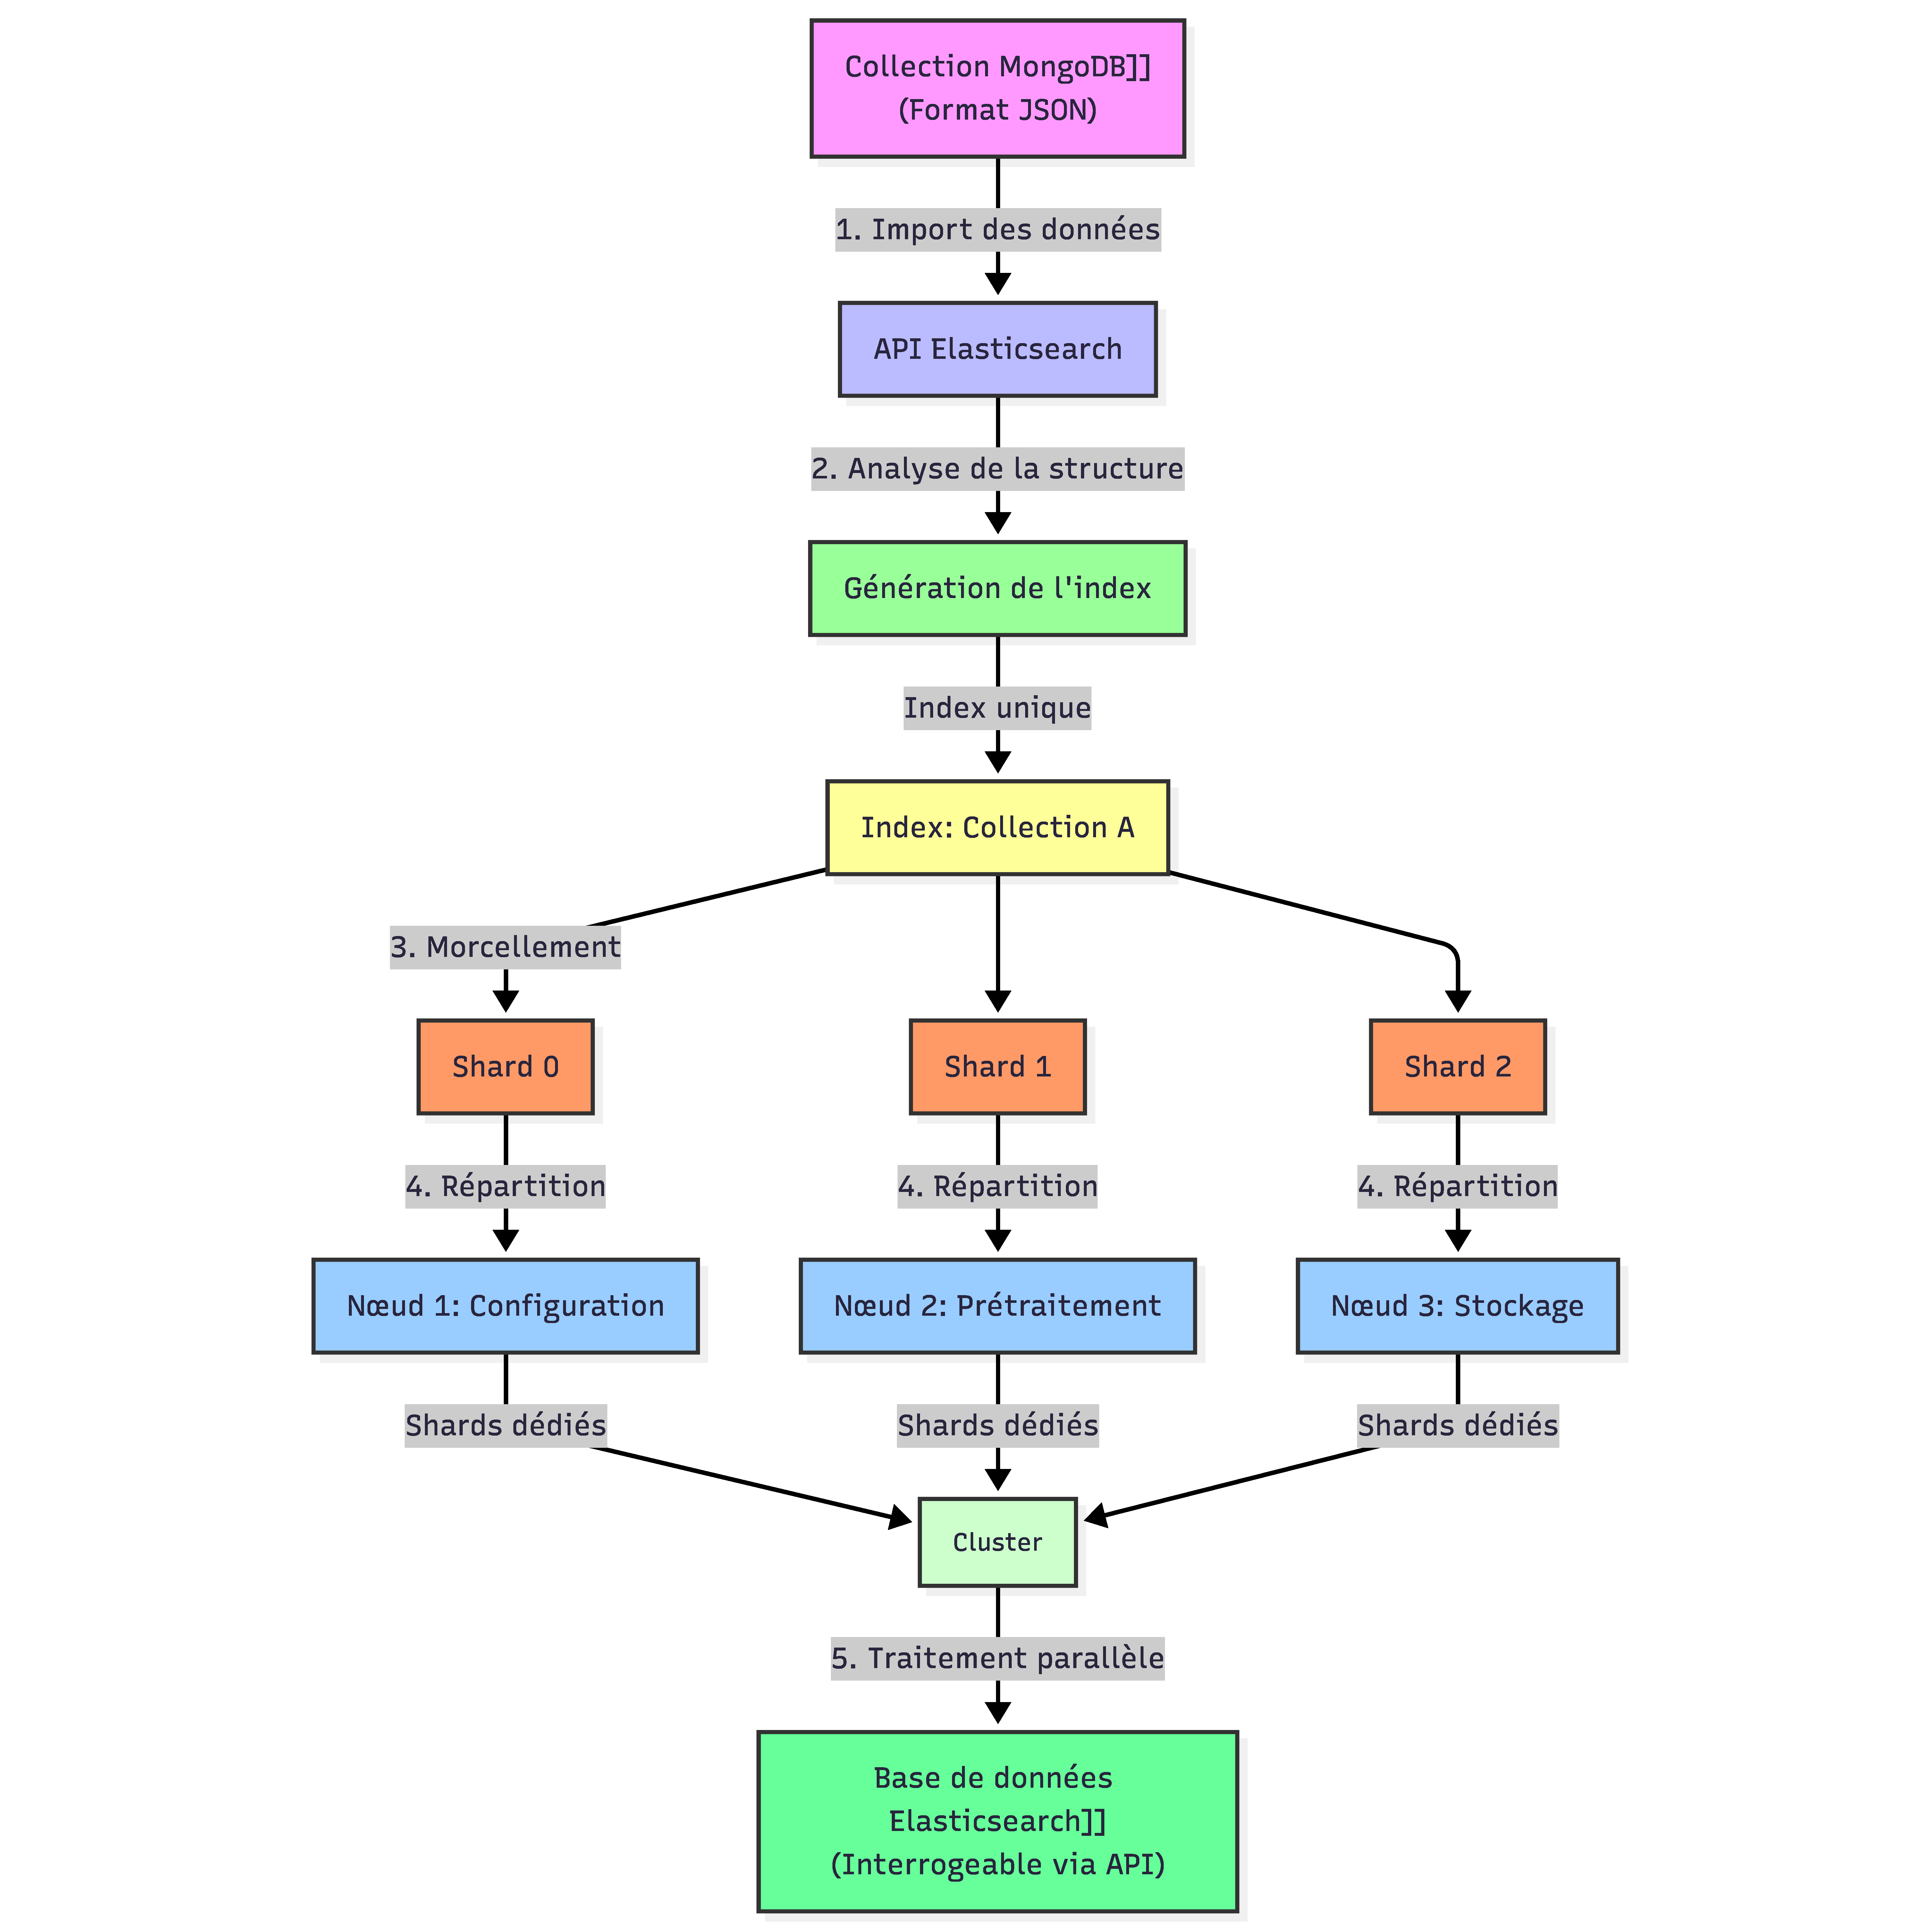
\includegraphics[width=0.8\textwidth]{./Schema/ElasticSearch.pdf}
	\caption{Schéma du fonctionnement d'Elasticsearch }
	\label{fig:elasticsearch_schema}
\end{figure}

\newpage

Ce système est donc lié à l'applicatif : il n'est pas un composant créé par l'application mais bien un élément externe relié à l'application. ElasticSearch propose ses propres modalités de recherche : recherche simple, recherche full-text\footnote{méthode de recherche qui explore des documents entiers à la recherche de chaîne de caractères demandées.}, recherche par mots-clés, recherche avancée ou bien par facettes, disons par catégorie et récurrence des données. Pour faciliter l'usage, l'application à créer une barre de recherche qui permet à l'utilisateur de créer ces requêtes de manière visuelle et interactive. C'est une interface \textit{no-code} qui permet d'envoyer les requêtes depuis l'application vers l'API ElasticSearch.\newline

\label{limites-SRI}Cependant, ces \gls{SRI} comme ElasticSearch rencontrent des limites dans l'exploitation des données des institutions patrimoniales. En effet,leurs structures ce sont largement complexifiées : d'abord par l'arrivée de nouvelles normes, modifiant des structures, et ensuite par le phénomène de densification des bases de données rendant leurs interrogation plus difficiles. Ces éléments n'ont fait que de mettre en évidences des limites déjà présentes, mais qui n'était pas forcément bloquantes. 

D'abord, ces systèmes ne prennent pas en compte la notion de contexte. La recherche s'effectue sur des critères de pertinences attribués par la correspondance de mots-clés. Ces mots clés sortent deux informations de leurs contextes : d'abord le mot qui peut avoir plusieurs significations en fonction du document et de la phrase, son contexte. Ainsi on risque d'avoir des résultats manquants de pertinence puisque la sémantique n'est pas intégrée. Ensuite, un document peut avoir un tout autre sens lorsqu'il est liés à un ensemble de documents. Or, l'analyse par mots-clés ne prend pas en compte cette notion. Ainsi, une recherche renverra vers une pièce d'archive d'un fonds mais pas vers les autres composants de ce même fonds. Seule la pièce pertinente sera renvoyée à l'utilisateur sans le fonds auquel il se rattache ce qui peut être bloquant pour un chercheur.

De plus, le système de correspondance par mots-clés des \gls{SRI} est fragile face aux variations d'indexation. Malgré les efforts de normalisation qui ont été menés, l'indexation humaine est par nature variable. Deux personnes vont décrire un même objet en utilisant des mots différents et le principe de correspondance par mots-clés est trop sensible à cette variabilités.\footcite[p.273]{koolenInformationRetrievalCultural2013} ElasticSearch, par exemple, s'appuie sur le modèle BM25 qui établi la pertinence en se basant sur la fréquence des termes. Il est donc en proie à deux limites : l'utilisations de même terme pour définir des réalités différentes d'une part, et leurs utilisations dans des contextes différents d'autres parts. Cela brouille les capacités d'analyses du logiciel ce qui impact la qualité et l'exhaustivité des résultats. En effet, un document présentant une fréquence de terme "pertinents" moins hautes qu'un autre ne signifie pas qu'il est moins pertinent. Le \gls{SRI} n'intègrent pas cette notion et propose donc des résultats parfois non pertinents. 
Cette limite peut être élargie au contenus même des documents historiques, de plus en plus renseignés dans les bases de données grâces aux technologies d'\gls{OCR} et d'\gls{HTR}. Le vocabulaire employé provoque une double difficulté : la correspondance sémantique et terminologique avec le langage actuel, et la variation de l'écriture d'un même mot à travers le temps. Les \gls{SRI} n'associent pas les termes historiques à des équivalents actuels ou à leurs évolutions orthographiques. Certaines recherches peuvent alors manquer d'outil précis.\footcite[]{ranjgarCulturalHeritageInformation2024} \label{Keyword}

Ensuite, ces systèmes sélectionnent les données pertinentes par proximité thématique. C'est à dire que des données se rattachant à des thèmes similaires sont retournées à l'utilisateur ensemble. Dans le domaine patrimoniale, des proximités thématique existent entre des typologies documentaires différentes, ce que les \gls{SRI} n'exploite pas puisqu'ils cloisonnent ces dernières.\footcite{koolenInformationRetrievalCultural2013}.\newline


Une autre difficulté est celle du cloisonnement terminologique des typologies patrimoniales. L'hétérogénéité des collections est prise en charge par la plus part des applications. SkinSoft le fait également à travers ces modules dédiés à chaque typologie\footnote{Voir page \ref{module}}. C'est ce qu'on appelle le traitement par silo : chaque typologie documentaire ayant son propre silo, schéma d'indexation et vocabulaire. Ainsi, les \gls{SRI} ont du mal à établir une porosité entre les silos ce qui ne reflète pas la réalité scientifique puisque des connexions sémantiques existent.\footcite[p.274]{koolenInformationRetrievalCultural2013} Pour le logiciel SkinSoft, cette limite est à nuancer : un outil de "recherche fédérée" permet de faire des correspondances entre ces silos. Ainsi, il est possible de rechercher à travers toutes les typologies documentaires via des correspondances de champs. Cependant, il y a des limites : seules certaines typologies documentaires sont interrogeable et uniquement sur un nombre restreint de champs. Car si des correspondances existent, elles ne sont pour autant pas évidente à traduire dans un \gls{SRI} qui est trop rigide.\newline
	
De plus, il y a un décalage entre croissant entre les pratiques des utilisateurs et les outils proposés par ces systèmes. Ce n'est que très récemment que des études ont été menées sur ce sujet\footcite{warwickIfYouBuild2007} et elles révèlent 3 problèmes fondamentaux : 
\begin{enumerate}
	\item D'abord, l'amélioration des navigateurs en lignes, tels Google, ont habitué l'utilisateur a fonctionner par échantillonage : la pertinence des résultats est analysée à partir de quelques pages seulement. Ainsi, quand les \gls{SRI} génèrent du bruit, il y a un désintérêt utilisateurs pour les résultats retournés.\footcite[p.9]{warwickIfYouBuild2007}
		
	\item \label{modalités-recherches} Ensuite, la complexité des interfaces de recherches. En effet, les utilisateurs n'ont pas l'habitude d'utiliser la recherche avancée, la recherche fédérée, les facettes, la recherche plein texte ciblée ou bien encore la recherche croisée propres aux \gls{SRI}. C'est une interface simple, qui renvoie des résultats pertinents et qui est donc bien plus attractive. Ainsi, aux yeux d'utilisateur ses outils perdent en intérêt et en praticité.\footcite[p.23-24]{warwickIfYouBuild2007}
		
	\item Enfin les \gls{SRI} ont leurs propres manière de structurer et indexer les données. Cela impacte directement la qualité des résultats retournés. Ces éléments sont cependant opaque, ce qui freine les chercheurs, notamment, à accorder une confiance complète aux résultats retournés. \label{opaque}
\end{enumerate} 
	
D'une manière plus générale, un utilisateur en face d'un outil opaque, proposant une interface complexe et des résultats bruités risque d'accorder moins de crédits au logiciel et s'en désintéresser.
	
Nous devons quand même nuancer ce propos. L'étude mentionnée traite des réactions et habitudes d'utilisateurs en tout genre face aux interfaces des sites d'institutions culturelles. Ce n'est pas une étude de comportement de professionnel face à des \terme{SGC}. 

Ainsi, l'impact des 3 points relevés n'est pas équivalents à ce qui est mentionné dans notre cas. Il est cependant une réalité que nos habitude d'utilisateur de moteur de recherche comme Google influence nos habitudes et attentes professionnelles. Au cours du stage, quelques retours utilisateurs m'ont permis d'associer les difficultés reportés dans l'article mentionné aux difficultées soulevées par des utilisateurs. C'est pour cette raison que figure ici ces limites, bien qu'ils soient nécessaire de les recontexualiser et de leurs accorder une moindre importance.\newline
	
Finalement, dans des collections toujours plus vastes et complexe, les \gls{SRI} ont de plus en plus de difficultés à satisfaire les exigences utilisateurs et scientifiques. La démocratisation des moteurs de recherches et des outils d'\gls{IA} changent drastiquement notre rapport à la recherche de données. Nos attentes et pratiques en mutation ont forcément un impact sur notre perception de ces outils, notre utilisations de ces derniers et donc leurs évolutions. 
	
C'est particulièrement visible dans l'outil SkinSoft reposant sur une base de donnée No-SQL de plusieurs dizaines de \gls{col} et aux données très variées. L'utilisation d'une indexation par mots-clés traditionnelles offre des performances limitées : on obtient facilement beaucoup de bruit à moins de savoircomment retrouver ce que l'on cherche. L'une des causes est la répétition des \gls{chps} dans l'application : un même champs peut apparaître plusieurs fois et contenir des données de nature différentes. De plus, SkinSoft propose son logiciel afin de gérer tous les types de collections : des plus petites et homogènes, aux plus vastes et hétérogènes. Plus la collections est vaste et hétérogène, plus le \gls{SRI} atteint ses limites et offre des performances moindre. 
	
L'\gls{SRI} est également mal adapté au principe de recherche fédérée. En effet, chaque typologie de collections est sujette à son propre module de gestion qui coexiste avec les autres. SkinSoft tire partie de cela par la recherche fédérée des modules permettant d'interroger plusieurs typologie de collections à l'aide des mêmes champs. Cependant, seulement quelques champs sont pris en comptes et le manque de compréhension contextuelle et syntaxique du \gls{SRI} est une grande limite.  
	
Ainsi, le logiciel SkinSoft cherche à améliorer son système de recherche par le \gls{NLP} afin de réduire le bruit généré, développer sa recherche fédérée, répondre à des requêtes plus exigeantes tout en offrant une plus grande simplicité d'usage. De plus, cela permettrais d'harmoniser les performances offertes par le moteur de recherche puisque cela permettrais de traiter plus facilement de plus grands jeux de données.\newline
	
Pour l'axe de l'amélioration de l'usage applicatif, nous nous retrouvons dans un domaine moins exploré. Deux éléments sont centraux : le premier est l'amélioration de l'usage utilisateur de l'application et de la compréhension qu'il en a. C'est à dire qu'on envisage le \gls{NLP}, notamment à travers un \gls{ac}, comme un moyen guider l'utilisateur au sein de l'application. Le second est de proposer un appui à la production de données patrimoniales propres et interopérables, toujours à travers un \gls{ac}. Il pourrait vérifier la saisie des métas données et les contradictions potentielles d'ordre sémantique. Ou encore les contradictions avec des normes descriptives appliquées aux domaines documentaires dans lequel on se trouve. Commençons par le premier point : 
	
L'agent conversationnel, comme ChatGPT, connaît une dyanmique de croissance technologique et de diffusion très importantes ces dernières années. L'outil se fait remarquer par sa capacité d'interraction avec un utilisateur par l'usage du \gls{NLP}. Cette caractéristique a tout de suite été vu comme l'opportunité de faire parler les collections et de faciliter les parcours utilisateurs sur les portails institutionnel. Plusieurs initiatives ont visées à concrétiser cette opportunité, comme celle des musées d'histoire naturelle Australien.\footcite{wangConversationalAIEnhancedExploration2026} 
	
Ces études ont amené à réfléchir sur les interfaces métier des \terme{SGC}. Il y a un véritable questionnement naissant sur l'impact des interfaces proposées dans les \guillemetleft logiciels métiers \guillemetright \footnote{Logiciel conçu pour répondre à des besoin professionnels.} \space sur la gestion des collections. 
	
Ces études abordent notamment la \guillemetleft surcharge cognitive \guillemetright \space, \label{cognitif} c'est à dire quand une interface propose trop d'informations et d'interractions différentes au point de perdre l'utilisateur.\footcite[p.1-4]{paasCognitiveLoadTheory2010}. Dans un \terme{SGC}, la principale source de surcharge cognitive est l'interactivité des éléments. En effet, un objet est reliés à énormément d'éléments individuel mais constamment en lien. Dès lors, la multiplicitées de ces connexions et leurs complexités peut surcharger l'utilisateur et conduire à faire des erreurs. Cela peut également créer une charge mentale encombrante pour l'utilisateur réduisant sa concentration.\footcite[p.2]{paasCognitiveLoadTheory2010} Cela relève de ce qu'on appel l'\gls{ux}, c'est à dire la manière de simplifier l'expérience utilisateur.
	
Le second point est celui de l'interface en elle même. L'interface reflète bien souvent la complexité logicielle et perd l'utilisateur dans son usage applicatif. La multiplications des points d'entrées par exemple dénue l'application de repère visuelle et exige une expérience de l'application. \footcite[p.153]{nielsenEnhancingExplanatoryPower1994} Plus important encore, l'interface est importante pour la gestion de l'information. Quand trop d'options ou d'actions sont proposées, l'informations essentielles à extraire ou intégrer échappe à l'utilisateur. Cela peut pousser un utilisateur à éviter ces endroits surchargés et donc ne pas utiliser certaines fonctionnalitées \footcite[p.153-154]{nielsenEnhancingExplanatoryPower1994}. Tout cela relève de ce qu'on appelle aujourd'hui l'\gls{ui}, où la manière de créer des interfaces logicielles pratiques et simples.
	
Le logiciel SkinSoft se heurte à certaines de ses complexités. Prenons les points d'accès : bien que groupés à un même endroit dans l'applicatif ils sont nombreux et produise un effet de masse. C'est le propre des logiciels de \terme{SGC} car la gestion d'un tel spectre de données mutliplient nécessairement les point d'accès. La simplifications de l'interface ne peut effacer cette première complexité car l'accès à chacun de ces points d'entrées est nécessaire. De plus, les interractions entre ces éléments sont nombreuses et demandent différentes fonctionnalités situées à différents endroits. C'est encore une fois le propre des \terme{SGC} : prenons l'objets, il reste au c\oe{ur} d'un bon nombre d'éléments ce qui fait de lui un n\oe{ud} central. Ainsi, il multiplie les points d'accès et les fonctionnalités associées : depuis un objet on peu créer un ensemble, un projet, une entrée, une sortie, un prêt, et bon nombre d'éléments.

Un autre problème rarement cités dans les études est la duplication de documentation externe. En effet, les fournisseurs logiciels produisent de la documentation métier destinées à guider l'utilisateur. Cependant, cette document n'est pas dans l'application : elle se trouve dans un dépôt externe. Ainsi, quand un utilisateur recontre une difficultés, il doit ressort de l'application afin de consulter un manuel, ou plusieurs. L'accessibilité à l'informations est un véritable problème : une réponse complexe à trouvée entraîne la perte d'intérêt.
	
Si des chercheurs proposent de décharger les interfaces afin de les rendres intuitives\footcite{whitelawGenerousInterfacesDigital2015}, l'ampleur de la tâche dans les \terme{SGC} est telle qu'on envisage de nouvelles solutions. Le logiciel SkinSoft le démontre bien : l'interface épurée, les efforts de regroupement d'éléments et de leurs répartitions ne suffisent pas à pallier la complexité native dû au \terme{SGC}. L'émergence des agents conversationnel ouvre une nouvelle possibilité : interagir avec l'application par de simple requête. De cette manière, il peut disposer d'un guide interactif qui a la capacité de s'appuyer sur cette documentation métier externe. Cet agent conversationnel peut d'ailleurs être le socle d'une technologie plus importante qu'est celle de l'agent IA, qui est capable lui d'interragir avec l'application.\newline
	
Pour le second point, très peu d'articles, pour ne pas dire presque aucun, ont été produit sur le sujet. Beaucoup énonce l'idée de faire de l'agent conversationnel un assitant de production, mais très peux y apporte une véritable dimension académique ou des propositions d'implémentation. C'est donc une partie bien plus théorique et expérimentale qui est abordée dans ce point. 
	
Des interfaces trop riches peuvent favoriser la saisie d'erreur dans les métas données, ce qui finit par constituer une bases de données instable. Mais ce n'est pas la seule explication : la redondance de la tâche ainsi que la difficulté à renseigner certains objets en sont des explications plus importantes encore. 
	
Ainsi, sur de large jeux de données, toujours en expansion, les moyens de contrôle actuels mis en place, comme des formulaires de saisies et des champs contrôlés, sont de plus en plus limitées.\footcite[p.2]{lewisImpactHumanDecisionMaking2025} En effet, plus la quantité de données à traiter est importante, plus la fiabilité humaine laisse place à des oublis, des erreurs de saisies et des incohérences de données. Si les erreurs sont très nombreuses et variées, les résulats lors du requêtage perdent en qualité\footcite[p.4]{lewisImpactHumanDecisionMaking2025}.
	
De plus, certaines collections spécifiques demandent des traitements particuliers. Prenons l'exemple des collections d'histoire naturelle, notamment des spécimens qui sont nombreux et centraux dans ces collections. Ils se rattachent à des classifications taxonomiques qui ne sont pas fixes : souvent hypothètiques, elles sont ensuite remaniées ou invalidées. Ces changements sont fréquents et concerne assez rapidement un grand nombre de specimens et donc de notice dans un \terme{SGC}. Il est donc souvent impossible d'assurer la mise à jour totale des espèces dans les grandes bases de données\footcite{hedrickDigitizationFutureNatural2020} Ainsi, un agent conversationnel capable de signaler à l'utilisateur la nécessité de mettre à jour certaines notices est particulièrement pertinent. Un agent IA capable de le faire seul, l'est d'autant plus.\newline
	
Le logiciel SkinSoft est un bon exemple des difficultées actuelles rencontrées par les \terme{SGC} et les limites des solutions déjà existantes. En effet, la simplification de l'interface et de l'expérience utilisateurs par l'application des principes d'\gls{ui} et d'\gls{ux} est limitées. La complexité native de ces systèmes ne peut être résolue entièrement de cette manière. La massification des données et l'hétérogénéité typologiques des collections constituent des défis demandant de nouveaux moyens de réponses. Ce manque de solutions est dû à un changement de problématique : la question n'est plus de faciliter, mais de créer de nouveaux outils pour combler l'écart entre la capacité de traitement humaine insuffisante face aux besoins du traitement des données massives et hétérogènes.
		
Ainsi, on comprends que l'intégration d'un agent conversationnel dans l'application a deux enjeux. Le premier enjeux est de simplifier la circulation et l'utilisation de l'application dans sa globalité. Cela est envisagé par la possibilité de converser avec un assistant spécialisé capable de guider en s'appuyant sur de la documentation métier contrôlée. Le second enjeux est donc de disposer d'un assistant capable de tracer l'activité faite, celle à faire et ainsi que la qualité de ce qui est déjà présent. De cette manière, il va pouvoir apporter une solution au problème principal que tout changement d'interface ne peut régler : la faillibilité humaine.
	
Le \gls{NLP} semble aujourd'hui apporté des éléments de réponses afin de combler cet écart. La capacité de cette technologie à interragir avec l'utilisateur et à comprendre les données à une échelle massive ouvre de nouvelles possibilités d'usages et d'interfaces qui permettrait de résoudres les problématiques relatives aux \terme{SGC}. Cependant, cette technologie recouvre un ensemble vaste d'outils et de réalités techniques\footnote{ Voir page \pageref{1.2.1}}, ce qui demande de les séparer en deux outils différents : la recherche augmentée, répondant aux problématique soulevées dans le premier point, et un \guillemet{chatbot}, répondant aux problématiques soulevées dans le second point.
	
	
	
	
	
	

	
\newpage
	
\section{Recherche augmentée et \gls{chatbot} : états de l'art.}

% !TeX root = ../document_maitre.tex

Les deux axes d'améliorations que nous venons de distinguer sont pensés en deux outils distincts. La \guillemet{recherche augmentée} : une recherche assistée par \gls{IA} pour interroger le \gls{SRI} en langage naturel. Et un \guillemet{\gls{chatbot}} pour disposer d'un guide et d'un appui au contrôle des données. Ces outils puisent dans la même source technologique mais sont des processus divergents à portées différentes. Ainsi, ils font l'objet d'interfaces différenciées.

Il existe aujourd'hui quelques projets et travaux académiques sur ces deux sujets. Ils ne sont pas nombreux et recouvrent des réalités techniques et professionnelles différentes aux nôtres. Il convient donc de présenter des états de l'art de chaque outil, à l'aide de ses connaissances, afin d'analyser les réalités techniques se cachant derrière ces fonctionnalités. Cela amène à des discussions sémantiques afin de lever des confusions terminologiques et techniques importantes, notamment autour du \gls{chatbot}. Nous en profiterons pour discerner les apports, limites et enjeux des technologies et processus cités.

\subsection{La \guillemet{recherche augmentée} : }

\subsubsection{La recherche intelligente}


L'origine de ce processus est la recherche intelligente, mis en place par les grands moteurs de recherche afin d'offrir des résultats pertinents sous forme de résumé.\footcite{flamentGoogleSGEAI2025}. Il vise à augmenter l'accessibilité utilisateur grâce au langage naturel et à offrir des résultats plus pertinents par l'interprétation de la phrase.\footcite{flamentGoogleSGEAI2025}. Fondement du reste de notre travail, il convient de l'explorer. Trois outils d'\gls{IA} le compose : le \gls{LLM}, le \gls{RAG} et les modèles de \gls{NLP}.\newline

Le \gls{LLM} constitue l'intermédiaire entre les données et l'utilisateur. Basé sur du \gls{DPL}, il mobilise les technologies du \gls{NLP} et les combine a une faculté de raisonnement. De cette manière, il est capable d'analyser et d'extraire la sémantique d'une phrase mais aussi de formuler ses propres phrases. Dans ce processus, il intervient au moment de la réponse afin de converser avec l'utilisateur. 
Pour cela il extrait des \glspl{tk}, c'est à dire des mots, de nos phrases qui sont analyser par différents processus de \gls{NLP}. Ils sont ensuite transformés en \gls{vcs}, une suite de chiffre unique, qui lui permettent de faire des liens sémantique et de \guillemet{comprendre}.

Le \gls{RAG} est le procédé au \coeur du processus car il permet de fiabiliser et contextualiser les résultats, réduisant les hallucinations des \glspl{LLM}. En effet, ce dernier peut parfois répondre à l'aide de ses propres \guillemet{connaissances} ce qui créer des éléments de réponses faussés. En connectant un \gls{LLM} à une ou plusieurs bases de données, on créer une source de connaissances vérifiée et validée par un opérateur humain sur laquelle il est contraint de s'appuyer. Pour répondre, le \gls{LLM} doit les analyser et les reformuler.\footnote{Pour plus d'informations sur le \gls{RAG} voir \pageref{rag}}

Les modèles de \gls{NLP} sont spécialisés sur des tâches précises telles que le \gls{POS} et le \gls{NER}. Ils sont appliqués successivement afin de mieux saisir le besoin profond exprimé dans une requête. Mais aussi de mieux comprendre les données stockées. Cela augmente la qualité de la \gls{Vecsion} et donc la pertinence des réponses. 

La combinaison de ces trois éléments permet de créer la recherche intelligente. On peut distinguer deux temps dans son fonctionnement. Le premier temps est une phase d'analyse, invisible par l'utilisateur. En voici un schéma :

\begin{figure}[H] \label{procrag}
\centering
\begin{tikzpicture}[
node distance=1.2cm,
% Définition directe des styles à l'intérieur de l'environnement tikzpicture
stepbox/.style={
rectangle,
draw=blue!80!black,
fill=blue!5,
thick,
rounded corners=4pt,
minimum width=9.5cm,
minimum height=1.2cm,
align=center,
font=\sffamily
},
arrow/.style={
->,
>=Stealth,
very thick,
draw=blue!80!black
}
]

% --- 1. LES SOURCES ---
\node (sources) [font=\sffamily\small, align=center, text=gray!80!black] 
{Sources de données : \textit{(PDF, Base de données, ...)}};

% --- 2. LES 4 ÉTAPES CLÉS ---
\node (e1) [stepbox, below=0.8cm of sources] {
\textbf{1. Connexion à la source de données}\\
\small Connecte l'outil aux données stockées.
};

\node (e2) [stepbox, below=of e1] {
\textbf{2. Analyse sémantique par modèle de \gls{NLP}}\\
\small \gls{POS}, \gls{NER}, \dots
};

\node (e3) [stepbox, below=of e2] {
\textbf{3. Indexation unifiée des données}\\
\small Réunis les données en un index permettant de classer les données.
};

\node (e4) [stepbox, fill=green!15, draw=green!60!black, below=of e3] {
\textbf{4. \Gls{Vecsion} des données indexées}\\
\gls{vcs} calculés à partir des données indexées.
};

% --- 3. FLÈCHES DE LIAISON ---
\draw [arrow] (sources) -- (e1);
\draw [arrow] (e1) -- (e2);
\draw [arrow] (e2) -- (e3);
\draw [arrow] (e3) -- (e4);

\end{tikzpicture}
\caption{Phase d'analyse de la recherche intelligente.}
\end{figure}

\newpage

Ce que l'on voit ici est principalement le mécanisme du \gls{RAG}. Une fois connectés à une source de données, il l'analyse grâce aux modèles de \gls{NLP}. Ainsi, on donne du sens sémantique à ces données dès lors considérées comme \guillemet{enrichies}. Elles sont ensuite réunies dans un index : comme un \gls{SRI}\footnote{Voir \fullref{Keyword}} le \gls{RAG} dispose de sa propre architecture de données. C'est sur cet index que la \gls{Vecsion} s'applique, créant des \gls{vcs} qui sont légers, plus faciles à interroger et plus fiables que l'index des données. Cela crée un double avantage par rapport à une recherche par mots-clés traditionnels. D'abord, une compréhension sémantique des données et ensuite une rapidité dans leur interrogation. En théorie, nos résultats gagnent en précision et rapidité.\newline

L'envoi d'une requête utilisateur formulée en langage naturel déclenche une nouvelle phase de traitement qui suit les étapes suivantes : 


\begin{figure}[H]
\centering
\begin{tikzpicture}[
node distance=1cm,
% Style des blocs standards
box/.style={
rectangle,
draw=blue!80!black,
fill=blue!5,
thick,
rounded corners=3pt,
minimum width=8.5cm,
minimum height=1.1cm,
align=center,
font=\sffamily\small
},
% Style des flèches
arrow/.style={
->,
>=Stealth,
very thick,
draw=blue!80!black
}
]

% --- LES ÉTAPES DU FLUX ACTIF ---

\node (e1) [box] {
\textbf{1. Réception de la requête}\\
\small Saisie de la requête en langage naturel
};

\node (e2) [box, below=of e1] {
\textbf{2. Analyse par NLP}\\
\small \gls{POS}, \gls{NER}, \dots
};

\node (e3) [box, below=of e2] {
\textbf{3. Vectorisation en direct}\\
\small Transformation de la demande en \gls{vcs}
};

\node (e4) [box, fill=purple!10, draw=purple!80!black, below=of e3] {
\textbf{4. Comparaison sémantique}\\
\small Mise en correspondance du \gls{vcs} de la requête aux \glspl{vcs} des données stockées.
};

\node (e5) [box, fill=green!15, draw=green!60!black, below=of e4] {
\textbf{5. Restitution des résultats}\\
\small Tri et affichage des réponses les plus pertinentes
};

% --- FLÈCHES DE LIAISON ---
\draw [arrow] (e1) -- (e2);
\draw [arrow] (e2) -- (e3);
\draw [arrow] (e3) -- (e4);
\draw [arrow] (e4) -- (e5);

\end{tikzpicture}
\caption{Phase dite \guillemet{active} de la recherche intelligente.}
\end{figure}

\vspace{0.1cm}

La phase \guillemet{active} de ce processus débute à l'envoi par l'utilisateur d'une requête en langage naturel. Ensuite on applique le même principe que précédemment : on comprend d'abord sémantiquement la requête à l'aide de modèles de \gls{NLP} avant d'opérer une \gls{Vecsion} des données composant la requête.

Ce sont les \glspl{vcs} qui sont ensuite comparés : des vecteurs proches signifient des correspondances sémantiques. Alors on vient chercher le sens profond de la donnée : l'idée qu'elle exprime. De cette manière on crée la capacité à saisir les idées représentées par les mots à une volonté. On ne s'arrête plus à la simple correspondance typographique.

Voici un schéma représentant le fonctionnement final d'un processus de recherche intelligente : 

\begin{figure}[H]
\centering
\begin{tikzpicture}[
node distance=0.9cm and 1.2cm,
% Définition des blocs et des flèches utilisées dans le schéma
box/.style={
rectangle,
draw=blue!80!black,
fill=blue!5,
thick,
rounded corners=3pt,
minimum width=6.5cm,
minimum height=1cm,
align=center,
font=\sffamily\small
},
passivebox/.style={
rectangle,
draw=orange!80!black,
fill=orange!5,
thick,
rounded corners=3pt,
minimum width=4.5cm,
minimum height=1cm,
align=center,
font=\sffamily\small
},
database/.style={
cylinder,
cylinder uses custom fill,
cylinder end fill=blue!20,
cylinder body fill=blue!10,
draw=blue!80!black,
thick,
aspect=0.25,
minimum width=3cm,
minimum height=1.2cm,
align=center,
font=\sffamily\small\bfseries
},
arrow/.style={
->,
>=Stealth,
very thick,
draw=blue!80!black
},
passivearrow/.style={
->,
>=Stealth,
very thick,
draw=orange!80!black,
dashed
}
]


% Phase d'analyse, située sur la gauche

\node (docs) [passivebox] {Données stockées\\(PDF, Bases de données, \dots)};
\node (doc_vec) [passivebox, below=of docs] {Extraction du sens par \gls{NLP} \\ et Vectorisation des données};
\node (index) [database, below=1.2cm of doc_vec] {Index de \glspl{vcs}\\des données stockées};

% Phase de requêtage, située sur la droite

\node (req) [box, right=2.5cm of docs] {1. Réception de la requête\\en langage naturel};
\node (nlp) [box, below=of req] {2. Analyse \gls{NLP} pour extraction du sens};
\node (vec) [box, below=of nlp] {3. \Gls{Vecsion} de la requête};
\node (comp) [box, fill=purple!10, draw=purple!80!black, below=of vec] {4. Comparaison des \glspl{vcs}\\ de la requête et de l'index};
\node (res) [box, fill=green!15, draw=green!60!black, below=of comp] {5. Retour des résultats pertinents \\ sur proximité des \glspl{vcs}};

% Création des flèches entre les blocs et phases

\draw [passivearrow] (docs) -- (doc_vec);
\draw [passivearrow] (doc_vec) -- (index);

\draw [arrow] (req) -- (nlp);
\draw [arrow] (nlp) -- (vec);
\draw [arrow] (vec) -- (comp);
\draw [arrow] (comp) -- (res);

\draw [arrow, draw=purple!80!black] (index) -- (comp) 
node[midway, above, font=\sffamily\tiny, text=purple!80!black] {Mise en correspondance};

% Définitions des cadres de regroupement
\node[draw=orange!80!black, dashed, thick, rounded corners, fit=(docs) (doc_vec) (index), 
inner sep=8pt, label=above:{\sffamily\bfseries\color{orange!80!black}I. Phase d'analyse}] {};

\node[draw=blue!80!black, thick, rounded corners, fit=(req) (nlp) (vec) (comp) (res), 
inner sep=8pt, label=above:{\sffamily\bfseries\color{blue!80!black}II. Phase de requêtage}] {};

\end{tikzpicture}
\caption{Fonctionnement global de la recherche intelligente.}
\end{figure}

Ce que nous avons décrit ici est un processus générique généralement modifié. Le \gls{chck} par exemple, permettant de fractionner des documents en plusieurs morceaux. Cela permet d'accélérer le traitement par la parallélisation de tâches\footnote{Désigne en informatique la capacité à traiter simultanément plusieurs tâches et données parfois dans des processus différents.} et de limiter la perte de précision par des analyses restreintes. Ce n'est qu'après qu'on peut extraire des \gls{tk}.\footcite{QuestceQueChunking} 

Ou encore le \gls{RR}. À l'issue du processus générique, les résultats les plus pertinents sont sélectionnés et classés selon un ordre d'importance. Le \gls{LLM} l'utilise afin d'organiser sa réponse. Cet outil consiste à évaluer la pertinence des résultats et les reclasser. Il effectue sa propre recherche dans les données stockées et les compare à la requête utilisateur, en fonction des divergences il refait un classement si besoin.\footcite{ultralyticsQuestCeQuun2026}\newline

Les limites restent importantes et mettent en doute la qualité scientifique des résultats. L'utilisation d'\gls{IAG} entraîne le risque d'hallucination et le \gls{RAG} limite mais n'annule pas ce risque. Notamment sur des requêtes basées sur des expressions imagées ou des termes spécifiques à des \guillemet{jargons} professionnels. Si le sens n'est pas saisi, il sera halluciné afin de créer une réponse tout de même.\footcite{cazzaroQueryingLLMsIf} 

De plus, ce processus ne peux procéder à des calculs d'agrégation de données. Ainsi, on en peut avoir recours à des calculs comme des moyennes, ce qui est essentiel dans certains domaines de recherches. \footcite{cazzaroQueryingLLMsIf} 

Ajoutons que la segmentation des documents par \gls{chck}, souvent utilisé, apporte des limites aux recherches complexes. Morceler les documents revient à multiplier les points d'informations et donc les calculs. Lorsqu'une requête amène à analyser un grand nombre de segments, le \gls{RAG} peut entrer dans un état de confusion et générer du bruit.\footcite{cazzaroQueryingLLMsIf} 

De plus, la recherche intelligente n'est pas transparente quant aux modalités de recherche. Le \gls{RAG} et le \gls{LLM} ne sont pas transparents dans leurs opérations et processus de réflexion. Ainsi, des doutes peuvent exister : a-t-il confondu des termes ? A-t-il halluciné ? A-t-il mal compris ? Toutes ces questions restent sans réponse et créent le même problème rencontré avec les \gls{SRI}\footnote{Voir page \pageref{opaque}}. 

Il y a aussi un enjeu de sécurité et de confidentialité des données. Il peut arriver que l'on souhaite ne distribuer que certaines informations à certaines personnes, ce qui est faisable grâce aux droits d'accès. Ces derniers sont difficiles à gérer sur des \gls{vcs}. Des systèmes le permettent, mais ils connaissent encore un certains nombre de faille trop importante posant le problème de la sécurité de l'information et de sa confidentialité. Deux principes clés dans nos institutions patrimoniales.

\subsubsection{Les processus \gls{2SQL} et \gls{2NSQL}}

L'objectif global est d'adapter le processus précédent aux technologies SQL et \gls{NSQL} dans des processus hybrides appelés :\gls{2SQL} ou \gls{2NSQL}. Ils présentent certains avantages :

Il n'y a pas d'hallucination : si la requête n'est pas comprise il n'y a simplement pas de réponse. Ils permettent des calculs mathématiques sur des données stockées en tant que chiffres. Et les requêtes complexes, multipliant les sources, ne sont pas sujettes à confusion grâce aux jointures pour le SQL et aux \gls{pipagreg} pour le \gls{NSQL}. Les requêtes sont compréhensibles par l'humain et re-jouable ce qui apporte une transparence au processus. Et pour finir, ils intègrent nativement des outils de contrôle des droits d'accès assurant la confidentialité des données. Le \gls{NLP} devient un outil de traduction vers le SQL ou \gls{NSQL} évitant la \gls{Vecsion} et l'interprétation de l'\gls{IA}. 

Cependant, il y a un manque considérable d'informations sur les projets menés à ce sujet dans notre domaine hors mis quelques approches spécifiques.\footnote{Nous ne développons pas ces approches plus poussées, mais les mentionnons par souci d'exhaustivité. Pour plus d'informations sur ces approches divergentes, consulter \cites{sergeevTalkingDataDesigning}{cazzaroQueryingLLMsIf}} Ainsi, nous allons expliquer de manière générale comment fonctionne un \textit{pipeline} \gls{2SQL} et \gls{2NSQL}. Commençons par mettre en exergue les trois difficultés majeures de cette adaptation : \newline 

D'abord, la compréhension des schémas SQL et du contexte métier. Les bases SQL ont une structure rigide créées sur les besoins de descriptions des institutions. Ces structures embarque des biais de recherches et d'exploitation définis selon une stratégie institutionnelle et les \guillemet{besoins métiers}\footnote{On parle de \guillemet{besoin métier} pour exprimer les besoins inhérent à un domaine professionnel et propre à ce domaine. Il correspond souvent à la réalité des pratiques employées par les professionnels.}. On attend de l'\gls{IA} qu'elle puisse comprendre un univers métier et institutionnel. On déplace ainsi le curseur de la compréhension des données stockées à celle de l'univers professionnel.\footcite{CommentObtenirCode}

Ensuite, la compréhension du besoin utilisateur. Si la recherche intelligente permet de rectifier les processus de réflexions de l'\gls{IA}, le \gls{2SQL} est moins souple sur le sujet. Pour changer cette réflexion cela demande de connaître la structuration de la base de données afin de guider le \gls{mod}. Cette compétence technique est cependant rare dans les institutions conservatrices ce qui amène le besoin de limiter les incompréhensions des requêtes et les interactions entre l'utilisateur et la base SQL.\footcite{CommentObtenirCode}

Enfin, la notion de \guillemet{[..] dialecte SQL [...]}\footcite{CommentObtenirCode}. Tout les systèmes de gestion des bases de données n'emploient pas exactement le même langage, et les \glspl{LLM} ont souvent du mal à s'adapter aux différences. Sur certains systèmes, la génération de requêtes complexes s'en trouve complexifiée et réactive le risque d'hallucination.\footcite{CommentObtenirCode}

Deux approches permettent de combler cet écart : les \textit{frameworks} spécialisés comme VANNA AI et les \gls{AGSQL} comme LangChain\footcite{TexttoSQLInterrogerVos2026}. La première approche consiste à créer un processus de \gls{RAG} avec le schéma SQL, des exemples de requêtes et de la documentation professionnelle. Ainsi, n'importe quel \gls{LLM} peut comprendre son environnement. Il atteint vite ses limites car chaque changement d'architecture de la base amène un changement de documentation et donc de résultats. La seconde approche est basée sur des \gls{LLM} spécialisé dans la compréhension et la génération de requête SQL y compris sur des bases complexes. Cet est outil est plus complexe à mettre en place et à maintenir. Qu'il soit basé sur un \gls{AGSQL} ou un \textit{framework}, un processus \gls{2SQL} ressemble à ceci :

\begin{figure}[H]
\centering
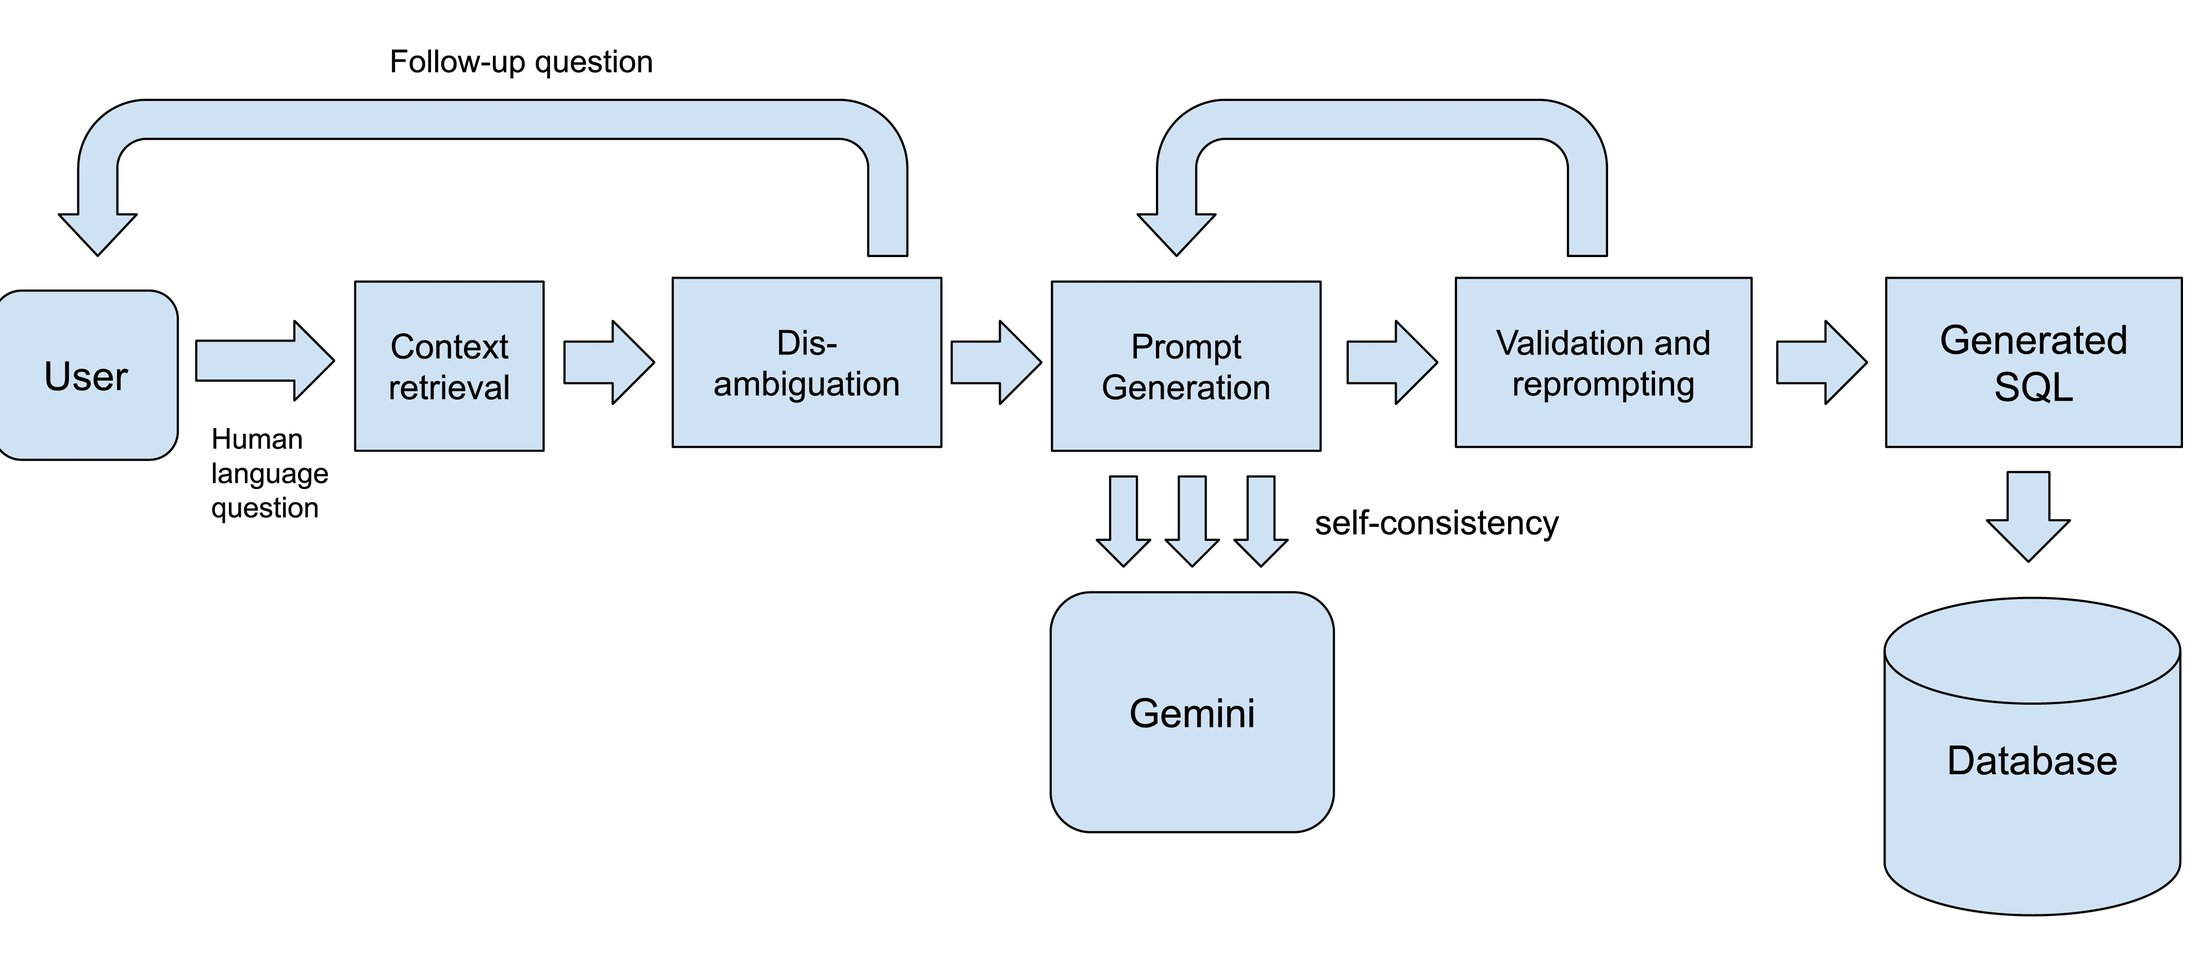
\includegraphics[width=0.8\textwidth]{./Schema/Text-to-SQL.png}
\caption{Schéma d'un pipeline \gls{2SQL}. Source : \cite{CommentObtenirCode}}
\label{fig:text-to-sql-schema}
\end{figure}

Nous en distinguons deux temps : le premier est consacré à la compréhension des besoins utilisateurs exprimés dans la requête initiale. Pour cela, on accorde la capacité au \gls{LLM} de relancer l'utilisateur à l'aide de question afin de clarifier le besoin. Il est essentiel pour cela que l'outil comprenne l’environnement métier dans lequel il s'inscrit. 

Le second temps est consacré à la génération de la requête SQL grâce au \gls{LLM}. D'abord il reformule la requête afin de la rendre plus compréhensible, augmentant la précision de la requête SQL générée. Cela donne naissance à un nouveau prompt généré par \gls{LLM} dans le seul but de générer du SQL. Ce prompt entre dans une boucle de traitement : il est examiné, puis soit refusé et reformulé soit validé ce qui entraîne la génération d'une requête SQL et son envoi à un \guillemet{parseur SQL}, un logiciel de vérification syntaxique des requêtes SQL. Cette requête est ensuite directement adressée à la base SQL en question. Dans le cas où l'institution possède plusieurs bases de données, le \gls{2SQL} peut s'y adapter. Soit par l'intégration d'un moteur de recherche fédéré, déclinant la requête selon l'architecture propre à chaque base, soit en laissant l'\gls{IA} déterminer quelle base de données est la plus pertinente afin de répondre à la requête.\newline

Le \gls{2SQL} se fait remarquer par sa capacité à s'adapter à toutes les bases de données existantes. De plus, ce processus assure des résultats fiables dès sa mise en place car il ne repose pas sur des \guillemet{connaissances} du \gls{LLM}, mais bien sur des métadonnées saisies par l'institution conservatrice assurant une plus grande véracité.

Il y a cependant quelques limites : d'abord, la dépendance à la \gls{DDL}, définissant le schéma de la base de données, et à la documentation métier. Si le schéma de la base, les pratiques et ou besoins métiers évoluent, une absence de mise à jour des documents amène l'échec du processus. Ensuite, son manque de scalabilité. Plus la base se complexifie, plus les requêtes se complexifier. En fonction du \gls{LLM} et des technologies choisies, la génération de requêtes complexes, comme des requêtes imbriquées, représente une difficulté plus ou moins importante. Cela peut alors conduire à des hallucinations de requête pouvant renvoyer les mauvaises données ou être invalide. Ce second cas finit par créer une boucle dans le processus : le \textit{parseur SQL} refuse de valider la requête et le \gls{LLM} continue cependant d'halluciner.\newline

\label{NoSQl} Un processus \gls{2NSQL} n'est pas très différent. Il repose sur l'exact même architecture \footnote{voir schéma du pipeline \gls{2SQL} page \pageref{fig:text-to-sql-schema}} et ne diverge que dans les implications techniques et les limites. 

Il y a trois variations techniques importantes. La première concerne la documentation à fournir. Une base \gls{NSQL} ne connaît pas de schéma fixe : chaque objet contenu, notamment dans les bases orientées documents, est défini selon son propre schéma. Sans structure globale fixée par une \gls{DDL}, le processus passe par une étape d'échantillonnage. Le \gls{LLM} parcours un nombre déterminé d'objets afin de cerner la variété des schémas. Sans la constance du schéma SQL on perd en fiabilité et en taux de réussite. À partir d'un échantillon, un \gls{LLM} ne peut pas se parer à toute éventualité augmentant le risque de se retrouver en situation d'échec ou d'hallucination.

La seconde variation intervient dans le rôle du \gls{LLM}. En \gls{NSQL}, on génère un \gls{pipagreg}. Cet outil fait passer chaque objet à travers des étapes de traitement successives, chaque résultat d'un traitement devient l'entrée du suivant. Ainsi on ne récupère pas les bonnes données brutes, mais les bons objets afin d'en extraire les bonnes données via les bons traitements. En somme, la sélection du document pertinent à partir d'une \guillemet{connaissance} par échantillonnage peut sembler \guillemet{hasardeuse}.

La dernière variation intervient sur la validation de la requête et son exécution. Dans un processus \gls{2NSQL}, il n'y a pas d'analyse syntaxique car le \gls{pipagreg} est plus souple, plus dense et donc plus complexe à examiner. La solution est l'exécution du \gls{pipagreg} dans un environnement de test. S'il semble fonctionner, alors il est exécuté sur les données. Cependant, ils sont complexes à générer car très verbeux et comprenant des syntaxes complexes auxquelles les \gls{LLM} sont encore peu habitués.

Ajoutons que les bases \gls{NSQL} sont de typologies variées : orientées documents, graphes ou bien colonne. Chaque typologie a sa propre manière de stocker les données et de les interroger. Ainsi, un processus \gls{2NSQL} créé pour une base de données \gls{NSQL} ne pourra pas s'appliquer à une base d'une autre typologie. Il y a donc une problématique d'\gls{intero} du processus le limitant à l'interrogation d'une seule base spécifique.\newline

Avant de conclure cette exploration des différents processus aujourd'hui existant pour améliorer la recherche sur des données, voici un tableau récapitulatif.

\begin{table}[H]
\centering
\small
\begin{tabularx}{\textwidth}{>{\bfseries}l X X X}
\toprule
Processus & Principe de fonctionnement & Apport & Limites \\
\midrule
Recherche intelligente & Indexation par \glspl{vcs} du langage naturel d'une base de données & Recherche sémantique et contextualisée via des \glspl{vcs} & Hallucinations, opacité, absence de calculs et risques de sécurité \\
\addlinespace[1cm]
Text-to-SQL & Traduction d'une requête en langage naturel en code SQL & Fiabilité des résultats, prises en compte des données structurées et gestion des droits & Dépendance à la \gls{DDL}, requêtes vites complexes et sclabilité difficile\\
\addlinespace[1cm]
Text-to-NoSQL & Traduction de requête en langage naturel en \gls{pipagreg} & Souplesse face aux structures des données, haute scalabilité & Fonctionne sur échantillonnage, absence de schéma fixe et manque d'interopérabilité\\
\bottomrule
\end{tabularx}
\caption{Comparaison des architectures des systèmes de recherche.}
\label{tab:pipelines_recherche}
\end{table}

Cette exploration de la recherche intelligente, du \gls{2SQL} et \gls{2NSQL} nous a amené à voir comment répondre aux enjeux actuels d'interrogation des données patrimoniales. Les processus \gls{2SQL} et \gls{2NSQL} permettent de faciliter l'interrogation des bases de données et d'optimiser les réponses obtenues. Résolvant ainsi les problèmes posés par les \gls{SRI} traditionnels ainsi que les enjeux d'accessibilité aux données.\newline

\label{hybride} Cependant, placer ces processus au sein de \glspl{sgc} pose des difficultés. Ces technologies sont dépendantes d'un socle de connaissance métier propre à l'institution. Le logiciel SkinSoft s'adressant à une pluralité d'institutions et de collections y rencontre une limite. Chaque institution a ses propres besoins, pratiques et enjeux métier auxquels la \guillemet{recherche augmentée} doit pouvoir y répondre.

De plus, les processus décrits ne prennent pas en compte l'usage d'un \gls{SRI} car ils visent à le remplacer. Cependant, la plupart de ces logiciels reposent sur cet outil. Ainsi, commence à être développée une approche hybride associant les \gls{SRI} aux approches méthodiques des processus \gls{2SQL} et \gls{2NSQL} que nous explorerons par la suite.\footnote{Voir \fullref{chap:Text-to-ES}}

Finalement, les expériences sont nombreuses mais les résultats concluants le sont moins. Ce principe de recherche intelligente appliquée au patrimoine ne cesse d'évoluer et de se diversifier, sans jamais vraiment réussir à satisfaire toutes les exigences. C'est donc un état de l'art très contrasté et l'expérience menée par SkinSoft est fondatrice pour les \glspl{sgc}

\subsection{Le \guillemet{chatbot}}

La majorité des recherches sur le \gls{NLP} dans le monde patrimonial ont porté sur les processus \gls{2SQL} et \gls{2NSQL}. Cependant, rendre la recherche de données plus facile et naturelle ne pas résout toutes les problématiques professionnelles.

En effet, une autre source de tensions provient des interfaces complexes et des nombreux parcours utilisateurs proposés. Notons que la production d'un professionnel dépend surtout de sa capacité à utiliser le logiciel et donc de sa clarté d'usage. Ainsi, la \guillemet{recherche augmentée} n'aborde pas cette problématique de front et n'y apporte pas de solutions.\footnote{Voir \fullref{cognitif}} 
Il faut chercher la solution dans un autre outil d'\gls{IA} : le \guillemet{chatbot}. Notons qu'aujourd'hui, le terme \gls{chatbot} porte un sens confus que nous devons clarifier.\newline

Malgré les première expérience concluantes en 1966 avec le programme ELIZA\footcite{adamopoulouChatbotsHistoryTechnology2020}, l'apparition du mot \gls{chatbot} date de 1994 avec le programme \textit{Julia}. Il interagit avec l'utilisateur en répondant avec des phrases grâce à un système de règles et de réponse prédéterminées. Il analyse la phrase, détermine à quel ensemble de règles elle se rattache et renvoie les réponses prédéterminées. C'est ce que l'on appelle l'\gls{IA} symbolique : il n'y a pas encore de \guillemet{réflexion}. Mais c'est cela que le mot \gls{chatbot} représente. 

Très vite, cette technologie est utilisée afin de diriger l'utilisateur vers les bons endroits dans le site. On utilise une interface simple : une fenêtre flottante avec un champs de saisie et un autre d'affichage.\newline

L'arrivée des \gls{IA} actuelles change le paysage du \gls{chatbot}. Sans règles, le programme est capable de réfléchir et de s'exprimer en autonomie ce que les \guillemet{\glspl{chatbot}} ne pouvaient pas faire. \footcite{adamopoulouChatbotsHistoryTechnology2020}
Leur capacité de génération et de compréhension ne faisant que grandir, les \guillemet{\gls{chatbot}} traditionnels ont peu à peu disparu. L'explosion public des \glspl{LLM} en 2020 a brouillé la barrière sémantique. Ils peuvent comprendre une requête, générer des réponses et mémoriser des conversations entières. Très différents d'un \gls{chatbot}, ils en adoptent pourtant la même forme dans ce que l'on appel les \glspl{ac}. Cela mélange les réalités technologiques car visuellement ce sont les mêmes outils. Ainsi, le terme \guillemet{\gls{chatbot}} finit par désigner les deux outils.

Très récemment, les \gls{LLM} ont commencé à se développer dans un autre sens : celui des \glspl{AGIA}. Si les \gls{ac} ont pour objectif de simuler une conversation avec un être humain, les \gls{AGIA} visent à accomplir des tâches complexes en autonomie. Un \gls{ac} converse uniquement, quand un \gls{AGIA} exécute des processus à l'aide d'outils. On constate, une nouvelle fois, que les \gls{AGIA} peuvent prendre la même forme que les \gls{ac} et \glspl{chatbot}.\newline

De nos jours, dans le langage courant, le terme de \guillemet{\gls{chatbot}} est profondément flous. Il désigne à la fois sa technologie historique, les \gls{ac} et les \gls{AGIA}.

Au sein de SkinSoft, la discussion autour de l'intégration d'un \gls{chatbot} dans le logiciel a fait ressortir cette évidente confusion. Lorsque l'on élargit le spectre à des projets et logiciels concurrents ayant implémenté un \guillemet{\gls{chatbot}} on se rend compte de la même imprécisions. Ainsi, dans ce présent mémoire lorsque nous parlons de \guillemet{\gls{chatbot}} nous désignons en réalité un \gls{ac}. Cela dans une volonté de s'inscrire dans une tendance terminologique actuelle et dominante. \newline

La question de l'intégration d'un \gls{chatbot} dans un \gls{sgc} est assez peu discutée. Cela peut s'expliquer par les risques d'hallucination dus à l'utilisation d'un \gls{LLM}. Notre attention doit se tourner alors vers les projets professionnels. 

Lorsque l'on regarde d'autres \gls{sgc} comme Axiell\footnote{Pour consulter leurs innovations, voir : \url{https://www.axiell.com/fr/solutions/product/ai-for-museums-and-archives/}}, ou Terentia \footnote{Pour consulter leurs innovations, voir : \url{https://terentia.io/collections-management}} on remarque les éléments suivants. D'abord, les termes de \gls{chatbot}, de \gls{ac} ou de \gls{AGIA} ne sont pas employés. Il est fait mention \guillemet{d'outils d'\gls{IA}}, sans plus de précision. Les outils cités semblent peu orientés vers l'accessibilité applicative et les questions d'usages. Que ce soit chez Axiell ou Terentia, les \guillemet{outils d'\gls{IA}} ont pour buts principaux de produire de la métadonnée et de faciliter des liens avec des thésaurus externes. En somme ce sont de nouveaux outils pensés pour compléter les fonctionnalité déjà présentes.

En combinant le \gls{RAG} sur de la documentation métiers et les capacité d'un \gls{chatbot}, nous pouvons obtenir un véritable assistant à l'utilisation de l'application. Ce système a déjà été appliqué à l'exploration de corpus documentaires afin d'accompagner les chercheurs dans leurs explorations. \footcite{tuzaInterrogerMemoireDentreprise2025} Cela permet des approches approfondies de corpus importants plus rapidement grâce aux capacités de conversation et de réflexion des \glspl{chatbot} limités par un \gls{RAG} aux seuls corpus.\newline

La problématique réside dans le choix de la documentation. Le \gls{RAG} demande de la documentation limitée et uniforme ce qui n'est pas le cas dans notre univers métiers. Les normes, standards, modèles conceptuels et politiques institutionnelles prennent des formes très différentes. Il se peut d'ailleurs que fournir une telle diversité de documentations technique au \gls{RAG} l'incite à commettre des erreurs. Il peut appliquer des concepts d'autres typologies patrimoniale et une typologie tierce.\newline

Il est difficile de faire un état de l'art de cette emploi, encore peu répandue, de cette technologie. Cependant, notre rapide examen permet de conclure que cette perspective est encore expérimentale et semble rencontrer bien des soucis de définitions.

Cependant, les capacités conversationnelles du \gls{chatbot} et d'intégration dans des processus plus larges permettent d'envisager cette technologie pour facilité l'utilisation des \glspl{sgc}.

\newpage

\section[Enjeux utilisateurs]{Enjeux utilisateurs : comment implémenter ces fonctionnalités en respectant l’utilisateur dans son usage de l’application et son rapport avec l’intelligence artificielle ? }	

% !TeX root = ../document_maitre.tex

\label{uxui}


Avant toute choses, notons qu'il s'agit ici d'une partie réflexive qui n'a pas pour objectif d'aboutir à des solutions concrètes. L'ambition est de présenter un état des lieux et des pistes de réflexions pouvant être l'objet de logiques d'implémentations et d'usage de ces outils.\newline

Lors de notre exploration du \gls{chatbot}, deux notions fondamentales ont été évoquées : l'\gls{ux} et l'\gls{ui}. Ils visent à placer l'utilisateur au c\oe{ur} des conceptions logicielles car l'usage utilisateur offerte défini l'attractivité et la qualité logicielle. Ils visent alors à garantir une utilisation optimale, fluide et intuitive d'un logiciel par le respect d'un certains nombres de principes, de normes et de méthodes. On y distingue l'expérience, gérée par l'\gls{ux}, et l'interface, gérée par l'\gls{ui}.

Arriver à garantir ces aspects permet de renforcer l'adoption du logiciel au près du public cible. Au c\oe{ur} de ces aspects se trouve l'expérience utilisateur, c'est à dire l'ensemble de ressenti, sensations et \guillemet{émotions} qu'une utilisation de l'application produit ou doit produire. L'\gls{ux} vise à garantir une expérience globale positive et qualitative lors de l'interaction entre l'utilisateur et l'application.\footcite{groupeLUXDesignDefinition2022} Un certains nombre de principes et de règles\footnote{Notamment \cite{ISO92411122025}} constituant ce domaine sont déterminées dans cet objectif. L'\gls{ux} régit un aspect pratique créé au moment de l'élaboration et du codage du logiciel, mobilisant ainsi un certains nombre de méthodes pour concevoir une expérience idéale dans une application orientée utilisateur.\footcite{lallemandMethodesDesignUX2018}

L'expérience utilisateur est transmise au travers d'un intermédiaire spécifique qu'est l'interface. Pour l'utilisateur l'interface fait partie intégrante de l'expérience globale, du côté des développeurs l'interface se différencie de l'expérience car n'étant qu'un outil de diffusion et d'interactivité. Ainsi, la création d'interface qualitative permettant une interaction \guillemet{positive} entre l'utilisateur le logiciel est régi par son domaine propre : l'\gls{ui}. Les fondements de ce dernier sont profonds. Dès 1990, le psychologue Don Norman démontre la responsabilité des \textit{design} dans les erreurs humaines dans un contexte industriel : \textit{\guillemet{Most industrial accidents are caused by human error: estimates range between 75 and 95 percent. How is it that so many people are so incompetent? Answer: They aren’t. It’s a design problem.}}\footcite{normanDesignEverydayThings} C'est le fondement de ce domaine : une interface mal conçue entraîne nécessairement une erreur. L'\gls{ui} a pour objectif de traduire l'\gls{ux} via des repères visuels et des parcours graphiques permettant d'activer des fonctionnalités. À l'instar de la notion précédente, l'\gls{ui} s'appuie sur des principes graphiques pour créer des interfaces intuitives au service de l'utilisateur. \newline

Soulignons que ces domaines ne sont pas rigide et ne posent pas de contraintes ni d'obligations. Ils ne font que proposer des méthodologies et outils obéissant à des principes et règles pensées pour atteindre des objectifs. Chaque développement logiciel n'a pas d'obligation à les utiliser ou à en respecter les principes. Ils peuvent adapter ces éléments où bien créer leurs propres principes, règles et méthodologies. 

Prenons l'exemple de la norme ISO 9241-112 abordant la question de l'expérience et interface des systèmes informatiques. Elle ne fixe pas de cadre rigide et obligatoire, elle \guillemet{[...] énonce des principes de conception ergonomique pour des systèmes interactifs dont la présentation d'information de l’interface utilisateur est contrôlée par logiciel}\footcite{ISO92411122025}. Son objectif est de proposer des principes clés pour conceptualiser une structure logicielle optimisée pour la compréhension des informations par l'utilisateurs. Il subsiste une certaine liberté et un flou conceptuel qui rendent l'application de ces concepts parfois délicate.

\subsection{\gls{ux} et \gls{ui} dans les \glspl{sgc} :}

Nous l'avons déjà exploré, les \glspl{sgc} sont des applications aux architectures denses et complexe ce qui impact nécessairement l'expérience et l'interface. Ils sont basés sur l'intégration d'une multiplicité d'informations avec une haute interactivité entre elles réparties dans de multiples fonctionnalités. Une notice d'objet disposera de ces propres fonctionnalités et interfaces, de même pour une notice de prêt. Ainsi, les interfaces sont multiples car elles correspondent à des expériences multiples adaptées à des modalités de gestion spécifiques. Cette multiplicité de parcours entraîne des complexités structurelles dans l'organisation de l'application et des données contenues et diffusées.

Dans ce contexte, l'\gls{ux} et l'\gls{ui} sont fondamentales pour simplifier l'apparence et l'usage d'outils destinés à manipuler de très grands volumes de données et à appuyer des décisions stratégiques. Il n'existe aucun principes, règles ou méthodologies spécifiques à l'application de ces domaines aux \glspl{sgc}. Cela s'explique par l'existence de questionnement et de contradiction, entre les principes généraux de ces domaines et les besoins auxquels répondre. La conception de ces domaines vise à simplifier l'usage applicatif et l'affichage par une logique d'épuration pour plus d'efficacité. Cependant, les besoins patrimoniaux au c\oe{ur} de la raison d'être de ces logiciel est l'exhaustivité des données ou plutôt la possibilité d'interagir avec des données dans toutes leurs complexités. Cette logique amène à dupliquer les expériences utilisateurs et à charger les interfaces avec deux informations : des fonctionnalités, représentées par des boutons dit d'actions, et les données stockées. 

\textbf{inclure une photo}\newline 

Aujourd'hui, des discussions académiques et professionnelles amènent à repenser ces notions appliquées aux \gls{sgc}. Deux idées principales en émergent : l'application du concept de simplicité sans tendre vers l'épuration, limitant l'exhaustivité naturelles de ces collections, et la recherche de nouvelles solutions d'interactions et graphiques. L'idée étant de simplifier l'exhaustivité, et non de la limiter et de la biaiser ce qui est aujourd'hui le cas lorsque l'on parle de rationalisation des interfaces et expériences utilisateurs. 

De plus, on ne s'adresse pas à des utilisateurs grands publics mais à des professionnels aux objectif précis et aux contraintes professionnelles devant être prise en compte. Ces objectifs et contraintes professionnelles varient en fonction de la typologie de collections traitées et de l'aspect de la collection qui est traité. On peut imaginer qu'une collection d'histoire naturelle ne demandera pas les mêmes expériences et interface que pour une bibliothèques. \newline

Aujourd'hui, des tentatives de compromis entre simplicité, exhaustivité et particularité de chaque collections tendant à apparaître dans une logique de communication vers un large public.\footcite{whitelawGenerousInterfacesDigital2015} On peut tout à fait s'attendre à voir émerger le souhait d'une cohérence de traitement, poussant les \gls{sgc} dans cette direction. A savoir : l'utilisation de moyens graphiques \textit{(comme des graphes)} pour représenter l'envergure de la collection et s'adapter à des usages et objectifs précis.\footcite{whitelawGenerousInterfacesDigital2015}

Aujourd'hui, les ambitions d'\gls{ux} et d'\gls{ui} appliquées à des \gls{sgc} semblent suivre la voix tracée par deux éléments. D'abord, la théorie de la surcharge cognitive\footcite{paasCognitiveLoadTheory2010} qui démontre qu'une surcharge informationnelle impact directement la productivité utilisateurs en réduisant les capacité d'attentions et de concentration de l'utilisateur. Transposé à un environnement logiciel, un surplus d'outils et de données risque d'entraîner une saturation chez l'utilisateur conduisant alors a un rejet du système. Ce phénomène est au cœur du (\textit{Technology Acceptance Model})\footcite{baddaTechnologyAcceptanceModel2025}, rappelant que l'utilité perçue et la facilité d'utilisation conditionnent directement l'adoption d'un outil. Modèle vers lequel les logiciels présentant de tels densités d'informations tendent aujourd'hui à appliquer. 


\subsection{Les outils d'\gls{IA} :}

L'inclusion de l'\gls{IA} dans toutes sortes de logiciel bouscule la réalité de l'\gls{ux} et de l'\gls{ui}. En effet, il est tentant de considérer le développement de fonctionnalités basées sur l'\gls{IA} comme identique aux autres développement mais ce n'est pas tout à fait la réalité. \newline

Les outils d'\gls{IA} sont souvent développés par des entreprises externes sans lien avec le système souhaitant l'inclure. Ils sont donc pensés indépendamment de systèmes tierces, avec leurs propres interfaces et expériences. Ceci pose un premier défis qu'est celui de l'inclusion de l'outil à inclure dans le système. L'outil possède ses propres besoins et propositions d'expérience et d'interface de même que le système hôte ce qui peux créer un important décalage entre les éléments et poussant à adapter son \gls{ux} et \gls{ui} d'origine afin de créer un dialogue entre les deux éléments. 

Ajoutons également que ces outils entendent parfois \guillemet{révolutionner} certaines pratiques et procédure communes. Ceci pose la question des habitudes utilisateurs et de leurs changements, ce qui peux impacter la qualité d'expérience globale. En effet, trop changer en profondeur une fonctionnalité habituelle peu déstabiliser un utilisateur, parfois définitivement. Par exemple, l'apparition d'un \gls{chatbot} peut être destabilisant : on est dès lors capable de converser à travers une fenêtre dédiée et de l'utiliser pour effectuer des tâches différemment, voir parfois les automatiser.

Pour finir, l'utilisation d'\gls{IA} pose aussi la question de la transparence. Nous l'avons vu, ces outils agissent sur des données parfois personnelles et/ou sensibles et des questions légales et éthiques impose une obligation de transparence. Cela dans le but que l'utilisateur puisse savoir les données utilisées, dans quels buts ses données sont utilisées notamment. Cela demande donc de créer une expérience rassurante et transparente, amenant à modifier les interfaces pour permettre la diffusion de ces nouvelles informations.\newline

Ces quelques points nous permettent de comprendre que l'intégration d'\gls{IA} dans des logiciels demande plus que la création d'une fonctionnalité technique. Il faut aussi, et surtout, réussir à intégrer de nouvelles expériences et interfaces rassurantes dans des cadres préexistants sans perturber l'utilisateur. C'est une tâche difficile dont dépend l'adoption de ces outils par les utilisateurs. 

\subsection{\gls{IA} et \gls{sgc} : des attentes \gls{ux} et \gls{ui} particulières}

L'inclusion d'outils basés sur l'\gls{IA} dans des \gls{sgc} pose des problématiques particulières. Les utilisateurs sont des professionnels souvent alerte sur l'utilisation des données par ce type d'outils, sensibles à la conservation de leurs données et engagés dans des démarches de rigueur scientifique. Ainsi, trois aspects semblent être au c\oe{ur} de tensions : \newline

D'abord la confiance envers l'outils. Malgré des efforts de contrôles, l'hallucination reste fréquentes et gênantes. La gestion des données patrimoniales est gouvernée par un besoin d'exactitude scientifique autant dans sa production que dans sa recherche. L'hallucination peu compromettre cette rigueur et entraîner une méfiance, un désintérêt légitime voire un rejet de l'outil. L'\gls{ux} doit pouvoir prendre en compte ses éléments en proposant des solutions comme des processus dit \textit{humain in the loop} et de gestion des erreurs, plaçant ainsi l'utilisateur comme contrôleur de la qualité des données et donc en position de contrôle. 

Le second élément est celui de l'interactions de ces outils avec l'environnement logiciel préexistant. Par exemple, la recherche augmentée comme le \gls{chatbot} génèrent de la donnée en masse pouvant amener à créer une surcharge informationnelles. La problématique se situe dans l'insertion de ces outils dans des environnements métiers déjà maîtrisé par l'utilisateur. Il faut s'assurer que ces outils amènent une plus values, qu'ils permettent une simplification des parcours d'usages sans créer des incohérences de parcours.

Le dernier élément est celui de la perception. Notre examen de la recherche intelligente démontre que le public auxquels on s'adresse aujourd'hui est méfiant envers les \glspl{IA}. Ceci peut expliquer partiellement le manque de travaux sur l'utilisation de \gls{chatbot} dans la production et la gestion de données patrimoniales. Faire de ces outils de véritables assistants à la productivité plutôt que des contraintes visuelles et technique constitue un enjeu majeur.

\subsection{Conclusion}

L'intégration du \gls{NLP} en deux outils différents, la recherche augmentée et le \gls{chatbot}, soulève des problématiques d'\gls{ux} et d'\gls{ui} inédites. Il ne s'agit pas d'ajouter des fonctionnalités supplémentaires ou de modifier légèrement une expérience utilisateur et l'interface. Il s'agit de changer drastiquement des éléments préexistant par un changement de rapport et de dialogue entre l'utilisateur et son système professionnel dans un domaine exigeant et attentif aux questions de sécurités et de qualités. 

Ces nouveaux outils doivent donc amener la conception de nouvelles expériences et interfaces respectant les exigences professionnelles fortes et réduisant la surcharge visuelle et cognitive. Ou du moins, ne pas l'alourdir. 

Il faut penser à l'adoption de ces technologies plus qu'aux simples performances technologiques. Cette adoption passe par la nécessité d'un dialogue transparent entre l'outil et l'utilisateur, placé au c\oe{ur} du processus. Ce qui déplace les enjeux de l'\gls{ux} et l'\gls{ui} des questions visuelles et de confort vers des questions de confiances et d'accessibilités.

\chapter[Traitement et indexation de l'\gls{imgani}]{Faciliter l’indexation par sa semi-automatisation : le cas de l’image animée}

\section[Dans le logiciel Skinsoft]{La gestion de l’image animée dans le logiciel SkinSoft}

% !TeX root = ../document_maitre.tex

\label{imageAnimee}

Dans cette partie, l'indexation semi-automatisée est pensée dans son application à un objet patrimonial particulier : l'\gls{imgani}. Les spécificités de cet objet et sa complexité d'indexation, même humaine, le placent au \coeur des volontés d'automatisation de son indexation et en démontrent les limites.

\subsection{Définition de l'indexation et de l'\gls{imgani} }

L'indexation est une opération d'analyse et d'extraction d'informations contenues par les objets patrimoniaux afin de produire des métadonnées descriptives attribuant des caractéristiques uniques à chaque objet. Pour cela, l'indexation s’appuie sur différents outils comme des \gls{thesaurus} afin d'en faciliter l'exécution et de créer une homogénéité.\footcite[p.2]{directiondesarchivesdefranceNoteDinformationDITN2007} Sa \guillemet{semi-automatisation} est l'idée de pouvoir se reposer partiellement sur des outils \gls{IA} capable de proposer des métadonnées dans les bons champs, respectant les normes et standards. L'opérateur humain n'ayant plus qu'à valider ou modifier ce dernières.

Pour penser de tels processus appliqués à l'\gls{imgani}, il convient d'en comprendre la nature et complexité. La \gls{FIAF} la définit comme un objet regroupant des images enregistrées successivement dont la diffusion donne une impression de mouvement.\footcite[p.5]{fairbairnManuelCatalogageImages} Cela peut être un \gls{rush}, c'est-à-dire l'enregistrement brute, ou bien une version retravaillée en \guillemet{post-production}. Elle peut intégrer des bandes sonores enregistrés au moment de la capture des images ou rajoutées en \guillemet{post-production}. Ainsi, un film, une vidéo, un extrait, une bande-annonce, une publicité sont des \glspl{imgani}.

Elle se caractérise également par sa diversité matérielle. L'\gls{imgani} a d'abord été enregistré sur des bandes au nitrate d'argent photosensible. Puis sur des bandes vidéos magnétiques permettant l'enregistrement sonore en simultané. Puis sur des supports optiques gravés, comme les DVD. Et enfin les supports numériques, tels des clés USB ou des \textit{clouds}, les stockant dans des formats digitaux comme le MP4 le MKV. Ils servent à l'enregistrement original et/ou à la diffusion. Pour le format numérique, on distingue les formats numériques de production des formats numériques de diffusion. Les formats varient en fonction du matériel utilisé pour enregistré et celui utilisé par diffusé. Pour des raisons de conservation on rencontre un principe similaire sur l'\gls{imgani} physique, ce qui fait qu'une même \oe{uvre} existe dans différentes matérialités simultanément ou successivement.\newline %pour l'absence d'un \gls{oe}. Je ne fais pas référence au niveau WEMI donc inaproprié.

Il y a également une notion d'état amené par la \guillemet{post-production}. Prenons un film récent comme \textit{Avatar (2009)} du réalisateur James Cameron. Le film diffusé au public est uniquement fait d'images de synthèse et d'effets spéciaux numériques. Cependant, tout cela a été produit à partir de \glspl{rush} sur lesquels figurent des acteurs, d'autres décors et matériels. Il existe donc deux états du film : la version \guillemet{brute}, composé de \glspl{rush}, et la version diffusée. Ces transformations extrêmes restent rares, cependant la \guillemet{post-production} a tendance à prendre une place grandissante.\newline

L'\gls{imgani} nécessite un matériel de diffusion. En effet, sa projection est un aspect fondamental car c'est ce qui fait apparaître la notion de mouvement. Cela implique la conservation des équipements de diffusion propres à chaque matérialité de l'\gls{imgani}.\footcite{edmondsonPHILOSOPHYPRINCIPLES} Cela demande donc d'entretenir ce matériel précieux, certains équipements n'étant plus fabriqués. Il y a donc une double obsolescence : celle des supports de diffusion et celle de l'objet patrimonial. Ainsi, une \gls{imgani} produite au début du XX\textsuperscript{ème} siècle sur une bande en nitrate d'argent et doublement en danger. D'abord par sa conversation, son composé chimique étant instable et pouvant prendre feu si mal conservé. Ensuite pour sa diffusion, le projecteur n'étant plus fabriqué et les compétences pour l'entretenir se raréfie.\footcite[p.39 et 54]{edmondsonPHILOSOPHYPRINCIPLES}

Il y a également une grande diversité conceptuelle. Nous ne parlons pas de film, de vidéos ou encore de documentaire car ils représentent des réalités différentes leur réalisation, utilisation, objectif, diffusion et conservation. L'\gls{imgani} concerne aussi bien un film amateur que professionnel, et toutes la typologie que cela recouvre, mais aussi les séries, publicités, etc.\footcite[p.5]{fairbairnManuelCatalogageImages}. Chaque typologie possède ses caractéristiques uniques et donc sa propre indexation.\footcite[p.18 et 34]{edmondsonPHILOSOPHYPRINCIPLES}\newline

C'est un objet patrimonial unique, faisant face à ses propres défis non partagés avec les autres objets patrimoniaux. Dès lors, au sein de collections hétérogènes l'indexation de l'\gls{imgani} se doit d'être particulière afin de prendre en compte toutes les complexités brièvement explorées.

\subsection{Le \gls{FRBR} et le \gls{WEMI}}

\label{FRBR-WEMI}

Les prémices de cette gestion particulière apparaissent en 1998. Jusqu'alors, la norme internationale qu'est l'ISBD structurait les données bibliographiques autour du seul objet physique. Cela ne permettait pas de créer du lien au sein des collections internes et externes et l'apparition de déclinaisons, comme l'ISBD(A) pour les livres anciens, a finalement fragilisé l'homogénéité des données. Devant l'évolution des besoins utilisateurs, visant à simplifier les requêtes, l'ISBD s'est révélé peu adapté. Une \oe{uvre} ne pouvant être présentée avec ses déclinaisons successives, ni ses liens avec d'autres \oe{uvres}, la démarche exploratoire de l'utilisateur s'est retrouvé trop limité et frustrante. 

Ainsi, l'\gls{IFLA} souhaite réorganiser la gestion de cet objet patrimonial en déplaçant le point d'intérêt de l'exemplaire vers un ensemble conceptuel plus vaste et structuré. C'est le \coeur du modèle \gls{FRBR} qu'elle publie afin de repenser tout ce système de description et de gestion des données bibliographiques.\footcite{universalbibliographiccontrolandinternationalmarcprogrammeFunctionalRequirementsBibliographic1998}\newline  

Il répartit les données bibliographiques en 3 groupes d'informations.\footcite[P.12 à 16]{universalbibliographiccontrolandinternationalmarcprogrammeFunctionalRequirementsBibliographic1998} D'abord le groupe des informations sur le contenu intellectuel et artistique de l'\oe{uvre} indexée. Elles sont réparties sur 4 entités hiérarchisées, représentant chacune un niveau d'indexation de l'\gls{oe}. Ce sont les niveaux \gls{WEMI} pour : \gls{oe}, ou \gls{oe}, \gls{exp}, \gls{man} et \gls{it}. 

L'\gls{oe} est le niveau hiérarchique le plus haut, représentant l'idée intellectuelle ou artistique sans matérialité définie. C'est l'élément central auquel les niveaux \gls{exp}, \gls{man} et \gls{it} se rattachent et duquel elles héritent les informations principales comme l'auteur et le synopsis. Par exemple, \textit{les Misérables} de Victor Hugo serait décrite dans un niveau \gls{oe}.\footcite[p.16 à 18]{universalbibliographiccontrolandinternationalmarcprogrammeFunctionalRequirementsBibliographic1998}

L'\gls{exp} est une réalisation donnant une forme à l'\gls{oe} à un moment précis et de laquelle peuvent découler des objets physiques. Par exemple, \textit{Les Misérables} connaît plusieurs expressions : le texte original de 1862, sa traduction anglaise en 1863 par Charles Wilbour et son adaptation en film en 2012 par Tom Hooper. Chacune de ces expressions donnent corps à l'idée artistique de l'\gls{oe}.\footcite[p.18 à 20]{universalbibliographiccontrolandinternationalmarcprogrammeFunctionalRequirementsBibliographic1998}

La \gls{man} est une forme concrète découlant d'une \gls{exp}. Elles ont un contexte de production, de nouveaux acteurs qui ont fabriqué une version de l'expression, des dates propres, des lieux de diffusions, etc. Par exemple, le manuscrit original de Victor Hugo a été édité une première fois en 1862 par l'éditeur Albert Lacroix, puis en 1972 aux éditions Gallimard puis en édition numérique ebook en 2010. Ce sont des matérialités différentes d'une même \gls{exp}.\footcite[p.20 à 22]{universalbibliographiccontrolandinternationalmarcprogrammeFunctionalRequirementsBibliographic1998}. 

L'\gls{it} représente ce que l'on possède, c'est-à-dire un exemplaire issus de la production d'une \gls{man}. Il est doté de caractéristiques uniques relatives à sa vie dans les collections des institutions conservatrices.\footcite[p.22 à 23]{universalbibliographiccontrolandinternationalmarcprogrammeFunctionalRequirementsBibliographic1998}

Chaque niveau porte ses propres informations tout en héritant de celles renseignées au niveau précédent. Ce qui crée donc 4 niveaux d'indexations, et de liens normalisés pouvant donc s'effectuer d'une institution à une autre. En voici un schéma :

\begin{figure}[H]
	\centering
	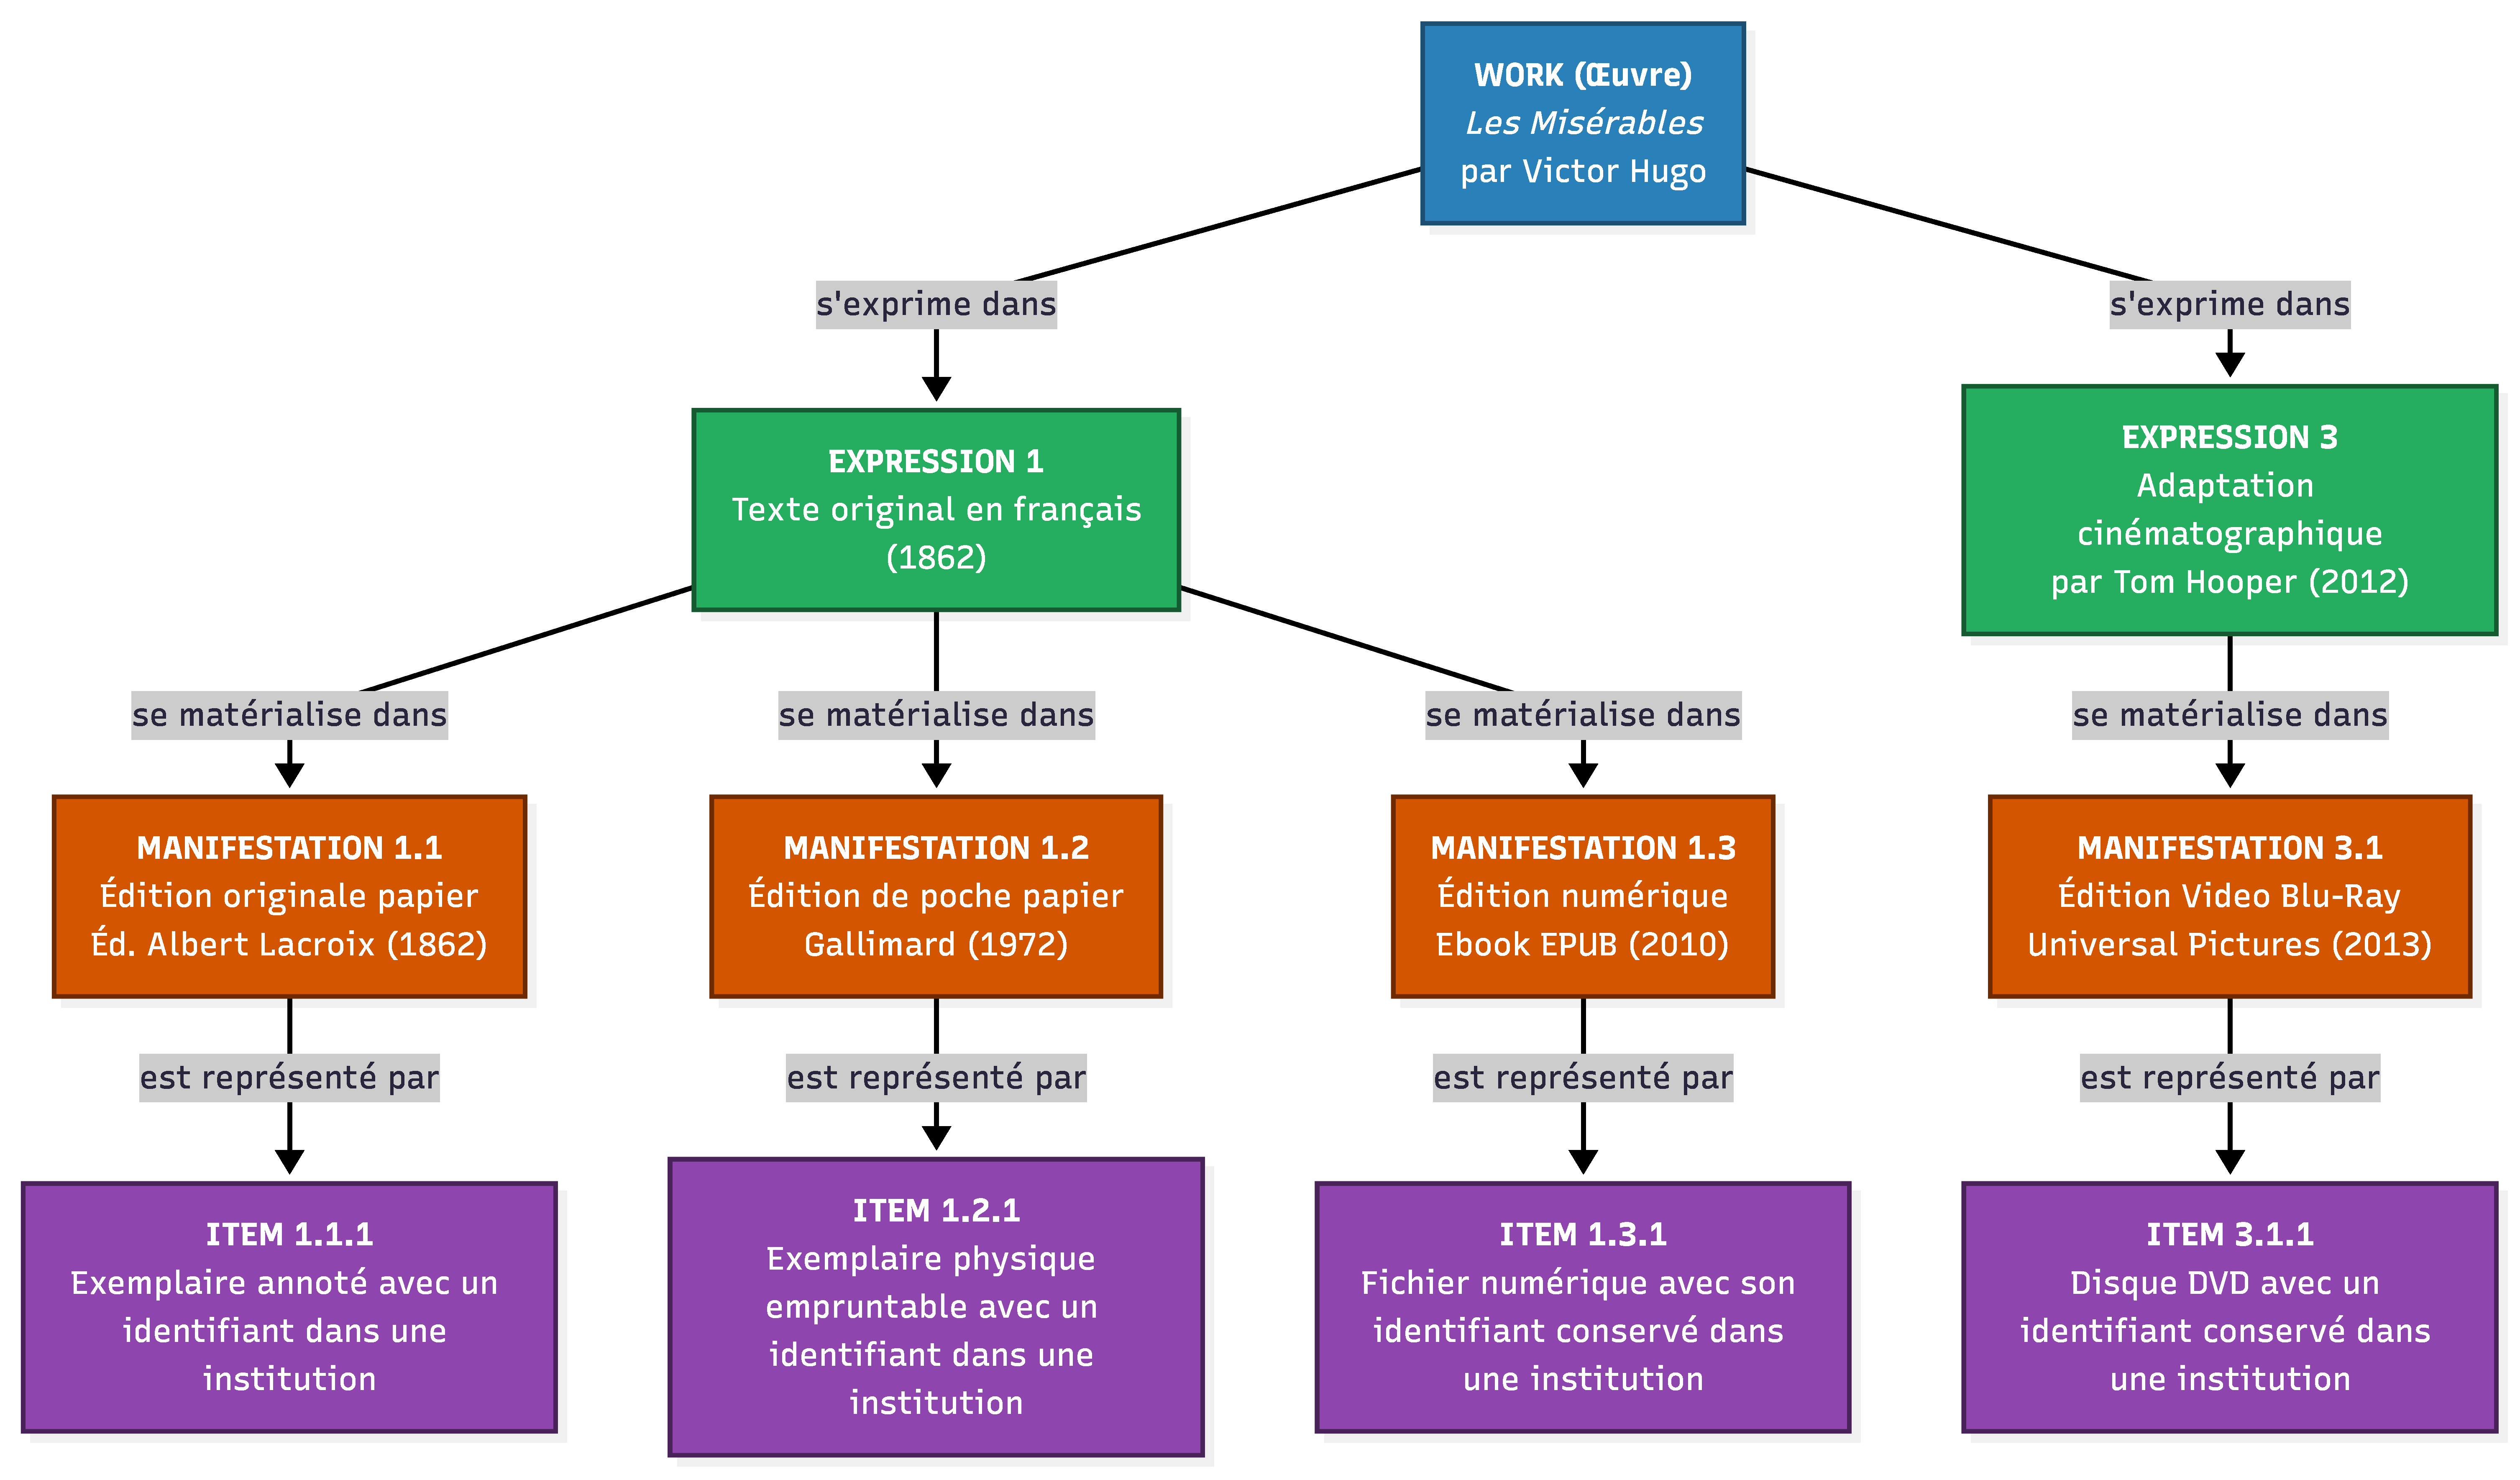
\includegraphics[width=0.9\textwidth]{./Schema/WEMI.pdf}
	\caption{Schéma d'un WEMI fictif d'une \gls{oe}.}
	\label{fig:wemiSimple_schema}
\end{figure}

Le second groupe est celui des personnes physiques et morales en lien avec chacun des niveaux \gls{WEMI} et parfois plusieurs \gls{WEMI}. 

Liée au niveau \gls{oe} elle en est la créatrice, celle qui a pensé l'idée intellectuelle. Liée au niveau \gls{exp} elle en est la réalisatrice, celle qui lui donne corps. Au niveau \gls{man}, elle en est la productrice responsable d'une forme générique qu'elle adopte. Et enfin, liée à l'\gls{it} elle en est la propriétaire. Notons que la créatrice peut aussi être réalisatrice, productrice et possesseuse au sein d'un même \gls{WEMI}. Ou alors créatrice dans un \gls{WEMI} et productrice dans un autre. Simplement, le lien avec un niveau \gls{WEMI} est toujours de même nature. \newline

Enfin, le troisième groupe est celui des éléments complémentaire au niveau \gls{oe} d'un \gls{WEMI}. on y retrouve les événements, les objets, les lieux ou les sujets qui servent donc à enrichir le niveau \gls{oe} afin de mieux l'indexer. Ce niveau peut être lié à plusieurs éléments de ce groupe et permet de créer des relations entre les \gls{oe} d'une même collection ou entre plusieurs collections. De cette manière, un utilisateur intéressé par un sujet précis peut obtenir plus de résultat à ses requêtes.\newline

De manière schématique, voilà ce que représente un \gls{WEMI} complet :

\begin{figure}[H]
	\centering
	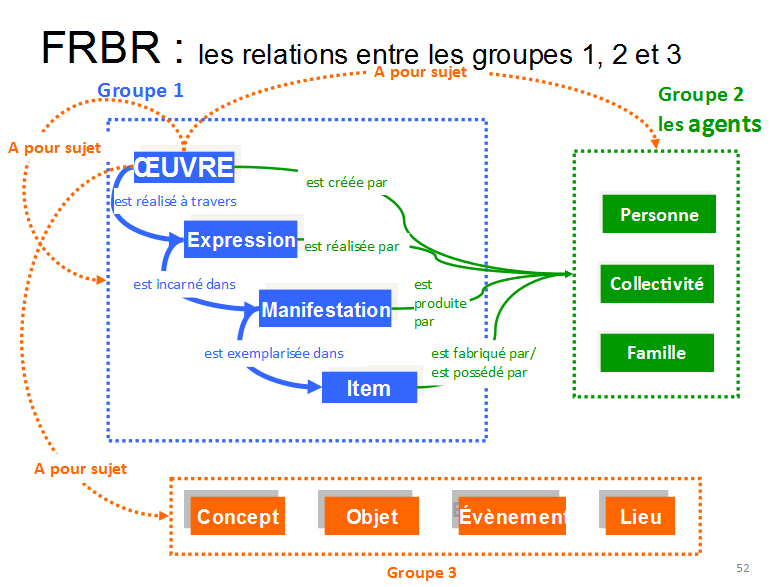
\includegraphics[width=0.7\textwidth]{./Schema/frbrComplet.png}
	\caption{Schéma de fonctionnement des liens dans un WEMI. Source : \url{https://mediadix.parisnanterre.fr/medias/fichier/catalogage-isbd-unimarc-apports-theorique-maj-2025_1736242651118-pdf}}
	\label{fig:wemiComplet_schema}
\end{figure}

Dans le cadre de l'\gls{imgani}, la \gls{FIAF} adapte ce modèle aux particularités de cette typologies. Notamment en modifiant la notion d'\gls{oe} et rajoutant celle de la \gls{vrt}.

Pour l'\gls{imgani}, l'\gls{oe} et l'\gls{exp} sont une seule et même entité.\footcite[p.21]{fairbairnManuelCatalogageImages} Ainsi, elle intègre également les circonstances de création originale de l'\gls{imgani}, des notions de temporalité, de localisation et de matérialité définies. Elle a également des relations différentes avec les personnes puisqu'elle est dotée d'une personne créatrice, mais aussi réalisatrice et productrice. Ajoutons à cela la diversité typologique importante de l'\gls{imgani} qui est incluse dans la notion d'\gls{oe} amenant à une fluctuation dans le niveau d'informations attendu.\newline

L'\gls{imgani} se caractérise également par son caractère évolutif. Outre les restaurations, elle peut être modifiée de multiples manières avant même son entrée dans une collection. Prenons l'exemple de la censure qui peut altérer la bande son, le montage ou encore l'intégrité visuelle de l'\gls{oe} impactant parfois le concept artistique exprimé. Sans constituer une \gls{oe} à part entière, elle n'est plus l'\gls{oe} originale exprimée dès la création artistique. Ainsi, la \gls{FIAF} crée une entité \gls{WEMI} unique : la \gls{vrt}.

On l'utilise dès lors qu'une modification impacte la description de l'\gls{imgani}. Que ce soit des ajouts ou des retraits de \glspl{sq}, \glspl{sc} ou \glspl{pl} ou bien des modifications dans sa production, dans les comédiens ou dans sa bande son comme par exemple un doublage.\footcite[p.23]{fairbairnManuelCatalogageImages}\newline

Ces particularités changent l'organisation du \gls{WEMI} de deux manières. D'abord sur le découpage structurel, puisque le niveau \gls{exp} disparaît laissant place à celui facultatif de la \gls{vrt}. Ensuite, sur la répartition des informations à indexer, puisque ces remaniements demandent de nouveaux points d'analyses à indexer. 

Le modèle \gls{WEMI} proposé par la \gls{FIAF} est surtout plus souple et ce décline en 4 modèles. Chacun présente une répartition différentes des informations. \footnote{Pour plus d'informations voir \cite[p.9 à 13]{fairbairnManuelCatalogageImages}} Nous n'allons pas tous les présenter ici afin de pouvoir nous attarder sur les choix effectués par SkinSoft.

\subsection{La gestion de l'\gls{imgani} dans l'application SkinSoft}

\label{S-Movies}

Dans le logiciel SkinSoft, la gestion des \gls{imgani} est réservée au module S-Movies. Nous ne reviendrons pas sur cette notion de module, déjà vue précédemment\footnote{Voir page \pageref{module}}. 

Ce qui distingue S-Movies des autres modules de la suite logicielle est sa gestion totalement transparente des niveaux \gls{WEMI}. Chaque entité \gls{WEMI} possède sa propre \gls{table}, donc ses propres données et points d'accès ce qui permet de bien cloisonner les niveaux \gls{WEMI} et de diriger l'utilisateur plus facilement entre ces derniers. La structure \gls{WEMI} adoptée est la suivante : \newpage

\begin{figure}[H]
	\centering
	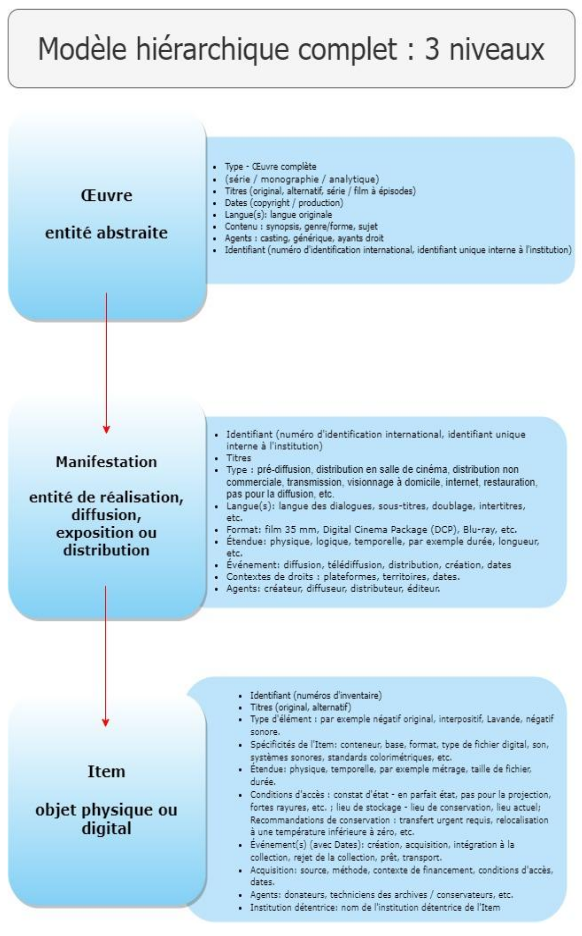
\includegraphics[width=0.8\textwidth]{./Schema/frbrSmovies.png}
	\caption{Schéma du modèle WEMI implanté dans la solution S-Movies. Source : \cite{fairbairnManuelCatalogageImages}}
	\label{fig:wemiSmovies_schema}
\end{figure}

La \gls{vrt} est considérée comme une \gls{man}. \footcite[p.23]{fairbairnManuelCatalogageImages} Ce choix vise à simplifier le parcours utilisateur en rendant son inclusion similaire à celle d'une \gls{man}, ne s'en distinguant que par un champ permettant de renseigner le type de \gls{vrt} dont il s'agit.

Les différents niveaux \gls{WEMI} sont connectés via des champ de lien créant une hiérarchie. Ils sont souples, modifiables à tout moment et multi-relationnels. Ainsi, la gestion des \glspl{imgani} reste fidèle aux principes de gestion proposés par la \gls{FIAF}\footnote{Voir \cite{fairbairnManuelCatalogageImages}}.\newline

Cette souplesse fait de S-Movies un logiciel permissif permettant à l'utilisateur d'adopter différents parcours afin d'effectuer les mêmes actions. Nous allons donc essayer de retracer un parcours utilisateur typique et privilégié, tout en énonçant les diverses possibilités s'ouvrant à lui.

L'utilisateur commence toujours par la création d'une notice \gls{oe} dans la \gls{table} dédiée, qui est également la page d'accueil de l'application. En fonction de sa configuration\footnote{Pour plus d'informations voir page \pageref{module}}, l'utilisateur peut rentrer manuellement une certaine quantité de données ce qui demande donc, en amont, une étape d'analyse afin de correctement distinguer où stocker l'information. Cette notice peut être liée à des archives, objets de musées ou des notices bibliographiques provenant des autres modules. Cela permet de créer des relations afin de circonscrire des univers cinématographiques entiers tout en gardant les spécificités de gestion de chaque objet.\newline

Ensuite, il peut créer une \gls{man} depuis la table dédiée ou une notice \gls{oe}. Si la création se fait depuis la table, elle peut être reliée à n'importe quelle \gls{oe}, et si elle est créée depuis une notice d'\gls{oe} elle y est automatiquement reliée. Peu importe la modalité, cette étape demande une analyse humaine afin de préciser la nature de la \gls{man}, notamment si c'est une \gls{vrt}. Cela demande donc une analyse effectuée au moment de la création du \gls{WEMI} et basée sur des connaissances cinématographiques. Notons qu'une \gls{man} peut être liée à plusieurs \oe{uvres}, comme les coffrets qui réunissent des \oe{uvres} différentes dans une même \gls{man}.\newline

Enfin, il peut créer un \gls{it}. Cette notice peut être créée en même temps qu'une notice d'entrée par exemple ou sous bien d'autre modalité, ce qui s'explique par le fait que c'est à ce niveau qu'on gère le \guillemet{cycle de vie} pensé par David Bearman.\footcite{ArchivesMuseumInformatics} Notons que plusieurs \gls{it} peuvent être liés à une seule \gls{man}.

\subsection{Complexité et limite de l'indexation des \glspl{imgani}}

Les \glspl{imgani} sont très riches en informations visuelles, parfois textuelle avec les crédits. Il faut donc pouvoir récupérer ces données, ce qui demandent des traitements différents puis les répartir sur les niveaux \gls{WEMI} appropriés. Dans les productions amatrices, les informations à indexer sont souvent uniquement visuelles ce qui demande d'analyser chaque \gls{oe} afin d'en extraire des mots-clés, des caractéristiques uniques, etc, ainsi que d'en déterminer le niveau \gls{WEMI} d'appartenance. 

Rajoutons également que l'indexation se complexifie avec la question de l'héritage des champs notamment pour la \gls{vrt}. En effet, une donnée portée par l'\gls{oe}, comme les comédiens, peut se retrouver invalide dans la \gls{vrt} en découlant. Cela peut créer une incohérence d'indexation et des difficultés de modifications de la donnée.\newline

\label{imganiExemple} Pour illustrer ces limites, prenons le cas d'une institution aux besoins de gestion spécifiques et utilisant S-Movies.\footnote{Pour des raisons de sécurité et de confidentialité, le nom de l'institution est anonymisé.} 

Certaines \glspl{imgani} ont été réunies sur un même support de conservations sans séparation entre les \gls{oe}. Deux problématiques en émergent : d'abord un \gls{WEMI} complexe, puisque plusieurs \glspl{oe} sont réunies en une seule \gls{man} d'où découle plusieurs \glspl{it}. De plus, le besoin de séparer matériellement dans l'application chaque bande vidéos et sonore de chaque \gls{it} afin de pouvoir les reconstituer dans des notices. 

Son schéma \gls{WEMI} est réalisable, mais toute l'étape de traitement est problématique. Il repose sur l'analyse de bobines entières, l'identification de chaque entités présentes et de leur association au segment de bobine concerné. Cependant, cela ne peut être fait que par l'humain à l'aide de logiciels de traitement externes spécialisé. De plus, il n'y a aucun crédit permettant des identifications de caractéristiques clés facilement. Après avoir segmenté les bobines en plusieurs \glspl{imgani}, il faut les analyser individuellement pour en extraire des informations clés. Ce qui peut être long, fastidieux et prompt aux erreurs humaines.\newline 

Cet exemple met en valeur les problématiques principales de l'indexation de cette typologie documentaire. SkinSoft cherche aujourd'hui à faire évoluer S-Movies pour proposer des modalités de gestions plus adaptées par le déploiement d'un outil d'indexation semi-automatisée notamment afin d'automatiser et homogénéiser les indexations. Ce serait un \textit{pipeline} basé sur l'\gls{IA} allant de l'intégration dans l'application d'une vidéo à son indexation, en passant par sa segmentation en différentes \glspl{imgani} indexées individuellement.

\newpage

\section[Outils et réalité technique]{Les différentes réalités de l’indexation semi-automatisée : focus sur l’image animées, un objet documentaire particulier.}

% !TeX root = ../document_maitre.tex

\label{réalitéIndexationAuto}

Ce processus est né de plusieurs constats sur l'indexation des textes, notamment, dans les bases de données patrimoniales. D'abord, l'indexation des textes et objets patrimoniaux par mots-clés, comme pratiquée encore aujourd'hui, permet d'optimiser l'interrogation des bases de données. Cependant, sur de grandes quantités de données procéder à une indexation manuelle, souvent effectuée par plusieurs personnes, amène à créer de la variation là où les bases ont besoins de constances. Ajoutons que plus la cohérence et la stabilité sont basses, plus les résultats sont imprécis.\footcite[p.1]{keversIndexationSemiautomatiqueTextes2009} 

Le second constat vient de la masse documentaire à traiter et de sa typologie. Les textes concernées concerne de vaste périodes chronologiques demandant la compréhension d'un vocabulaire vaste et évolutif et donc l'adaptation des mots clés. De plus, ces collections sont en expansion constante et toujours plus rapide, ce qui demande une augmentation du rythme d'indexation. \footcite[p.1]{keversIndexationSemiautomatiqueTextes2009}

Ces deux éléments mènent à penser que l'indexation par seul moyens humains devient une limite importante des bases de données patrimoniales qui, finalement, complexifie la tâches des \gls{SRI}\newline

Mais alors pourquoi une indexation \guillemet{semi-automatisée} et pas une totalement automatisée ? Si l'automatisation totale permet d'accélérer le traitement, on remarque des défaillances importantes. Ces processus ont tendances à produire les mêmes erreurs d'indexation que les humains tout en étant moins précis dans le choix des mots utilisés.\footcite[p.1]{keversIndexationSemiautomatiqueTextes2009}

Une indexation semi-automatisée permet de faire de l'\gls{IA} un outil d'appui, capable de suggérer des indexations et de proposer une base de travail propre très rapidement\footcite[p.69 à 71]{hussonIndexationIconographiqueIntelligence2025}. L'humain n'a plus à analyser chaque document lui même: il n'est plus que le vérificateur qui peut valider la proposition issus du processus ou alors créer une alternative. En associant la vérification humaine à la rapidité de traitement de l'\gls{IA}, on vise à augmenter la pertinence et la rapidité du processus. C'est ce que l'on l'appelle l'approche \textit{Humain in the loop} : l'\gls{IA} analyse et suggère, puis l’opérateur valide, invalide ou modifie.\newline

Avant d'examiner ce qui ce fait ou non dans le cadre de l'\gls{imgani}, commençons par l'analyse du principe appliqué à des collections de musées plus statiques. Pour cela, je m'appuierai principalement sur le projet mené par Pierre Husson\footcite{hussonIndexationIconographiqueIntelligence2025}, promotion TNAH 2025, au sein du projet \textit{IconographIA} consistant en l'application de tels processus sur des tableaux italiens du RETIF\footnote{Répertoire des tableaux italiens dans les collections publiques françaises}. 

Pierre Husson met tout d'abord en avant la complexité de notion de vocabulaire \footcite[p.9 à 17]{hussonIndexationIconographiqueIntelligence2025} qui est pluriel. D'abord car adapté à chaque typologie patrimoniale et ensuite car au sein même de ces typologies existent des subdivisions avec leurs propres besoins terminologiques. Ces vocabulaires sont standardisés et contrôlés dans des \gls{thesaurus} auxquels se rattacher comme ceux du Getty Research Institute. 

Bien qu'on puisse s'appuyer sur ces outils pour contrôler la génération d'un outil d'indexation automatique\footcite[p.38 à 40]{hussonIndexationIconographiqueIntelligence2025}, il existe un fossé entre la compréhension de ce que l'\gls{IA} voit et la sémantique des thésaurus. Pierre Husson met en avant que les modèles n'ont pas eu de difficultés des formes génériques \textit{(humains, animaux, épées, etc)}. Mais reconnaître que ces formes sont des concepts artistiques, comme des représentations codifiées consignées dans les \gls{thesaurus}, est encore hors de portée.\footcite{hussonIndexationIconographiqueIntelligence2025} Ils sont de plus imprécis face aux spécificités de l'art, notamment sur la question du genre iconographiques encore complexe à déterminée malgré de récent progrès.\footcite[p.41 à 43]{hussonIndexationIconographiqueIntelligence2025}

À la lumière de ces éléments, Pierre Husson conclut que l'indexation iconographique est loin d'être un processus automatisable. Cependant, les récentes avancées notamment avec les \gls{mmlts} capables de traiter texte, images, vidéos et/ou sons en même temps, permettent d'envisager de s'appuyer dessus dans des processus semi-automatisés. \newline

Mais alors, pourquoi faire de l'indexation semi-automatisée sur l'\gls{imgani} ? La raison principale est l'explosion quantitative des collection. La Cinémathèque française conserve à titre d'exemple plus de 40 000 \oe{uvres} cinématographique.\footnote{Pour plus d'information, consulter : \url{https://www.cinematheque.fr/les-collections-de-films.html}} Cela s'explique par l'intensification de la production de film professionnel : plus de 9511 films sont réalisés à l'échelle mondiale en 2023 contre 7620 en 2016 selon le WIPO\footnote{Pour plus d'informations, consulter : \url{https://www.wipo.int/fr/web/global-innovation-index/w/blogs/2025/global-film-production}}. Cela ne prend pas en compte la production de films amateurs, et toutes \glspl{imgani} produites en dehors du cinéma. De même, cela ne prend pas en compte ce qui est déjà produit et qui continu d'être conservée ce qui créer donc un véritable phénomène de masse demandant à accélérer le processus d'indexation.

Ajoutons à cela que, tout comme les tableaux, l'\gls{imgani} pose ses propres difficultés à commencer par la notion de mouvement. Pour créer cette impression de mouvement, une \oe{uvre} d'\gls{imgani} est composée de plusieurs centaines, ou milliers, d'images capturées à la chaîne pendant un instant déterminé. Ces images sont donc porteuse de sens, surtout au sein d'ensembles que sont les \glspl{sq} et les \glspl{sc}. L'indexation de vidéos ou de films entier repose donc principalement sur l'analyse de ces images au sein de ces deux ensembles qui déterminent un sens précis. 

De plus, bien que, comme pour les tableaux, on cherche à reconnaître les entités, les personnes, les objets, et tout autre éléments, mais dans cette notion d'ensemble, l'\gls{imgani} possède ses propres besoins d'indexation. En voici les trois principaux :

D'abord, celui d'une extraction automatique des \gls{sq} ou les \gls{sc} au sein d'une \oe{uvre}, Ou bien d'\oe{uvres} au sein d'un même support, afin de proposer une indexation optimale pour des résultats de recherches précis. Disposer d'un outil capable de découper automatiquement les \oe{uvres} d'\gls{imgani} en des unités documentaires plus petites et indexées à cette échelle est essentiel.

Un second besoin est de pouvoir faire des liens entre différentes \gls{sc} et/ou \gls{sq} d'une même \oe{uvre}, ou idéalement entre différentes \oe{uvres}. Cela peut permettre de reconstituer des arcs narratifs multiples ou encore de suivre l'évolution d'un sujet d'un bout à l'autre de l'\oe{uvre}. L'idée étant de pouvoir saisir la richesse des liens caractérisant les \oe{uvres} d'\gls{imgani}. Ils peuvent être faits entre les \oe{uvres}, au sein de suites thématiques comme les duologies la notion de saisons au sein d'une série. Saisir ces liens et porosités est aujourd'hui un objectif pour certaines institutions.

Enfin l'association entre le visuel et le son, une caractéristique principale des \glspl{imgani} aujourd'hui. L'idée est d'exploiter l'\oe{uvre} et les thèmes contenus à la fois visuellement et auditivement. Par exemple une \gls{sq} triste peut être identifiée par les changements colorimétriques et émotions des acteurs, mais aussi par l'environnement sonore et les dialogues. Cela sous-entends que le processus gagnerait à pouvoir \guillemet{comprendre} le son au sein de \glspl{sc} et \glspl{sq} afin de mieux exploiter les thèmes présents.

L'ensemble de ces éléments distingue clairement le traitement d'\glspl{imgani} de celui de tableaux. Bien que les éléments à extraire peuvent être les mêmes, les spécificités de l'\gls{imgani} en complexifient fortement la détection et l'analyse. Ce qui demande donc à penser à de nouveaux outils et processus de traitement.\newline

On peut dés lors distinguer deux phases essentielles de traitement pour l'\gls{imgani}. Une phase de \guillemet{pré-traitement} pour décomposer l'\oe{uvre} ou la bande vidéo analysée en autant d'entités que nécessaire que cela soit à l'échelle des \oe{oeuvres}, \glspl{sc} ou \glspl{sq}. Et une seconde phase de traitement pour reconnaître et identifier les éléments d'indexations par l'usage de termes conforme à au moins un Thésaurus. 

Après des recherches sur le sujet, un premier constat s'offre à nous. Il n'existe pas encore de solutions \gls{ops} permettant d'effectuer cette chaîne de traitement. Des outils existent afin de réaliser certaines tâches comprises dans le processus, comme la \gls{do}, mais ils n'ont encore jamais été rassemblés. Et du côté des solutions privées, certaines solutions à destinations du monde patrimonial existent et sont déjà utilisé. Cependant elles manquent de transparence ce qui fait que nous n'avons pas connaissance de la méthodologie appliqués, des outils utilisés et des compatibilités avec des standards de descriptions.

On peut citer Archipanion que les Archives fédérales Suisses utilisent à des fins de reconnaissance et d'extraction de métadonnées sur des images et vidéos. Cette institutions a indexée plus de 200h de vidéos de l'émission \textit{Ciné-Journal} Suisse.\footcite{ArchipanionPourCineJournal} L'article reste succint et nous n'avons pour information que l'extrait suivant : \guillemet{Grâce à sa fonction de recherche par contenu visuel, Archipanion permet, en les décrivant, de rechercher des scènes ou des textes figurant dans le fonds du Ciné-Journal suisse et de trouver ainsi des contenus de manière exploratoire [...] Outre la recherche textuelle par description, Archipanion permet aussi de trouver des contenus visuels similaires au sein de la collection.}. 

Sur le site d'Archipanion\footnote{Pour plus d'information, consulter : \url{https://www.archipanion.com/fr/}} voilà les conclusions que nous pouvons établir. Le processus établit agit sur chaque images à analyser individuellement, y compris au sien d'\gls{imgani}. En s'appuyant sur de la \gls{CV} ou bien des \gls{mmlts}, il semble y avoir un processus de \gls{Vecsion} : chaque image se voit attribuer une \gls{vcs} en fonction des entités, des lieux et du style général reconnus. Lorsqu'un utilisateur interroge ces documents, l'utilisateur décrit ce qu'il souhaite trouver, donc une scène ou une image, qui est transmise à l'\gls{IA}. Cette requête est transformée en \gls{vcs} qui sont comparés à ceux des \glspl{imgani} stockées. Plus des \gls{vcs} sont proches, plus il est probable qu'il existe une correspondance. 

Des questions subsistent. Les personnes sont-elles reconnues ? Qu'en est-il des réalisateurs et équipes techniques ? Qu'elle est la précision des métadonnées générées ? Il y'a-t-il une indexation de toute l'entière de l'\oe{uvre} d'\gls{imgani} ou juste chaque image ? 



							% A REPRENDRE ICI 



L'opacité des solutions privées ne nous permet pas d'apporter des réponses à ces questions. Et les articles d'institutions utilisant cette solution ne sont pas nombreux, en réalité seul celui-ci semble exister ce qui peut s'expliquer par le caractèr récent de tels outils. Nous pouvons cependant déterminés deux choses : dans les deux sources, il n'y aucune mention de reconnaissance précises d'entités nommées. Une actrice célèbre, un monument ou encore un objet unique et identifiable ne semble être identifier suffisament précisément afin de l'indexer de cette manière. Les analyses semblent rester très générales : une voiture, une femme, un homme, etc. Ensuite, il n'y aucune mention de reconnaissance de l'architecture documentaire. Par exemple, une bobine comportant 3 \gls{oe} différentes semble être analysées comme une seule et même \gls{oe} ce qui ne permet de corriger un problème de mélange des supports et des \gls{oe} rencontrées par les institutions sur cette typologie. 

Finalement, c'est une solution assez générale appliquant des principes déjà éprouvées sur les images fixes à des objets en mouvements. L'\gls{imgani} semble être confondu avec une image statique, et est donc analysée de la même manière ce qui amène à perdre la richesse amenée par cette typologie documentaire. De plus, traiter chaque \gls{imgani} composant une \oe{uvre} représente un processus long et coûteux qui, appliqué à des collections comme celles de la Cinémathèque française, peut ne pas présenter un rapport coûts / bénéfices suffisant. \newline

Du côté des solutions dites \textit{open source}, le seul processus de traitement des \gls{imgani} connu est \textit{vitrivr-engine}\footnote{Pour plus d'informations, consulter le github du projet : \url{https://github.com/vitrivr}} développé par l'Université de Bâle, en Suisse, et sur lequel est basé la solution Archipanion. 

Cette solution est basée sur la recherche de contenu, c'est à dire qu'on offre la capacité à l'utilisateur de décrire ce qu'il recherche et de l'orienter vers le bon passage d'une vidéo.\footcite{rossettoVitrivrFlexibleRetrieval2016} 

Son architecture est modulaire, c'est à dire qu'elle se compose, ici, de 3 briques logicielles qui intéragissent ensemble mais qui ne composent pas un outil unique. Une interface d'interrogation, \textit{vitrivr-ng}, une base de donnée, \textit{Cottontail DB}, et un logiciel multimodal pour la recherche dans des documents multimédia, \textit{Cineast}. Voici un schéma du fonctionnement global applicatif : 

\begin{figure}[H]
	\centering
	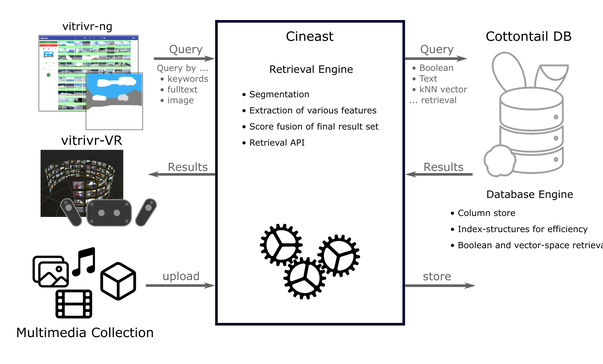
\includegraphics[width=1\textwidth]{./Schema/vitrivr.png}
	\caption{Schéma de fonctionnement de la solution vitrivr. Source : site officiel vitrivr à l'URL \url{https://vitrivr.org/vitrivr.html}.}
	\label{fig:vitrivr_fonction}
\end{figure}

Le logiciel fonctionne sur deux étapes. La première étape est celles de prétraitement des données : à l'intégration des documents multimédias dans la base de données, cela passe par \textit{Cineast} qui analyse l'\gls{imgani}, en extrait les entités visibles et lui donne un \gls{vcs} associé. La base de donnée stocke à la fois les \oe{uvres} multimédias et leurs représentations vectorielles au sein d'une base PostGreSQL adapté au stockage vectoriel \footcite{rossettoVitrivrFlexibleRetrieval2016}. La seconde étape est celle de l'interrogation utilisateurs : la requête peut être formulée de différentes manière, par phrase, par recherche de similarité avec une image ou un schémas\footcite{rossettoVitrivrFlexibleRetrieval2016}, et est d'abord vectorisée par \textit{Cineast} avant d'être envoyée à la base de données par une API. Les \gls{vcs} sont ensuite comparés, et les résultats sont renvoyés à l'utilisateur soit directement dans l'interface \textit{vitrivr-ng} soit en format 3D via \textit{vitrivr-VR}.  

Ce qui est intéressant, c'est l'absence des différentes modalités d'interrogations des documents multimédias dans la solution de Archipanion. En effet, seule la recherche par requête textuelle ou par mots-clés semble intégrée. Destinée à la gestion des collections, on peut penser que l'approche par schéma et images similaires ait été jugée non ou peu pertinente notamment dans des questions d'usages et de pratiques. 

Finalement, nous nous retrouvons un peu face aux mêmes limites pour une intégration dans le monde patrimonial. Ce logiciel est concentré sur le contenu, le visuel, mais délaisse l'aspect documentaire. Les \gls{imgani} sont annotées, identifiées, mais elles ne sont pas indexées, mises en relations, décortiquée et encore moins manipuler comme un objet patrimonial. Une institution patrimoniale avec des besoins fort en matière de gestion risque de se trouver limitée : pas d'identification des personnes, pas d'identification technique, pas de rédaction d'une notice, pas de séparation en \glspl{sc} ou \glspl{sq} ou même entre \oe{uvres}.

Nous pouvons donc conclure que les solutions proposées pour la gestion de l'\gls{imgani} par \gls{IA} sont orientées gestion des contenus et non gestion documentaires. C'est insuffisant lorsque l'on souhaite gérer une collection patrimoniale. \newline

Cela nous amène donc à voir plus large que des solutions sur étagères afin de trouver des outils permettant de répondre à l'ensemble des besoins institutionnels. Nous allons donc présenter des outils \textit{open-source} qui, articulé ensemble, peuvent amener à penser et créer une solution d'indexation complète de l'\gls{imgani}. 

\subsection{Manipulation de l'image et des \glspl{pl}}

Le premier élément est le besoin de manipulations des documents multimédias en tant que tel. Une institution patrimoniale peut souhaiter séparer différentes \oe{uvres} d'\gls{imgani} présentes sur un même support physique, ou bien une même \oe{uvres} en différentes sous-unités que sont la \gls{sc} et la \gls{sq}. Cela demande nécessairement de pouvoir manipuler le document multimédia afin de le découper à des endroits précis et de pouvoir placer des repères temporels sur ces découpages. De cette manière, on pourrait segmenter une bande vidéo en différent segments indépendant avec chacun un \guillemet{horodatage}, c'est à dire un marqueur temporel au début et à la fin du segment afin de le situer à l'échelle de l'\oe{uvre} originale. 

\label{FFmpeg}Pour cela, il existe le logiciel FFmpeg qui permet de manipuler des bandes vidéos et des bandes sons. Logiciel \textit{open-source} pouvant traiter tous les formats vidéos et audios, il est très utilisé par des plateformes multimédia comme Youtube afin de permettre de manipuler les vidéos \textit{(diffusion, manipulation du flux, etc)}. Le gros avantage de ce logiciel est sa compatibilité avec des langages de programmation comme python, qui permettent de l'intégrer dans des workflows automatisés de traitement de données assez facilement.\footnote{Pour plus d'informations, consulter : \url{https://www.ffmpeg.org/documentation.html}}\newline

Avec FFmpeg, la \gls{seg} audio et vidéos est rendue possible. Autrement dit, on peut créer un extrait d' une \oe{uvre} avec la granularité désirée. Cependant, FFmpeg demande une action humaine : il n'intègre pas de système afin de repérer des variations justifiant un découpage. \label{PyScene}L'outil PySceneDetect permet d'identifier dans une piste vidéos chaque changement de \glspl{pl}. Il fonctionne selon le principe de \textit{threshold} c'est à dire que l'utilisateur définit un palier indiquant au logiciel que toute comparaison entre image produisant un score inférieur à ce palier signifie que c'est un seul \gls{pl}. Si le score de comparaison y est supérieur, alors ce sont des \glspl{pl} différents. \footnote{Pour plus d'informations, consulter : \url{https://www.scenedetect.com/}} 

Cet outil est très intéressant : d'abord c'est une librairie python ce qui le rend parfaitement intégrable à un script automatique. On peut ainsi lier FFmpeg à PySceneDetect afin de lier la détection à l'extraction. De plus, il s'appuis sur d'autres librairie python reconnues et approuvées pour l'analyse d'image. On peut notamment penser à OpenCV, MoviePY et PyAV pour l'analyse images par images dans une vidéo ou bien d'images fixes. Ce sont des solutions très souples permettant de choisir un détecteur, c'est à dire un algorithme qui permet d'analyser une image et de la comparer avec l'image suivante afin de déterminer si il y a un changement de \gls{pl} ou non. Chaque détecteur est spécialisé sur l'analyse d'un composant de l'image, par exemple : \footnote{Pour consulter la documentation relative à chaque détecteur, consulter : \url{https://www.scenedetect.com/docs/latest/api/detectors.html}} \label{detecteurs}

\begin{enumerate}
	\item \textit{ContentDetector} : ce détecteur est le plus utilisé car le plus complet et souple. Chaque image est analysées dans son contenu notamment colorimétrique et structurel et obtient un score de détection. En fonction de cette analyse, il calcule un score pour chaque image, disons une forme de \gls{vcs}, et compare les score entre eux. La différence entre les scores est ensuite reportée au \textit{threshold}.
	\item \textit{AdaptiveDetector} : ce détecteur reprend le principe précédent. Il analyse les mêmes points, de la même manière. Le changement opère au niveau du système de comparaison. En effet, au lieu de se référer au \textit{threshold} ce détecteur calcule lui même une moyenne glissante entre les images. C'est à dire que le \textit{threshold} change automatiquement en fonction du cas présent. Cela rend le détecteur moins sensible aux mouvement de caméras, qui n'indique pas un changement de plan nécessairement. 
	\item \textit{TresholdDetector} : si les deux détecteurs précédents sont basé sur des analyses structurelles afin de repérer des coupures, celui ci s'attarde sur les pixels afin de repérer les changements plus fins comme des transitions. 
	\item \textit{HistogramDetector} : à l'échelle d'une vidéo, l'\gls{hist} est un graphique permettant de visualiser, et parfois gérer, l'équilibre entre ombres et lumières. Ce détecteur analyse cet histogramme, et compares les histogrammes des images afin de détecter des changements d'équilibre. Efficace afin d'identifier les coupures rapides. 
	\item \textit{HashDetector }: il est similaire à \textit{ContentDetector} et \textit{AdaptativeDetector} si ce n'est qu'il se base sur la création d'un \textit{hash}, c'est à dire une empreinte de taille fixe et propre à chaque image, pour chaque image. Ensuite, les \textit{hash} sont comparés et leurs écarts calculés puis mis en relation avec le \textit{threshold}\newline
\end{enumerate}

Ces détecteurs peuvent s'accumuler, permettant ainsi des analyses multiples mais alourdissant fortement le processus. Plus il y a de détecteurs, plus le traitement s'alourdis et plus on multiplie la finesse de l'analyse ce qui peut amener à faire de chaque petites variations une raison suffisante pour segmenter. 

L'extraction se fait à l'échelle du plan puisque cet outil repère les ruptures de prises de vues ce qui caractérise les différents \glspl{pl}. Les \glspl{sc} et \glspl{sq}, beaucoup plus intéressantes pour une institutions patrimoniales, ne sont pas encore saisisables par des solutions informatiques. Il est cependant tout à fait possible d'utiliser cet outil pour découper une \oe{uvre} en autant de \glspl{sc} et \glspl{sq} qui la compose. Commençons d'abord par définir ce qu'est \gls{sc} puis une \gls{sq}

Une \gls{sc} représente l'unité de base d'une \oe{uvre} d'\gls{imgani}. Il s'agit d'un ensemble de plans mettant en scènes les mêmes acteurs, dans les même lieux, souvent autour des mêmes objets et toujours autours des mêmes actions, sujets et objectifs. Ainsi, pour recréer une \gls{sc} il faut pouvoir identifier ces éléments de continuité au sein de \glspl{pl} adjacent et cela jusqu'à l'identification d'une rupture nette. Si nous sommes capables d'identifier ces éléments, on peut tout à fait penser à créer des \gls{vcs} pour chaque plan basé sur l'identification de ces éléments. Comme dans un système de \guillemet{recherche augmentée}, c'est la comparaison entre les \gls{vcs} qui va déterminer l'action et le résultat à retourner. Si au sein de \gls{pl} adjacents les \gls{vcs} sont extrêmement proche alors ils peuvent regroupé en une \gls{sc} et cela jusqu'à détecter une rupture avec un autre \gls{pl}.

Une \gls{sq} est un ensemble de \glspl{sc} regroupées autour d'éléments bien plus abstrait. Ces \glspl{sc} partagent une thématique commune, un sujet qui bien souvent sert au développement d'une partie de l'intrigue de l'\gls{oe}. En arrivant à saisir un motif, sujet ou thème commun il serait possible d'agir de la même manière que précédemment : vectoriser les \glspl{sc} sur ces éléments et rassembler les \gls{vcs} proches en \glspl{sq}. \newline

Ainsi on comprends que pour indexer une \oe{uvre} d'\gls{imgani} il faut aller bien plus loin dans le processus de traitement que la simple détection de plan autrement dit de rupture visuelle. Il faut pouvoir identifier des acteurs, et leurs apparitions dans les plans successif. Mais aussi reconnaître ou du moins caractériser en partie les lieux, parfois fictif, qui permettent d'ancrer l'action dans un élément \guillemet{concret}. En allant plus loin, il faut également des outils capable de déterminer la thématique générale des \glspl{pl} : dramatique, comique, action, etc. Ce n'est qu'a l'aide de ces éléments on peut envisager deux choses : indexer des éléments d'une \oe{uvre} et utiliser ces éléments pour créer des regroupements de \glspl{pl}.

Nous allons donc présenter des outils intégrable dans un script d'automatisation de l'indexation d'\glspl{imgani} permettant la détection et l'analyse des éléments identifiés. Comme nous l'avons déjà abordé, nous ferons l'impasse sur \newline le module \textit{Cineast} de \textit{Vitrivr}. Gardons simplement à l'esprit que ce module ne propose pas une indexation assez fine et précise et que de plus, l'\gls{imgani} est traitée comme une image fixe. Débutons par l'outil \textit{SAM 2}\footcite{SAM2Segment} et son \textit{framework} dérivé \textit{Seg2Track-SAM2}\footcite{mendoncaSeg2TrackSAM2SAM2basedMultiobject2025a}.

\subsection{\Gls{seg} d'une \gls{imgani}}

\label{SAM2} Développé par l'entreprise Meta, \textit{SAM 2} est un modèle d'\gls{IA} spécialisé en \gls{CV} afin de segmenter une image ou une vidéo : c'est à dire de détecter et isoler tout élément composant une image. Ce modèle est particulièrement intéressant pour trois spécificités : 

D'abord sa capacité de \textit{zero-shot}, c'est à dire sans être entraîné à détecter un objet spécifique, il pourra tout de même le segmenter au sein d'une image. \footcite[p.8 à 10]{raviSAM2SEGMENT2025}

Ensuite, sa capacité à recevoir des \textit{prompts} de la part de l'utilisateur, ce qui permet deux choses : de mieux diriger la \gls{seg} et de la réitérer si nécessaire dans un but d'affinage. \footcite[p.3 à 4]{raviSAM2SEGMENT2025}

Enfin, son système de mémorisation des formes détectées. Dans une \oe{uvre} d'\gls{imgani} il n'est pas rare qu'un objet soit totalement visible puis ensuite peu à peu caché par un autre élément. Ce modèle mémorise ce qu'il détecte, de cette manière si l'objet détecté est partiellement couvert à un moment donné, le modèle garde la forme initiale de l'objet. C'est particulièrement utile afin de traquer les objets. \footcites[p.4 à 5]{raviSAM2SEGMENT2025}{SAM2Segment}

Cependant, cet outil possède trois limites importantes. La première est l'absence d'une attribution et d'une gestion d'identité à des objets. Un objet détecté est gardé en mémoire, ainsi si il disparaît partiellement de l'image le modèle garde en mémoire son emplacement et sa forme. Cependant, comme il n'est pas identifié si cet objet disparaît puis réapparaît, \textit{SAM 2} le reconnaît comme un nouvel objet ce qui est faux. Appliquée à des institutions patrimoniales, l'absence de cette identification risque de poser deux problèmes : d'abord car le modèle risque de détecter constamment le même objet, et ensuite car cela complexifie la reconnaissance d'un même objet dans différentes \glspl{sq} ou \glspl{sc}. La seconde est la mise en mémoire en elle même car sur une volumétrie importante, le nombre d'objets à détecter est exponentiel ce qui alourdit la mémoire du modèle et en ralentit le traitement.\footcite[p.22 à 40]{raviSAM2SEGMENT2025} La dernière limite est l'absence de classification des objets. En effet, \textit{SAM 2} reconnaît des formes mais ne pourra pas déterminer que ceci est une voiture et ceci un vase. C'est ce que l'on appelle un modèle \guillemet{classe-agnostic} \newline

\textit{Seg2Track-SAM2} permet d'apporter quelques solutions. Cet outil est un framework permettant d'associer \textit{SAM 2} à un modèle de reconnaissance d'objet pré-entraîné comme YOLO ou bien Faster R-CNN et au module \textit{Seg2Track} qui s'occupe de gérer l'attribution et la mise en mémoire d'identifiant des objets.\footcite{mendoncaSeg2TrackSAM2SAM2basedMultiobject2025a}

L'association à un modèle de reconnaissance d'objet externe, choisi par l'institution, permet de spécialiser le \textit{framework} pour la détection de certains objets et en déterminer la nature. Ainsi on brise la nature \guillemet{classe-agnostic} de \textit{SAM 2} en apportant, par une ressource extérieure, la possibilité d'identifier des classes d'objets comme des voitures, des vases, etc. Au-delà, cela permet d'accélérer le traitement et de le fiabiliser par l'application de deux modèles. \textit{SAM 2} est surtout utilisé afin d'assurer le suivi de l'objet au travers des différents \glspl{pl} se succédant. Le module \textit{Seg2Track} permet de résoudre l'attribution d'identifiant à chaque objet identifié. En effet, ce module permet d'attribuer un identifiant à chaque objet identifié, de le garder en mémoire et de l'associer à la forme de l'objet détecté elle aussi mémorisée, et ainsi de pouvoir reconnaître si le \guillemet{nouvel objet} détecté est bien un nouvel objet ou un même objet. 

Ce \textit{framework} se place aujourd'hui comme une référence dans la segmentation d'images et d'\glspl{imgani}. Sur le jeu de données KITTI MOTS du \textit{benchmarks} KITTI, ce \textit{framework} s'est placé 4ème en 2025 sur l'analyse de ce dernier, essentiellement composé de voitures et de piétons, sans entraînement préalable. \footcite[p.5]{mendoncaSeg2TrackSAM2SAM2basedMultiobject2025a} Dans un tout autre domaine, celui de la chirurgie, ce \textit{framework} a montré des résultats prometteurs sur la \gls{seg} multi-objets en \textit{zero shot} avec notamment une possibilité de \gls{ft} en temps réel permettant de réellement fiabiliser les résultats. \footnote{Pour plus d'informations sur le sujet, voir : \footcite{yuanSystematicEvaluationGuidelines2026}} \newline

Dans l'indexation d'une \gls{imgani}, disposer d'un tel outil est pertinent. Parfois chargée en informations visuelle, l'application de \textit{SAM 2} ou du \textit{framework} \textit{Seg2Track-SAM2} permettrait de faire un tri informationnelle via une \gls{seg} de l'image. Chaque objets et personnes pouvant être détectés et isolés les uns des autres tout en étant suivis au fur et à mesure des images composant l'\oe{uvre} analysée. \newline

\subsection{La compréhension des sous-titres}

Un autre élément pouvant être analysé pour indexation ce sont les sous-titres. Ils peuvent servir d'appui afin d'extraire du sens au sein d'une \gls{sc} ou \gls{sq}. Des outils comme VideOCR\footnote{Pour plus d'informations, consulter : \url{https://github.com/timminator/VideOCR}} sont spécialisés sur le sujet et permettent d'isoler les sous-titres de l'image, et de les transcrire en chaînes de caractères brutes pouvant ensuite être interprétée soit par l'humain soit par un \gls{LLM}.

Cependant cet outil a une limite importante. En effet, il ne repère pas automatiquement la zone de sous-titres et demande une intervention humaine : il doit désigner où ce situe cette zone à l'aide de son curseur. Il est pertinent de laisser cette possibilité à l'utilisateur : le texte n'est pas uniquement présent dans les sous-titres mais peut aussi l'être dans l'image en elle-même et il faut pouvoir contraindre l'analyse afin d'éviter tout mélange d'informations. De plus, la zone de sous-titres à une position variable : en fonction des dimensions de l'\gls{imgani} et de sa conception, cette zone peut varier en taille et en localisation. Ainsi, sur un grand jeu de données, cela offre une performance assez limitée puisqu'il faudrait définir à chaque fois la zone à traiter. \newline

\subsection{La reconnaissance de lieux et de personnes}

L'indexation demande de reconnaître des éléments tels des acteurs ou des lieux de manière précise. Commençons par l'indexation des lieux : 

La reconnaissance des lieux est une thématique assez massivement traitée. En effet, les institutions conservatrices ont assez rapidement exprimé le souhait de pouvoir géolocaliser des prises de vues photographiques à partir d'une analyse. Cette capacité à alors été conférée à des modèles d'\gls{IA} qui, à partir d'images peuvent estimer une géolocalisation : c'est la géolocalisation visuelle. Domaine à part entière en \gls{IA}, elle est composée d'outils et de réalités multiples. 

À l'origine, la géolocalisation visuelle à été développée pour les images fixes et donc les algorithmes, modèles et outils répondent aux besoins de ces derniers. On peut penser à l'outil \textit{PIGEON}\footnote{Pour plus d'informations, consulter le github : \url{https://lukashaas.github.io/PIGEON-CVPR24/}}, développé en 2023 et entraîné afin de surpasser l'humain sur le jeu \textit{Geoguesser} dans lequel il s'agit d'estimer une géolocalisation à partir de simples images fixes à 360°. Cet outil extrait des éléments clés de l'image, les analyse et estime à partir de ces derniers une localisation géographique. \footcite{haasPIGEONPredictingImage2023} Pour cela, il est entraîné sur un corpus de plus de 4 millions d'images et possède son propre moteur de découpage géographique permettant d'estimer des positions avec une marge d'erreur d'environ 25 kilomètres. 

Cependant, cet outil est également limité. D'abord, les analyses successives ralentissent le processus et le rendent de plus en plus coûteux. De plus, ce modèle n'est pas public : en effet, pouvant estimer des positions très précises il a été souligné que cela comporte un véritable risque de sécurité. Pour cela, il n'est destiné qu'à des usages académiques contrôlés, ce qui échappe à notre domaine d'application.\footcite[p.11]{haasPIGEONPredictingImage2023}. 

C'est aussi un outil inadapté à l'\gls{imgani}. En effet, il traite des images fixes sans notions d'ensemble d'images. On sait, par définition, qu'une \gls{sc} est constituée d'une succession d'images pouvant faire figurer le même lieu, parfois sous des angles différents. Cela implique donc deux limites : d'abord l'analyse de chaque image ou chaque plan ce qui, à l'échelle d'une \gls{sc}, constitue une tâche répétitive et coûteuse. Et de plus, en fonction du plan la prédiction du modèle peut varier : il n'est pas capable de comprendre qu'il s'agit simplement d'un autre angle et non d'un nouveau lieu.\footcite[p.1 à 2]{gargSeqNetLearningDescriptors2021} \newline

L'application de la géolocalisation visuelle sur l'\gls{imgani} est relativement récente. L'avancée majeure est de prendre en compte cette notion d'ensemble d'images et donc de repérer différents éléments à plusieurs moments d'une même \gls{sc}. Cela présente deux avantages : réduire la fréquence d'analyse en n'analysant non pas toutes les images mais uniquement certaines, et éviter les erreurs de prédictions. Deux outils y répondent, chacun avec leurs avantages et inconvénients : 

D'abord \textit{SeqNet}, un modèle d'\gls{IA} basé sur un \gls{CNN}. Il prend en entrée un extrait vidéo et y récupère des \guillemet{échantillons} de vidéos répartis sur toute la durée de l'extrait. L'avancée majeure est qu'ils sont analysés individuellement puis réunis afin de donner lieux à une prédiction unique qui s'applique donc à l'ensemble de l'extrait.\footcite{gargSeqNetLearningDescriptors2021} 

Ce modèle présente deux limites majeures : sa sensibilité à la taille des extraits fournis, qui doivent avoir une durée et un nombre d'images fixe, et à la continuité visuelle dans ces mêmes extraits. En effet, le modèle attend d'avoir des extraits de taille fixe, avec un nombre d'image fixe et sans variations importantes en terme de plans et de lumière ce qui ne correspond à la réalité des \oe{uvres} conservées.

Un second outil est \textit{Video Swin Transformer}\footcite{liuVideoSwinTransformer2021}. L'innovation réside ici dans le passage de l'utilisation d'une architecture \gls{CNN} à une architecture de \gls{tfmrs}. Sans rentrer dans les détails techniques, ce modèle reprend les innovations apportées par \textit{SeqNet} et, grâce à un changement d'architecture, y apporte de l'\gls{autat} appliquée à la 3D ce que \textit{SeqNet} n'intègre pas. De cette manière, le modèle devient moins sensible aux différentes variations visuelles qu'il peut y avoir, tant qu'il ne s'agit pas d'un changement de lieu, et moins sensibles aux variations de durées et de nombre d'images dans un extrait. 

Cependant, il existe de nombreuses limites. La première est le coût en ressources : en effet, l'analyse d'éléments en 3D demande d'importantes capacités en \gls{GPU} ce qui est cher. De plus, on observe une perte de performance croissante en fonction de la taille des extraits : plus l'extrait est long, plus il contient d'images et moins le modèle est efficace. Enfin, le modèle nécessite un pré-entraînement et est très dépendant des données fournies à ce moment là. En effet, il ne possède pas de capacité \gls{zsht} ce qui limite très fortement son champ d'application notamment sur des données patrimoniales. \newline

Finalement, le domaine de la géolocalisation visuelle est actuellement en pleine mutation. L'arrivée des \gls{VLM} et de la diversité des modèles d'architecture d'\gls{IA} amènent de nouvelles innovations et de nouveaux outils toujours plus légers, rapides et moins coûteux. Cela reste cependant un domaine peu appliqué aux \glspl{imgani}, ce qui amène à questionner la faisabilité d'indexer automatiquement les lieux figurant dans des \oe{uvres}. 

L'indexation des acteurs et actrices est elle aussi complexe car composée de différentes réalités. Dans un film professionnel par exemple, les acteurs et membres de l'équipe techniques sont répertoriés dans ce que l'on appelle des crédits : ces images avec uniquement du texte présentant la liste des acteurs, actrices et membres des équipes techniques. Cependant, dans un film amateur ce n'est pas la même réalité : les personnes sont souvent inconnues et surtout il n'y a pas de crédit. Imaginons une vidéo amateur sur laquelle figure une personne célèbre, il n'y aura pas de crédit pour l'indiquer. 

Il est difficile d'indiquer quel cas est le plus rencontré dans les institutions conservatrices car tout dépend de la typologie de leurs fonds. Ainsi, nous allons présenter deux outils correspondant aujourd'hui à ce qu'il est possible de réaliser dans ce domaine. \newline

Commençons par les films professionnels. Pour cela, il faut pouvoir repérer les images dites de crédits, en extraire les chaînes de caractère et en analyser le contenu sémantique afin de l'indexer dans les bons champs. Aucun outil ne permet de réaliser les 3 tâches en un seul temps, ce qui constitue un des points de tensions entre le besoin des institutions conservatrices et ce que proposent les solutions d'indexation d'\glspl{imgani} actuelles. Cependant, cela ne signifie pas qu'il n'existe pas de solution. Nous traiterons cela plus en détail par la suite, mais présentons trois outils pouvant être combinés afin de répondre au besoin. 

Tout d'abord, il s'agit de pouvoir identifier et extraire les \glspl{imgani} sur lesquelles figurent les crédits ou non. Ils se distinguent de la majorité des autres images composant un film par leur fonds noirs, et le texte blanc réparti en général sur une seule colonne et défilant sur plusieurs minutes. Pour cela, des algorithmes de \gls{CV} comme ce qui est faisable avec \textit{OpenCV} peuvent permettre de les reconnaître et de les isoler du reste de l'\oe{uvre}. En effet, cette librairie python est très souple : elle permet de segmenter une image, comme de la manipuler ou bien encore de les analyser. Cette analyse se fait sans appui sur du \gls{DPL} et se base sur une analyse structurelle comme nous l'avons vu avec la question des détecteurs de \textit{PySceneDetect} \footnote{Voir page \pageref{detecteurs}}\newline

Ensuite, il s'agit de pouvoir extraire l’information écrite dans l'image. Bien que les crédits tendent aujourd'hui à se diversifier dans la police d'écriture et leur organisation, cela reste plutôt stable. Et on peut penser que pour une institution conservatrice conservant des films relativement \guillemet{ancien}, la stabilité est encore plus grande. Il faut ainsi un modèle d'\gls{OCR} qui sera capable de reconnaître dans l'image le texte et de l'extraire sous forme de chaîne de caractères brutes. Des outils comme \textit{Tesseract} ou \textit{Kraken} qui sont \gls{ops} peuvent permettre cette extraction brute. 

Cependant, à ce stade nous n'avons pas de compréhension sémantique. D'autant plus que les crédits sont faits de deux manières : pour le casting, nous avons d'un côté le nom de l'actrice et de l'autre côté son rôle, et pour l'équipe technique, des catégories avec des listes de noms sous formes de paragraphes ou bien de liste. Le risque ici est de ne pas réussir à associer l'actrice à son rôle, et de considérer le rôle comme étant une personne réelle à indexer, et de ne pas associer les membres des équipes techniques à leur bon rôle. Pour cela, le \gls{LLM} constitue un bon outil d'analyse afin de réorganiser l’information. A l'aide de sa capacité de \guillemet{compréhension} du langage naturel et grâce à sa capacité d'analyse, le \gls{LLM} peut très bien réorganiser l’information. \newline

\label{FaceNet} Pour les films amateurs, ou plutôt dénués de crédits, il faut envisager de nouveaux outils permettant de reconnaître l'identité des personnes souhaitées. C'est le cas de \textit{FaceNet} développé par Google qui permet de reconnaître des personnes grâce à son modèle d'\gls{IA} basé sur une architecture de \gls{CNN}. Voilà comment il fonctionne : 

D'abord, on l'entraîne sur un jeu de données qui constitue sa base de connaissance. Cela peut être un jeux de données dit \guillemet{maison}, afin de reconnaître des personnes propres aux besoins institutionnels, ou des jeux de données \textit{open-source} plus génériques comme \textit{CelebA}\footnote{Lien vers le \textit{dataset} : \url{https://www.innovatiana.com/fr/datasets/celeba}}  ou \textit{Kaggle}\footnote{Lien vers le \textit{dataset} : \url{https://www.kaggle.com/datasets/vishesh1412/celebrity-face-image-dataset/data}}, plus petit, qui contiennent plusieurs centaines d'images par célébrités. Pour chaque image de visage, il analyse un certains nombre de caractéristiques pré-définies, comme les yeux et la bouche, et vectorise ces derniers.\footcite{schroffFaceNetUnifiedEmbedding2015} Les images avec les \gls{vcs} proches sont rassemblées afin de constituer des identités : ce seront nos personnes. Il va ensuite constituer des \guillemet{triplets}, c'est à dire des ensembles de 3 images : une image dite \guillemet{positive}, une image dite \guillemet{référence} et une image dite \guillemet{négative}. Ainsi, il maximise ses chances de reconnaissance par la construction de \guillemet{triplets} permettant de représenter la personne à différents stades de sa vie ou dans différentes situations d'éclairage ou position. 

Une fois entraîné, on peut l'appliquer à des \gls{imgani}. Ce modèle détecte les visages présents sur nos images, vectorise leurs caractéristiques physiques et les compare avec les \glspl{vcs} des \guillemet{triplets} sélectionnés pour représenter chaque personne identifiée en phase d'entraînement. En fonction de la proximité des \gls{vcs} des visages à analyser et des visages connus, il établit une correspondance : des \gls{vcs} proches indiquant qu'il s'agit de la même personne. \footcite{schroffFaceNetUnifiedEmbedding2015}. 

Notons que cet outil possède une limite importante. En effet, ces outils de reconnaissance faciale sont sensibles aux variations de lumière \footcite{schroffFaceNetUnifiedEmbedding2015} et donc aux variations physiques. Si un acteur se trouve être maquillé avec des prothèses par exemple ou simplement derrière une image de synthèse ,comme dans le cas des films \textit{Avatars}, cet outil risque de ne pas reconnaître la personne en question.\newline

Soulignons alors la pluralité des outils existants. Que ce soit pour reconnaître des lieux ou des personnes figurants à l'écran, il existe plusieurs manières d'y parvenir, avec des degrés de précision différents et demandant une mobilisation de ressources toujours plus importantes. Cette pluralité des outils correspond à une pluralité des besoins. Assez généralement, un film amateur demandera, pour être aussi bien indexé qu'un film professionnel, des moyens plus poussés étant donné l'absence de crédits, l'utilisation de lieux plus quotidiens et la figuration de personnes moins connues.  

Ces outils peuvent alors très vite alourdir le traitement si l'on souhaite pouvoir tout indexer. Il faut garder à l'esprit que plus il y a d'éléments à analyser, plus le traitement sera long et coûteux. Ce qui pose la question de la limite de l'indexation semi-automatisée : jusqu'où souhaitons nous guider le professionnel dans son indexation ? Nous explorerons tout cela plus tard.

\subsection{Les \gls{VLM}}

L'indexation semi-automatisée est aussi plus large. En effet, elle demande de pouvoir repérer des lieux et surtout des personnes de manière précises et cela afin de faciliter la saisie de données et la recherche sur ses éléments précis. Mais nous avons aussi vus qu'il était essentiel de pouvoir capturer le sens des \glspl{sc} afin de pouvoir les rassembler en \glspl{sq}. 

Cela demande donc de pouvoir prendre en charge une compréhension sémantique d'\glspl{imgani} présentant des actions sur des thématiques précises. Cela fait intervenir une autre technologie, capable de tirer du sens depuis une vidéo : les \gls{VLM}.

En combinant la puissance de raisonnement des \gls{LLM} au domaine de la \gls{CV} notamment dans l'analyse vidéo, cet outil est capable de générer des résumés de \glspl{pl}, \glspl{sc} ou \glspl{sq}. C'est à dire que plus qu'une simple détection d'objets, ou d'identification de lieux et de personnes, ces modèles peuvent comprendre et exprimer ce qu'il se passe. Ainsi, ils peuvent cerner un sujet ou une thématique et générer un texte qui permettra de l'expliquer et de le développer. 

Pour cela, le \gls{VLM} va d'abord analyser l'image à l'aide de différents outils de \gls{CV} intégrés en son sein, ce qui conduit à sa représentation en \gls{vcs}. Ces derniers sont créés à partir des formes, couleurs, répartitions de pixels et objets détectés au sein d'une image. Ces \glspl{vcs} sont incompréhensibles pour la partie \gls{LLM}, chargée de l'analyse complète et de la génération du résumé. Ainsi, ces \glspl{vcs} sont en quelque sorte \guillemet{traduits} par un composant dédié qui permet de passer des \glspl{vcs} vers des \glspl{tk} avec lesquels le \gls{LLM} peut interagir. Enfin, tous ces \gls{tk} sont ensuite donnés directement au \gls{LLM} qui les analyse un par un avant de générer un résumé général. 

\label{clip} Pour cela, les \gls{VLM} s'appuient assez largement sur un outil qui peut être utilisé seul que l'on appelle \gls{CLIP}. Ce modèle d'\gls{IA} est créé afin d'associer le texte, le \gls{NLP}, à l'image, la \gls{CV}, afin de reconnaître non pas des formes mais des objets clairement identifiés. Mettons en contraste avec \textit{SAM2} : ce dernier reconnaît les formes mais ne les catégorise pas. Il peut reconnaître plusieurs formes, les délimiter même quand elles sont confondus et les suivre mais en aucun cas il ne pourra dire que ceci est une voiture ou bien un vase. \gls{CLIP} permet cette reconnaissance multi-objet, c'est à dire qu'il est capable de dire que dans cette image nous avons tel objet qui effectue tel action. 

Cela est possible par l'association du \gls{NLP} à la \gls{CV}. Ce modèle est entraîné sur des paires associant un concept exprimé en langage naturel par une chaîne de caractères à une image.\footcite[p.3 à 4]{radfordLearningTransferableVisual2021} De cette manière, plus que de reconnaître une image, il reconnaît un concept et est capable de l'identifier en \textit{zero-shot}.\footcite[p.6 à 11]{radfordLearningTransferableVisual2021}

Rajoutons que les \gls{VLM} sont en plein développement et les modèles sont donc nombreux. Pour les modèles propriétaires nous pouvons citer \textit{GPT-4} et \textit{Gemini 2.5 Pro} qui sont excellent pour l'analyse visuelle globale et la compréhension de l'image. Du côté de l'\gls{ops} nous pouvons citer les modèles \textit{QWEN-VL} et \textit{Llama3.2 Vision} qui sont parmi les plus performants. Notons cependant que ces modèles sont volumineux et demandent des ressources \gls{GPU} et \gls{CPU} très importantes.\newline

Cependant, les \glspl{VLM} possèdent des limites d'utilisation importantes. La première est son coût. En effet, le \gls{VLM} mobilise une grande quantité de ressources afin d'analyser et résumer chaque image qui lui est fournie et plus l'\oe{uvre} est longue plus le coût sera important.\footcite[p.2]{eyzaguirreLinearScalingVideo2026} De plus, l'analyse quantitative amène la mémoire de ces modèles à sa limite. Cristóbal Eyzaguirre1 écrit : \guillemet{\textit{ a car that has driven
for an hour is, in principle, harder to query than one that just started}}\footcite[p.2]{eyzaguirreLinearScalingVideo2026}. Autrement dit, plus l'\oe{uvre} est longue plus il est difficile de retenir tous les éléments et donc de créer une compréhension globale. \newline

\subsection{Le traitement des pistes audios}

Comme vu précédemment, l'\gls{imgani} se compose d'une bande vidéo, qui contient les images, et d'une bande sonore contenant les dialogues, la musique, et les bruits ambiants. C'est en tout cas vrai pour la majeure partie des \glspl{imgani} : le son étant enfin capturé en même temps que les images à partir des années 1930, celles étant antérieure à cette date ne sont généralement pas dotées de son.  

C'est un composant essentiel lorsqu'il s'agit de comprendre le contexte, l'action ou bien la thématique et le genre d'une \gls{sc}. Une \gls{sc} triste se caractérise par une ambiance sonore particulière par exemple. De plus, si une \gls{sc} se détermine à l'aide de repères visuels cela peut aussi être à l'aide du son. Par exemple, une \gls{sc} peut être composée d'images très différentes mais unie autour d'une thématique exprimée par une voix dite hors-champs.\footnote{La voix hors-champs, ou \textit{voix-off}, est un procédé où l'on rajoute sur un ensemble d'images la voix d'une personne sans voir son visage. Cela permet souvent, par un monologue, de guider le spectateur au travers de différentes images dès lors liées par une explication orale ou pour exprimer les pensées intérieures d'un personnage.}. 

Un des points centraux est de pouvoir comprendre les dialogues et d'en associer la prononciation à la bonne personne. Deux outils ce sont vite distingués sur ces deux champs : \textit{Whisper} afin de faire de l'audio-transcription et \textit{Pyannote.audio} afin de faire une \gls{diaz} de l'\gls{imgani}. Ces outils sont complémentaires et souvent utilisés au sein d'un pipeline. \newline

\textit{Whisper} est développé par OpenAI, publié en \gls{ops}, et basé sur une \gls{IA} à architecture de \gls{tfmrs} permettant la transcription d'un audio comme un discours par écrit.\footcite{radfordRobustSpeechRecognition} Ce modèle est capable de transcrire la parole en texte et de traduire vers l'anglais une langue étrangère. Cependant, ce modèle reste relativement limité dans son application d'abord car il s'agit d'une plateforme en ligne à laquelle on transfère ses données. Ensuite, car elle est majoritairement concentrée sur l'Anglais, bien que des modules supplémentaires prennent en charge d'autres langues. Enfin c'est un modèle qui demande beaucoup de ressources informatiques mais qui, malgré ça, reste sensible aux hallucinations notamment si il y a beaucoup de bruit ambiant ou de la musique. Rajoutons que ce modèle ne prend pas en charge la \gls{diaz}.

C'est pour cette raison qu'on combine souvent \textit{Whisper} avec \textit{Pyannote.audio} afin de transcrire la parole tout en l'attribuant à un locuteur identifié et cela sur toute la durée de l'\gls{imgani}. Cette bibliothèque  python fonctionne sur plusieurs \gls{IA} fournis par \textit{PyTorch}, bibliothèque \gls{ops} pour le \gls{DPL} largement utilisée aujourd'hui. Son fonctionnement est le suivant : elle commence par segmenter les différentes prises de paroles, leur attribue des \glspl{vcs} et ensuite agrégé les segments audios aux \glspl{vcs} les plus proches. De cette manière, le modèle est capable d'associer les bons temps de paroles aux bons locuteurs permettant ainsi de retracer le discours de chaque personne. Cependant, cet outil est assez limité notamment dans notre domaine d'application. Tout d'abord, au-delà de deux voix distinctes les confusions deviennent de plus en plus fréquentes et plus il y a de locuteurs plus cette confusion s'intensifie. Ensuite, les chevauchements de paroles ou les coupures dues à deux locuteurs parlant en même temps ne sont pas traités par le modèle : il n'arrive pas à identifier les interlocuteurs et leurs paroles.\footcite{bredinPyannoteaudio21Speaker2023}\newline

C'est une première réalité très morcelée et finalement partielle du traitement audio. La recherche ayant été très concentrée sur le discours, sa transcription et son attribution aux bons locuteurs notamment afin de résumer des réunions professionnelles. Or, notre besoin est plus large et ne demande pas nécessairement de transcrire un discours mais au moins d'en comprendre la tournure, le genre et surtout d'analyser l'ambiance sonore de la \gls{sc} donc la musique et les bruits ambiants. 

De plus, notons qu'aucun de ces outils ne permet de tendre vers une logique d'indexation. Il n'y a pas d'analyse et de compréhension des discours, de la répartition de la parole et des tons employés. Finalement, ils n'abordent aucun point qui serait intéressant pour une indexation complète d'une \gls{imgani} patrimoniale.\newline

Cela conduit naturellement à nous diriger de nouveau vers les \gls{mmlts} orientés texte et analyse sonore : les \gls{ALM}. Ces modèles sont plus puissants que les outils précédemment cités : plus robuste et polyvalent, ils permettent de réellement saisir le \guillemet{sens sonore} d'une \gls{imgani}, de l'analyser et de l'exprimer. 

\label{QWEN2} L'outil le plus utilisé est alors \textit{Qwen-Audio} ou \textit{Qwen2-Audio}, sa version plus avancée et actuelle. Ce modèle permet notamment de traduire une entrée sonore en une analyse textuelle en sortie. Il combine deux architectures neuronales, le \gls{CNN} et les \gls{tfmrs} avec notamment deux outils clés : un \gls{LLM} et un encodeur audio. La première architecture pré-traite la bande son et la rend plus facilement analysable, la seconde architecture constitue le \coeur de ce modèle en permettant l'analyse.

Il permet d'effectuer une \gls{diaz} de la bande son, comme \textit{Pyannote.audio}, mais en pousse l'analyse jusqu'à pouvoir comprendre le ton du discours employé par chaque locuteur. Comme \textit{Whisper}, il permet de transcrire des paroles en texte mais de manière plus poussée puisqu'il prend nativement en charge plus de langues. \textit{Qwen2-Audio} apporte aussi des nouveautés dans le domaine de l'analyse audio : il reconnaît et identifie la nature des bruits ambiants et traite la musique afin d'en caractériser l'ambiance sonore. \footcite{chuQwenAudioAdvancingUniversal2023}\newline

Tout comme les \gls{VLM} précédemment cités, les \gls{ALM} sont gourmands en \gls{GPU}. On remarque aussi que ces modèles ont généralement tendance à être en grande difficulté face à des enregistrements sonores de faible qualité que ce soit à cause de conditions d'enregistrement ou de conservation difficiles. Cela renforce la possibilité d'hallucination, déjà présente dès lors que l'on parle d'\gls{IA}. De plus, ces modèles sont très sensibles à leurs entraînement. La plupart de ces modèles sont entraînés sur des langues internationales comme l'anglais et le français, car on dispose de très grandes quantités de données sur ces langues ce qui provoque des difficultés face à des langues plus régionales.

\subsection{Vers une révolution des \gls{mmlts} : les \gls{NVM} ?}
\label{revNVM}


Nous avons parlé jusque-là de \gls{VLM} et d'\gls{ALM} de manière séparée. Car fondamentalement, ils constituent deux outils séparés obéissant ainsi à la logique première de la multimodalité des modèles qui est de mêler deux domaines d'analyses. Cependant, avec les progrès technologiques récents la multimodalité voit ses limites repoussées et certains modèles sont maintenant capables d'agir sur le son, l'image et le texte. C'est ce que l'on appelle : la \gls{mmn} 

Jusqu'à présent, un \gls{mmlts} combine soit un encodeur visuel soit un encodeur sonore avec un \gls{LLM}. C'est ce qui conférait cette capacité de transiter de l'un vers l’autre et donc de comprendre et d'analyser du son ou de l'image. Ainsi, pour indexer une \gls{imgani} il fallait créer ce que l'on appelle une \guillemet{architecture en cascade} c'est-à-dire que l'on traitait le son et la vidéos dans des \textit{pipelines} différenciés avant de fusionner les résultats. 

Cependant, cette architecture n'est pas sans problème. Traiter le son et l'image de manière séparée ne permet pas une analyse profonde de l'\gls{imgani} à l'état brut ce qui finalement retire une profondeur d'analyse.\footcite[p.1]{anNativeMultimodalModeling2026} Les traitements différencier, dans des moments différents et avec des moyens diverses entraînent un manque de cohérence et de profondeur dans les résultats. On peine à faire des liens entre l'audio et la vidéo ce qui, dans une logique d'indexation patrimoniale, constitue une limite importante d'application de tels modèles. \newline

En réponse à cela, est en train de se développer les \gls{NVM} qui sont des modèles plus larges et puissants embarquant nativement des encodeurs vidéos et sonores en plus d'un \gls{LLM} afin de traiter simultanément son et images.\footcite[p.1]{anNativeMultimodalModeling2026} L'objectif étant de créer des modèles basés sur une architecture dite \guillemet{\textit{unimodal}}\footcite[p.1]{anNativeMultimodalModeling2026} \newline

Nous ne rentrerons pas dans les détails et nous contentons de rester succints afin de ne pas aborder trop de détails techniques. Cette \guillemet{unimodalités} pourrait prendre diverses formes : d'abord il y aurait les modèles dits de \textit{Mid-fusion} qui traite chaque élément de manière distincte, en gardant des frontières entre les éléments, mais au sein d'un même réseau permettant de conserver et exploiter les liens. Ensuite, les modèles dits de \textit{Early-fusion}, qui traitent chaque modalité de la même manière via une seule modalité de traitement adaptée à toutes les typologies \footcite[p.1 à 5]{anNativeMultimodalModeling2026}

Les différences de résultats entre les modalités ne sont pas très claires car il s'agit avant tout de théoriser deux manières d'opérer ce traitement multimodal. Car la problématique est que les \gls{NVM} sont aujourd'hui en expansion croissante sans pour autant se construire autour de démarche définie, ce qui risque, à long terme, de poser problème.\newline

On a de plus 3 typologies de modèles : les modèles \textit{Multi-to-Text}\footcite[p.3 à 9]{anNativeMultimodalModeling2026} qui peuvent prendre en charge de la vidéos, du son et du texte et de générer des résultats d'analyses sous forme de texte. Les \textit{Multi-to-Target}\footcite[p.10 à 12]{anNativeMultimodalModeling2026} qui, en somme, coviennent à des usages spécifiques et désignés ne gérant qu'une entrée spécifique et désignée. Et enfin les \textit{Multi-to-Multi}\footcite[p.12 à 14]{anNativeMultimodalModeling2026} capables de prendre en charge toutes les entrées simultanément, de les traiter de la même manière et de générer n'importe quel type de sortie : autant une analyse textuelle, qu'une image ou qu'une vidéo. 

Des modèles comme \textit{GPT-4o}, propriétaire, ou \textit{Qwen2.5-Omni}, \gls{ops} mettent déjà en application les préconisations effectuées par le chercheur An Siyu sur lequel nous nous basons. \newline

Ces modèles, peu importe leurs modalités de traitement et typologies, permettent d'envisager des traitements unifiés et des analyses plus importantes des \glspl{imgani}. En analysant dans un même temps, de la même manière et avec la conservation des liens entre chaque composant de l'\gls{imgani} alors on peut penser atteindre une nouvelle dimension de l'indexation automatique. 

Cependant, l'article reste assez flou quant aux limite de ces \gls{NVM} mais certaines paraissent être évidentes. D'abord, le consommation de ressources de ces modèles. Nous avons déjà vus précédemment que les \gls{VLM} et \gls{ALM} demandent des ressources importantes en \gls{GPU} et \gls{CPU}. Alors que devons-nous penser du coût potentiel d'un \gls{NVM} sur des \gls{imgani} de plusieurs heures ? Appliquer à des institutions publiques, cette réalité technique risque d'être peu atteignable. 

De plus, quel est la quantité de données nécessaire afin d'entraîner ces modèles ? La stratégie d'entraînement annoncée avance un entraînement sur 4 axes distincts, abordant plusieurs jeux de données certainement spécialisés sur chacune des typologies à traiter. \footcite[p.14 à 25]{anNativeMultimodalModeling2026} Bien que non estimé, cela demande des compétences techniques précises et nombreuses représentant un coût humain important. La mise en place de ces modèles peut donc être complexe. 

\subsection{Conclusion}

Ce bref état d'art n'est pas exhaustif. En effet, il existe encore bon nombre d'outils et de technologies pouvant être employés à des fins d'indexation de l'\gls{imgani}. Cependant, l'objectif ici était de se concentrer sur quelques outils différents permettant de traiter les différents besoins sur ce sujet. 

Cela nous a permis de mettre en lumière la complexité de l'indexation de cet objet patrimonial et documentaire. Si dans les technologies développées il y a eu une légère tendance à penser que l'\gls{imgani} n'était que peu différente de l'image fixe, la réalité est toute autre. La notion de mouvements, l'association entre l'image et le son et la complexité des structures des différentes \oe{uvres} demandent des technologies et moyens de traitement propres. 

De fait, les moyens sont assez divers et on constate un éclatement des traitements. En effet, peu de solutions permettent d'indexer une \gls{imgani} ou alors pas avec le niveau de précision et de fiabilité scientifique attendus. Cela s'explique tout d'abord par le manque de dialogue entre les différentes technologies et domaines d'\gls{IA} sollicités aujourd'hui. Chaque domaine a développé ces propres technologies qui ne sont pas élaborés afin de satisfaire les besoins plus globaux de l'indexation automatique de l'\gls{imgani}. Ces moyens divers amènent également des résultats divers ce qui pose deux contraintes : articuler entre elles les données différentes issues de \textit{pipeline} différenciées et s'assurer de leur conformité aux principes d'\gls{intero}. Nous aborderons ces points plus en détails, mais il est intéressant de garder cela en tête comme des premières limites. 

Ces différents outils sont largement intégrables au sein de \textit{pipeline} de traitement dans du code, notamment en Python. Bien que cela reste accessible, ces outils demandent donc des compétences spécifiques afin de les articuler correctement mais aussi de pouvoir les mettre en place. Les \gls{VLM} et \gls{ALM} notamment demandent généralement à être entraînés sur des données spécifiques, ou alors à passer par un processus de \gls{ft} pour obtenir de meilleurs résultats. 

De plus, l'articulation de ces outils en un \textit{pipeline} demande des ressources computationnelles importantes afin de le faire fonctionner. Outre la puissance demandée par ces outils, le nombre de données générées semble être considérable à l'échelle d'institutions patrimoniales ce qui entraîne un coût de stockage important. De fait, posséder une telle puissance peut sembler hors d'atteinte pour la plupart des institutions conservatrices. 

Les \gls{NVM} semblent présenter une piste prometteuse. En réunissant en un seul outil les \gls{VLM} et \gls{ALM} afin de traiter son et images en un seul temps et de la manière adaptée, cela résout la question de la cohérence des données. Cependant, ces technologies n'en sont qu'aux prémices et ne sont pas encore assez éprouvées afin de constituer une base de traitement stable. De plus, il n'y a pas encore d'évaluations précises quant à leurs applications à des documents patrimoniaux, leurs coûts et limites. Mais on ne peut que, à l'instar des connaissances et technologies actuelles, penser qu'ils seront plus gourmands que les \gls{VLM} et \gls{ALM} actuels.\newline

Finalement, l'indexation automatique d'\gls{imgani} n'en semble qu'à ses prémices. Le traitement automatisé de la vidéo et du son, séparément et simultanément, par \gls{IA} sont en pleine effervescence et de nouvelles technologies et procédés apparaissent chaque année. Dans cette perspective, établir un processus adapté aux besoins institutionnels et patrimoniaux revient à se concentrer sur les besoins d'indexation plus que sur les possibilités actuelles. Car il est hautement probable que de nouvelles technologies permettent d'aller dans le sens du processus pensé et décrit ici dans la suite de ce mémoire, à commencer par le développement des \gls{NVM}

\newpage

\section[Enjeu utilisateur et d'implémentation]{Enjeux utilisateurs : comment implémenter cette fonctionnalité en respectant l’utilisateur dans son usage de l’application et son rapport avec l’intelligence artificielle ?}

% !TeX root = ../main.tex

\begin{itemize}
	\item Je vais reprendre la notion d’UX design ici et à nouveau la travailler sur ce sujet spécifiquement. L’idée étant de se baser sur les questions qui ont été soulevées lors de l’établissement de la spécification de cette fonctionnalité. 
	% \item Méfiance utilisateurs et implémentation de l'utilisation : comment le gérer ? 
	% \item  Parcours utilisateurs anciens et nouveaux, quelle position adopter ? Forcer le changement ? Proposer la nouvelle solution comme une alternative ? L’insérer dans les parcours classiques identifier ? 
	
	\item \textbf{Plan :}
	\subitem 1. Je ne redéfinis pas l'UX Design, mais je pars de la conclusion de ma partie 2, chapitre 1, section 3 sur l'UX design appliqué au NLP, et remobilise les mêmes connaissances et sources. J'annonce dès le départ cet axe avec l'orientation vers l'indexation semi-automatisée dans l'application. 
	\subitem 2. Contrairement au NLP où on propose d'approfondir des manières déjà existantes d'utiliser l'application ou une nouvelle manière d'usage mais sans interférence sur la gestion des collections \textit{("chatbot")}, ici il s'agit de changer complètement la manière de travailler. Pas juste d'usage. Se pose la question de comment utiliser l'UX design pour faciliter le changement dans la manière de travailler en plus de faciliter l'usage de l'outil ? 
	\subitem 3. Reprise des enjeux vus sur le NLP mais appliqués à cet outil. Comment ne pas trop impacter l'utilisateur négativement tout en créant une réelle valeur ajoutée ? Question du changement de parcours utilisateurs : changement total ou partiel ?. Montrer toutes les difficultés qu'une telle fonctionnalité amène. L'idée est de jongler avec des concepts d'UX design pour montrer les difficultés d'implémentations qu'il risque d'y avoir et ce que ça peut impacter. 
	
\end{itemize}

Nous ne reviendrons pas dans cette partie sur les notions d'\gls{ux} et d'\gls{ui} largement traitée page \pageref{uxui}. Il s'agit ici de reprendre les considérations précédentes et de se questionner sur l'inclusion de l'indexation semi-automatisée dans un \gls{sgc}\newline

Nous avons donc mis en exergue la complexité que représente l'intégration du \gls{NLP}, sous deux outils différents, dans l'application. Cela revient à changer presque totalement le rapport de l'utilisateur avec son système de production par l'introduction de technologies envers lesquelles une certaines méfiances existent. Ce changement important ne doit pas provoquer de bouleversement graphiques et d'expérience utilisateur : si à l'échelle technique les changements sont important, l'impact utilisateur se doit d'être contrôlé. 

Finalement, le c\oe{ur} de l'enjeu réside dans l'adoption de ses outils, ou du moins leurs non rejet, ce qui passe par deux besoins. D'abords la transparence des processus et résultats. Ensuite, le besoin de placer l'humain au c\oe{ur} des processus notamment par la possibilité de valider ou invalider des résultats. \newline

Mais qu'en est-il de l'indexation semi-automatisée ? Les enjeux d'\gls{ux} et d'\gls{ui} sont-ils similaires ? Ont-ils les mêmes réponses ? La réponse est en réalité assez nuancée. 

Si \gls{NLP} change le rapport de l'utilisateur au système, cette proposition amène à changer entièrement une manière de travailler avec le logiciel SkinSoft et, à plus large échelle, au sein des collections d'\glspl{imgani}. On retrouve bien évidemment cette question de l'adoption de l'outil, qui trouve forcément les mêmes réponses.


	\part{Solutions élaborées et résultats obtenus}
	
\chapter{ Recherche Augmentée et \gls{chatbot} : conception technique, conception utilisateur et résultat.}

% !TeX root = ../document_maitre.tex

\begin{itemize}
	\item Présentations des résultats obtenus pour chaque fonctionnalité/technologies implémentées. Ce n’est pas dit que je puisse avoir de résultats concrets à présenter, auquel cas je me concentrerais peut-être plus sur les résultats espérés et les premiers retours si jamais nous avons interrogé des usagers de la solution sur ce qu’ils attendent liées à ces fonctionnalités, ce qu'ils en attendent, etc. 
	% \item  Présentations des fonctionnalités créées et le parcours pensé. 
	% \item  Espoirs et réalités : quelles différences entre le point de départ de la réflexion sur ces fonctionnalités et ce qui a abouti ? Pourquoi ? 
	% \item Résultats 
	
	\item \textbf{Plan :}
	\subitem 1. La recherche augmentée 
	\subsubitem 1.1 Présentation du processus technique imaginé et/ou établi, si on en est là, pour l'aspect recherche augmentée. Explication du point de départ, de l'angle de travail suivi, et de chaque décision
	\subsubitem 1.2 Explication des défis relevés, en relation avec le Chapitre 3, et des solutions apportées aux points bloquants identifiés.
	\subsubitem 1.3 Parcours utilisateurs pensés et en quoi ils respectent des principes d'UX design et à intégrer cette pensée pour faciliter l'usage.
	\subsubitem 1.4 Retracer les différents changements importants, qu'ils soient techniques ou UX Design. Pourquoi ce changement ? Quelles solutions apportées ? Difficultés rencontrées dans l'établissement de la solution ? 
	
	\subitem 2. Le "Chatbot"
	\subsubitem 2.1 Présentation du processus technique imaginé et/ou établi, si on en est là, pour l'aspect recherche augmentée. 
	\subsubitem 2.2 Explication des défis relevés, en relation avec le Chapitre 4, et des solutions apportées aux points bloquants identifiés.
	\subsubitem 2.3 Parcours utilisateurs pensés et en quoi ils respectent des principes d'UX design et à intégrer cette pensée pour faciliter l'usage.
	\subsubitem 2.4 Retracer les différents changements importants, qu'ils soient techniques ou UX Design. Pourquoi ce changement ? Quelles solutions apportées ? Difficultés rencontrées dans l'établissement de la solution ?
	
	\subitem 3. Analyses d'écarts entre l'espoir d'origine, les besoins utilisateurs si exprimés, et la solution finale. Explications des différences et de leurs raisons d'êtres \textit{(relation avec les sections 2 et 3 du chapitre 2 de la partie 1)}
	
	\subitem 4. Retours utilisateurs et analyse des retours si possible. 
	
\end{itemize}

\subsection{La recherche augmentée :}

\subsubsection{Conception techniques finale}

\subsubsection{Conception du parcours utilisateurs final}

\subsubsection{Analyse réflexive}

\subsection{Le \gls{chatbot} :}

\subsubsection{Conception techniques finale}

\subsubsection{Conception du parcours utilisateurs final}

\subsubsection{Analyse réflexive}

\newpage

\chapter{Indexation semi-automatique : conception technique, conception utilisateur et résultat.}

% !TeX root = ../document_maitre.tex

La facilité d'usage d'un \gls{sgc} n'est pas le seul frein rencontré. Face à la complexification de gestion de certaine typologie, ces logiciels atteignent leurs limites. C'est le cas de l'\gls{imgani} dont la description et la gestion sont éminement complexe.\footnote{Voir \fullref{imageAnimee}}.

Les \glspl{sgc} rencontrent aujourd'hui des limites particulières à la gestion de cet objet. À l'image de S-Movies, l'indexation et le stockage de segments vidéos liés à des notices \gls{WEMI} ne rencontrent pas de frein particulier. Mais l'absence de moyen de traitement et d'indexation automatisée directement intégré à l'application constitue un frein. 

Les besoins descriptifs et la réalité de conservation de cet objet font de l'absence d'un module de traitement dédié une limite d'usage.\footnote{\fullref{imganiExemple}}. 

Alors disposer d'un outil d'indexation semi-automatisée devient un objectif. Cependant, les tentatives d'indexation semi-automatisée ou automatisée de l'\gls{imgani} sont aujourd'hui en demi-teinte. Il existe certaines solutions propriétaires, assez peu convaincante dans un usage patrimonial. Et pour l'\gls{ops}, il n'existe qu'une myriade d'outils traitant de points spécifiques.\footnote{\fullref{réalitéIndexationAuto}}\newline

Notons que cet outil fait face à ces propres enjeux bien différents de ceux soulevés par les précédents outils.

Pour l'indexation semi-automatisée des \glspl{imgani}, il s'agit bien de produire de la donnée scientifique afin d'indexer les collections. On touche au \coeur des missions des institutions conservatrices pour en changer les modalités.\footnote{\fullref{changement}} Cela implique deux contraintes :  une haute fiabilité du processus et un parcours utilisateur solide dans un but de transition. 

Ajoutons qu'il subsiste également un véritable enjeu de compréhension et d'utilisation de la solution existante. Cet outil doit intégrer la notion de \gls{WEMI}, rattaché les bonnes données aux bons niveaux et donc réussir à créer et gérer les bonnes notices.

Enfin, l'enjeu le plus délicat est sans doute celui de la flexibilité. La gestion de l'\gls{imgani} est surtout une question de choix institutionnel : il n'existe pas une unique modalité de gestion comme dans les archives. Les préconisations sont assez permissives et chaque institution peu les adaptées selon ses propres besoins. Notre outil doit faire de même.

En plus de devoir faire preuve de souplesse face aux modalités de gestions, cela doit être fait également pour les besoins utilisateurs. L'exemple de besoin institutionnel que nous avons soulevés n'est pas un cas répandus et d'autres institutions ont des besoins plus simples. Par exemple l'indexation d'extrait déjà créé avec une faible granularité d'information.

La création d'un tel outil est donc particulièrement complexe

\subsection{Conception de l'outil}

Nous proposons un processus au plus exhaustif, calqué sur le besoin institutionnel servant de cas d'étude. C'est un besoin complexe permettant la mise en avant des possibilités et limites actuelles dans ce traitement. 

Nous avons donc réfléchi à une solution prenant en charge chacun de ces besoins. Elle doit prendre en entrée une bande vidéo et son, la diviser en plusieurs extraits, à savoir \glspl{sc} et \glspl{sq}, identifier les personnes et entités présentent et inscrire les bonnes données dans les bons champs. \newline

Nous divisons ce processus en deux parties. Une première partie de traitement de la bande vidéo et sonore afin d'extraire des \glspl{sc}, des \glspl{sq}, des \glspl{oe} et des métadonnées. Puis une seconde partie centrée sur l'intégration des métadonnées dans les notices \gls{WEMI} dédiées.

Pour la première partie du processus, voici ce qui a été conceptualisé : 

\newpage

\begin{figure}[H]
	\centering
	\includegraphics[width=1\textwidth]{./Schema/Indexation.png}
	\caption{Schéma du processus d'indexation semi-automatisée.}
	\label{fig:indexation}
\end{figure}

Ce processus technique à deux objectifs : 

Le premier est de reconstituer les \glspl{sc} et \glspl{sq} à partir des \glspl{pl}. Les \glspl{sc} sont des regroupements de \glspl{pl} proches, et les \glspl{sq} des regroupements de \glspl{sc} proches chronologiquement. Il y a également une stabilité importante des éléments : mêmes acteurs, même musique, même entités, etc. Par la \gls{Vecsion} de ces éléments dans un \gls{pl}, on peut ensuite comparer les \gls{vcs} générés et les regrouper par correspondance afin de reconstituer une \gls{sc}. Le principe est similaire pour la \gls{sq} avec l'ajout d'une analyse sonore car la musique et les voix hors champs peuvent donncer corps à la \gls{sq}. 

Le second est la génération de métadonnées sur chaque élément analysé afin de pouvoir procéder à une indexation exhaustive.

\begin{enumerate}
	
	\item Notre première étape traite directement les bandes vidéos et sonores. Nous la découpons en \gls{pl}, donc à chaque rupture visuelle, et isolons les \gls{pl} de crédits. De cette manière, ont produit des unités de traitement plus petites et légères et on facilite l'extraction des données contenues dans le texte des crédits. Chaque plan est horodaté, c'est à dire qu'on indique à quel moment du film il se place.
	
	\item Dans la seconde étape, l'objectif est d'accélérer le traitement en déterminant une image et un extrait sonore clés par \gls{pl}. De cette manière, on \guillemet{résume} un plan en une image présentant le plus d'informations ce qui facilite le traitement. Au besoin, les images adajacentes reste traitable notamment pour mieux saisir les mouvements.
	
	\item Dans la troisième étape, l'objectif est d'identifier tout ce qui compose l'image clés. On génère ici les métadonnées en détectant les objets, les personnes, les personnages et les actions. Toutes ces méta-données sont consignées dans un fichier \J à la structure fixe de manière à toujours trouver les mêmes métadonnées au même endroit.
	
	\item Notre quatrième étape est la plus importante. On récupère l'image clés, l'extrait audio et le fichier \J et nous les analysons. Cela produit une description qui viens enrichir notre corpus. Nous nous appuyons sur l'ensemble de ces 4 fichiers pour générer un \gls{vcs} par \gls{pl} représentés par son image clés. Ces métadonnées peuvent être générée avec un appuis sur les thésaurus et autoritées stockées dans l'application. Étant donné qu'\gls{ES} stocke ces informations, notre algorithme compare la données générées avec les index en question. Si des \gls{vcs} sont proches, alors il s'agit de la même notion et ce qui est stockées dans le thésaurus, par exemple, fait fois. Il utilisera donc ce terme.
	
	\item Pour notre cinquième étape, les \glspl{vcs} et horodatages de chaque plans sont utilisé pour recréer les scènes. Deux critères sont observés : la continuité temporelle et visuelle. Des \glspl{vcs} de \gls{pl} très proches indiquent une continuité des éléments visuels et sonore. On peut donc les rassembler en une \gls{sc}. La seule continuité visuelle ne suffit pas : on analyse la proximité temporelle grâce à l'horodatage. Ainsi, plus deux \glspl{pl} sont éloigné l'un de l'autre moins ils peuvent constituer une \gls{sc} malgré la proximité vectorielle. À l'issus de cette étape, nous avons nos \glspl{sc} reconstituée avec un horodatage indiquant son début et sa fin. Enfin, nous recalculons un \gls{vcs} pour chaque \gls{sc}.
	
	
	\subitem Cette cinquième étape possède un second temps de synthétisation des JSON des plans regroupés en \glspl{sc} pour garantir une stabilité des descriptions. On parcoure chacun des \J de chaque \glspl{pl}, on en extrait le sens et on les agréges en un \J pour la \gls{sc}. 
	
	\item Notre sixième étape réitère l'étape cinq mais à l'échelles des \glspl{sq}. Nous ne reviendrons pas sur cette étape qui connaît également un même second temps de traitement.
	
	\item Notre septième et dernière étape reconstitue les \glspl{oe} dans le cas où plusieurs coexistent dans la même bande vidéo. On procède de la même manière qu'à l'étape cinq. Si une \gls{oe} ne comporte pas de \gls{sq}, on applique le même traitement sur les \glspl{sc} en lieu et place de notre sixième étape actuelle. 
\end{enumerate}

En plus de se conclure sur la reconstitution des \glspl{sc}, \glspl{sq} et \glspl{oe}, ce processus offre un certains nombre d'éléments essentiels pour la suite. Nous avons des fichiers \J structurant la méta-données de manière fixe et des \gls{vcs} pour chaque \gls{pl}, \gls{sc} et \gls{sq}. Ces éléments constituent notre bases de connaissances à indexer dans chaque \gls{WEMI} de notre application.

Cependant, ce premier processus est assez lourd. Sans aborder la question technique, les multiples \gls{Vecsion} et analyse de ressources de nature différentes alourdissent ce dernier. Ajoutons que les failles sont nombreuses : 

\begin{enumerate}
	
	\item La reconstitution des \glspl{sc} et \glspl{sq} est loin d'être infaillible leurs limites peuvant être flous. C'est notamment le cas de la \gls{sq} où l'analyse des thèmes et sujets est centrale. Il pourrait être pertinent d'ajouter une nouvelle étape d'analyse par \gls{LLM} dans ce but. Cependant cela peut alourdire le processus sans garanti d'une meilleure détection. 

	\item La détection d'images clés limite fortement le champs d'analyse. Il est possible d'exclure des éléments qui ne seront donc pas analysé ce qui fausse les résultats obtenus.
	
	\item La reconstitution des \glspl{oe} reste expérimentale. Aucun travaux n'a été mené sur ce sujet, ainsi rien n'en garantit le fonctionnement.
	
	\item La génération de fichier \J est également problématique. En cas d'erreur d'analyse par nos outils, la correction manuelle demande à entrer et corriger le fichier \J. Il faut donc en connaître la structure afin de pouvoir se repérer et comprendre ce que l'on modifie. Cela peut demander des compétences techniques.
	
	\item Enfin, la génération des métadonnées en elle même pose certaines problématiques. Comme vus précédemment, ces métadonnées s'appuient sur des référentiels tels des thésaurus. Ici, il n'y a aucune garanti du respect de ces derniers car cela dépend des rapprochements que l'\gls{IA} sera capable de faire.

\end{enumerate}

Notre deuxième partie de processus consistent à redistribuer les métadonnées dans les bonnes notices \gls{WEMI} et de les stocker. Voici une représentation de cette deuxième partie de processus :

\begin{figure}[H]
	\centering
	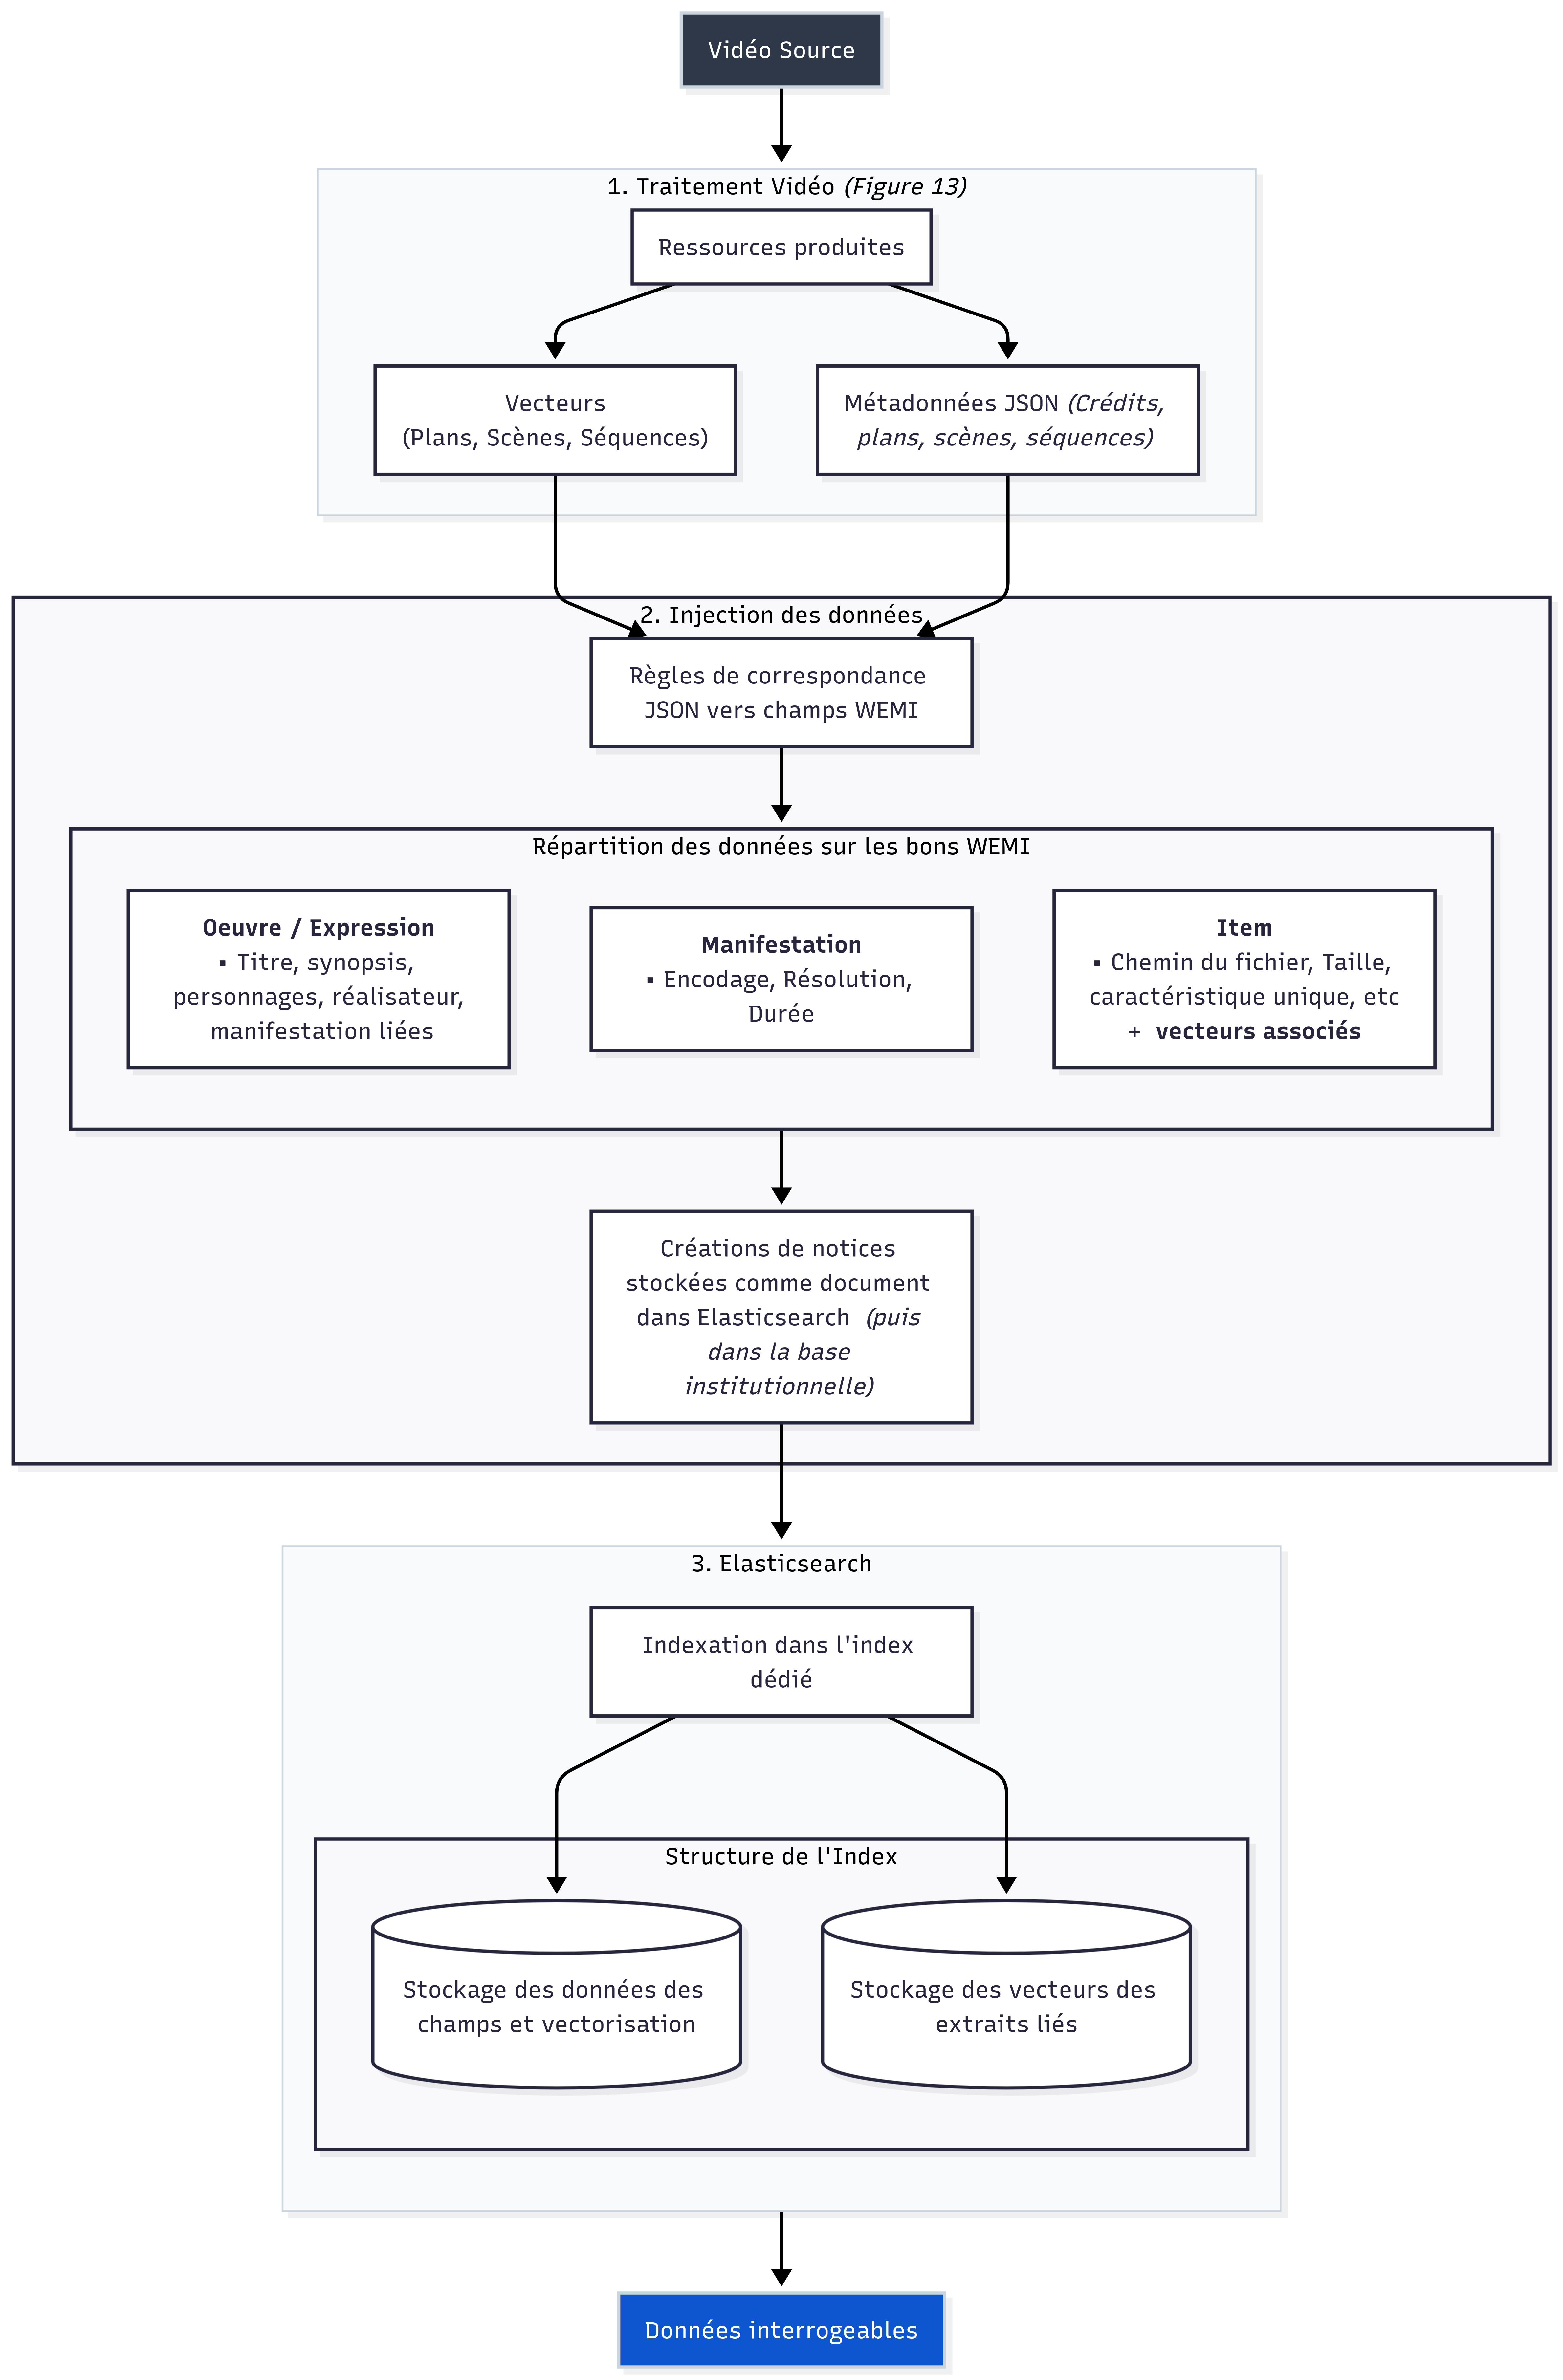
\includegraphics[width=0.8\textwidth]{./Schema/Intégration.png}
	\caption{Schéma du processus d'intégration des données générées par le traitement des \glspl{imgani}.}
	\label{fig:intégration}
\end{figure}

\vspace{0.5cm}

Grâce à la première partie du processus, nous disposons des méta-données à mettre dans les bons champs et niveaux \gls{WEMI} ainsi que des \glspl{vcs} des \glspl{pl}, \glspl{sc} et \glspl{sq} à associé aux notices correspondantes. \newline

Le \coeur de ce processus se situe à notre étape 2. Il s'agit d'assurer l'intégration de ces différentes ressources aux bons endroits applicatifs. Pour les méta-données, il s'agit d'établir des règles de correspondances entre les champs de nos \J et ceux champs de notre index \gls{ES} rattachés aux bons \gls{WEMI}. Grâce à la stabilité du \J et des champs \gls{ES}, on s'assure de la répétabilité de la procédure. 

Pour cela, on établi la structure du \J et la correspondes des champs en amont. Ainsi, on donnera à nos différents outils les \textit{templates} à remplir en fonction de ce qui est attendu. Chaque \textit{template} sera dors et déjà compatible avec les champs \gls{ES} ciblés.

Les \glspl{vcs} étant associé aux \J, ils seront automatiquement rattachés aux bonnes notices \glspl{it}. L'avantage de les stocker dans \gls{ES} est de permettre, par la suite, l'utilisation de la \guillemet{recherche augmentée}. On peut imaginer une utilisation alternative de cette dernière centrée sur la \gls{table} des médias. Une requête basée sur une description d'une action ou d'un thème créer un \gls{vcs} comparable avec ceux des \glspl{pl}, \glspl{sc} et \glspl{sq}. Ce qui permet donc de rechercher des extraits par des requêtes imprécises. 

\subsection{Proposition de conception technique}

Ici, nous allons proposer des outils à utiliser pour ce processus. Notons cependant qu'un tel processus demande des technologie variées. Un effort de réutilisations des mêmes technologies à été menée. Ajoutons que, bien que non estimée, la mobilisation de toutes ces technologies demande des ressources informatiques importantes.\newline

Nous allons prendre chacun de nos deux traitements et présenter les outils à utiliser pour chaque étape en nous concentrant sur leur utilisation dans notre processus.\newline

Commençons par notre processus de traitement\footnote{Voir figure \ref{fig:indexation} page \pageref{fig:indexation}} qui articule au sein d'un script python :

\begin{enumerate}
	
	\item Pour la première étape, nous utilisons PySceneDetect\footnote{Voir \fullref{PyScene}}, FFmpeg\footnote{Voir \fullref{FFmpeg}} et le \gls{VLM} \textit{SmolVLM2-2.2B-Instruct}\footcite{HuggingFaceTBSmolVLM222BInstructHugging2024}. En combinant la détection des ruptures visuelles de PySceneDetect et la manipulation vidéo de FFmpeg, on extrait tous les \glspl{pl}. Avec \textit{SmolVLM2-2.2B-Instruct}, on pourra dès lors lire les crédits et les stocker dans le fichier \J dédié. Nous proposons ce modèle car il est très léger, pesant 2,2 giga octets seulement, tout en étant précis et fiable. 
	
	\item Pour notre seconde étape, l'extraction d'une image clé d'un \gls{pl} et de son extrait audio, FFmpeg l'intègre nativement. C'est une fonction dédiée basée sur la détections des points clés des images et sur la sélection de celles en contenant le plus.
	
	\item Pour notre troisième étape, afin d'identifier et reconnaître les entités, les personnes et l'ambiance sonore nous utilisons 3 outils. SAM2 pour la \gls{seg} et leu suivis des objets\footnote{Voir \fullref{SAM2}}. FaceNet pour la reconnaissance de visages\footnote{Voir \fullref{FaceNet}}. Puis QWEN2-Audio pour l'analyse de la bande son.\footnote{Voir \fullref{QWEN2}}. L'application successive de ces outils, dans un ordre à définir, permet d'identifier les célébrités et d'analyser l'ambiance sonore ainsi que les entités présentes. 
	
	\item Pour notre quatrième étape, celle de \gls{Vecsion} des éléments identifiés, il y a deux approches possibles : 
	
	\subitem L'utilisations de \textit{SmolVLM2-2.2B-Instruct} et QWEN2-Audio pour générer des analyses sémantiques textuelles. Sur ces analyses, nous appliquons notre modèle de \gls{Vecsion} déjà éprouvé \textit{intfloat/multilingual-e5-small}, ou \textit{intfloat/multilingual-e5-base}, pour générer des \gls{vcs}. La problématique se situe dans le fait qu'on génère des \gls{vcs} sur du texte et non à partir de l'image ou du son. Cela implique un intermédiaire pouvant créer un décalage.
	
	\subitem Ou l'utilisation de \gls{mmlts} comme CLIP\footnote{\fullref{clip}} capable d'analyser aussi bien le son que la vidéo. Contrairement aux processus précédent, les \gls{vcs} générés par CLIP à partir des vidéos et sons et non d'analyse textuelles précédemments générées.
	
	\item Pour notre cinquième étape, nous avons recours à une matrice de proximité. C'est une méthode de calcul tabulaire permettant d'établir le degré de similarité entre deux objets à partir de différents éléments. En somme, cela permet d'établir des proximités entre les \glspl{pl} selon leurs \gls{vcs} et leurs horodatages. Ainsi, deux \glspl{pl} à l'horodatage proche seront plus facilement rapproché que deux \glspl{pl} à l'horodatage très éloignés. Cela permet d'éviter de consituer des \glspl{sc} avec des \glspl{pl} éparpillés dans la bande vidéos.
	
	\item Pour la deuxième partie de cette cinquièreme étape, nous utilisons notre \gls{LLM} \textit{Gemma-4-31B}\footnote{Voir \fullref{Gemma}} afin d'analyser tous les \J des \glspl{pl} rassemblé et de constituer un \J pour la \gls{sc}.
	
	\item Pour les séquences et \gls{oe}, aux étapes 6, 6 \guillemet{bis} et 7, nous réitérons ce traitement. En effet, le traitement n'est guère différent si ce n'est qu'on ne l'applique plus aux \glspl{pl} mais aux \glspl{sc}. Cela ne nécessite pas de changement. 
\end{enumerate}

Pour le processus d'intégration des données dans l'application, les technologies sont déjà présente. En effet, pour notre étape numéro 3 sur le stockage et la mise à disposition des données dans \gls{ES}, c'est le logiciel qui s'en charge. Nous n'avons donc pas d'ajout à effectuer.

Cependant, l'étape précédente d'injection des données demande une technologie précise afin de créer les correspondances de champs entre les \J et \gls{ES}. La librairie \textit{Pydantic}, déjà utilisée pour la \textit{recherche augmentée}, permet d'établir et de vérifier ces règles en amont. L'intégration est alors exécuté après validation des fichiers \J. Les \gls{vcs} sont quant à eux déjà pris en charge par un module spécifique d'\gls{ES}.\newline

Ce processus mobilise un grand nombre de technologies différentes, certains sont assez volumineuse même lorsqu'on prend les options \guillemet{légères}. Nous pensons notamment aux \gls{VLM} et \gls{ALM} qui mobilisent énormément de ressources.  

Le poids du processus est donc conséquent. Il s'agit de procéder à énormément de calcul complexes dans une chaîne de traitement iétrative. En effet, elle s'applique sur chaque image clés de chaque \gls{pl} sachant qu'une \gls{oe} cinématographique peut se composer aisément de plus de 1000 images clés. C'est donc un processus long, répétitf et très demandeurs en ressources. Modifier le processsus pour traiter toutes les images clés en lots, et non successivement, ne représente pas une solution. Cela risque de saturer la \gls{RAM} et les capacités des outils conduisant à des hallucinations. 

\subsection{Proposition de conception du parcours utilisateurs}

Nous allons ici procéder à une analyse afin d'identifier les points d'attentions en terme d'\gls{ux} et d'\gls{ui}.\newline

D'abord, le processus présenté est pensé comme étant interne à l'application. Ce qui demande donc de le connecter à des éléments déjà présents afin de ne pas perturber l'utilisateur. C'est ce que nous avons fait avec la \guillemet{recherche augmentée}. Dans SkinSoft l'utilisateur à la possibilité d'intégrer des fichiers dans le logiciel par simple \guillemet{glisser / déposer}. On peut alors penser qu'au moment de déposer une vidéo, l'application genère une fenêtre d'interraction demandant à l'utilisateur de choisir soit une intégration simple, soit l'indexation semi-automatisée.

Il faut établir un choix et message clair, permettant de faire comprendre qu'il ne s'agit de produire automatiquement une indexation mais d'en suggérer une. À ce titre, l'humain garde son rôle de décisionnaire et peu valider, modifier ou invalider la production. Si l'utilisateur choisi l'indexation semi-automatiséen alors le processus décrit s'applique. Cependant, ce processus doit s'appliquer sous contrôle de l'utilisateur. Ce qui demande donc une interface et une expérience d'utilisations.\newline

Cela nous amène à la notion de choix. Notre processus est complexe et prend en charge divers aspects de traitement. La division d'une vidéo à différentes échelles, l'extractions de différentes données et la création de notices \gls{WEMI} pré-remplies. Chacun de ces aspects demande des choix utilisateurs. 

En premier lieu, il se peut qu'un utilisateur ne souhaite pas diviser sa vidéo en unité plus petites notamment car il s'agit déjà d'un extrait. Il faut donc offrir cette possibilité

Ensuite, il se peu que l'utilisateur souhaite créer l'\gls{it} d'un \gls{WEMI} préexistant. Au quel cas, l'analyse des crédits et l'analyse d'éléments appartenants aux niveaux \gls{oe} et \gls{exp} ou \gls{man} ne sont pas nécessaire. 

Enfin, il se peut également qu'un utilisateur souhaite seule compléter des notices préexistantes. Cet usage implique un changement de la fonctionnalité afin qu'elle s'applique sur des éléments préexistants, et des champs déjà remplis.\newline

Chacun de ces cas d'usages place la notion de choix au \coeur de l'\gls{ux} et de l'\gls{ui}. Cela implique que la fonctionnalité doit être hautement modulable afin de répondre à différentes attentes simples comme complexes. Ainsi l'\gls{ux} doit être basée sur la notion de choix et l'\gls{ui} doit présenter une interface permettant à l'utilisateur de moduler la fonction. Cela peut se faire via la sélection ou déselection de certaines options de traitements. \newline

De plus, il faut offire la possibilité de modifier, valider ou invalider le travail effectué à chaque étape de traitement. Par exemple, le découpage en \glspl{pl}, \glspl{sc} ou \glspl{sq} peut ne pas être satisifaisant, ainsi une interface doit permettre de modifier cela simplement. Cela doit aussi être valable pour les données générées dans les \J. Il faut penser à une façon de présenter les informations en retirant l'aspect technique du \J. Cela peut être par une pré-visualisation de la notice créée avec les champs pré-remplis avec les données correspondantes. Les modifications effectuées ici se répliquent ensuite sur le fichier \J.\newline

En somme, l'intégration des questions du parcours utilisateurs, centré sur une approche \textit{human in the loop}, complexifie techniquement le processus. Notamment en imposant divers stade de gestion d'erreur et une modularité du code. 

De plus, le nombre d'éléments à prévoir en terme de validation et d'étape de contrôle demande une interface dédiée. Ce qui amène à complexifier encore le \gls{sgc} par l'ajout d'une fonctionnalité supplémentaire avec sa propre expérience et interface. 

\subsection{Apports et limites}

Le processus que nous avons dépeint met en lumière plusieurs éléments quant à la possibilité de s'appuyer sur des processus semi-automatisé pour traiter de telle typologie. Mais il est important de mettre en lumière l'apport de ces outils, mais aussi leurs limites. L'indexation semi-automatisée est une solution très contrastée, renouvelant des problématique et en créant de nouvelles. 

Ce processus, qui n'a pas encore fait l'objet d'un \textit{proof of concept}, semble ouvrir la voix au traitement automatisée de cette typologie documentaire. Différents outils sont aujourd'hui articulable afin de répondre aux besoins les plus précis de traitement de cette typologie documentaire. Mais ce processus tout à fait conceptuel présente des difficultées majeures. \newline

Ce processus présente deux avantages majeurs. Le premier est la possibilité de traiter des \gls{oe} d'\gls{imgani} de plusieurs heures à la chaîne, et sans interventions humaine. Cela permet de décharger l'utilisateur de l'analyse manuelle de plusieurs heures de bande vidéos, et lui permet de s'occuper d'autres tâches. Le second avantage c'est ça répétabilité. Par la production de \J dans un format fixe et interfacée avec les index \gls{ES} concernés, ce processus est très stable. On s'assure d'extraire les mêmes métadonnées et de les intégrer toujours au même endroit. 

Il faut ajouter à cela qu'il reste simple d'usage. Il suffit d'entrer une \gls{oe}, de laisser le traitement s'accomplir, puis de contrôler à chaque étape afin de rectifier. Le seul défaut, est que la plus part des outils ne peuvent pas faire l'objet d'un \gls{ft}. Prenons l'exemple de PySceneDetect, il s'appuis sur la \gls{CV} algorithmique c'est à dire sans \gls{IA}. Si les détections de changements de plans sont erronnés, la correction manuel par l'utilisateur n'entraîne pas d'améliorations à long terme.

Nous pouvons également dire qu'il reste largement flexible. Par exemple, le modèle SAM2 est parfaitement compatible avec un \gls{mod} YOLO\footnote{Voir \url{https://www.ultralytics.com/fr/yolo} pour plus d'informations} pour la détection et l'identification d'objets précis. Ou bien encore le \gls{mod} FaceNet peut s'entraîner sur une base de données constituée par l'institution pour détecter des personnalités précises. De cette manière, le processus est très souple et offre diverse possibilité d'adaptation intéressante.\newline

Les limites sont également nombreuses. D'abord l'absence de reconnaissance de la typologie de l'\gls{imgani}. En effet, dans ce processus nous n'avons pas incorporer ce principe de détection typologie car nous ignorons l'efficacité de ces technologies à accomplir cette tâche. 

En effet, les \gls{VLM} et \gls{mmlts} sont entraînés pour déterminer et décrire ce qu'il se passe au sein d'une image ou d'une \gls{sc}. Ils peuvent aller plus loin par des analyses colorimétriques, et sonore avec des \gls{ALM}, afin de déterminer le ton du film, le sentiment qui s'en dégage. Cependant, nous n'avons rien trouver au sujet de leurs capacité à distinguer un film muet, d'un film en couleur et sonore, d'un film d'animation. 

Sans que cela semble impossible, aujourd'hui les outils que nous possédons sont trop peu entraînés et spécialisé sur ce domaine. D'autant que la typologie d'un objet patrimonial peut ne pas correspondre à une typologie publique. Ajoutons également que certaines typologie se distingue par des nuances très fines. Par exemple comment distinguer une \gls{imgani} professionnelle d'une \gls{imgani} amateur ? Elle se distingue par les moyens de productions, la possibilité de reconnaître les personnes qui s'y trouvent et la présence d'une construction sémantique de l'\gls{oe}. Mais toutte ces dimensions semblent difficile à être prise en compte.

Ajoutons à cela le fiabilité des métadonnées générées. Concernant la fiabilité, nous en revenons à notre problématique d'hallucination des \gls{mod} d'\glspl{IA} sur lequel nous n'avons que peu de contrôle. Étant au \coeur des données patrimoniales, puisqu'il s'agit de la produire, le contrôle de ce phénomène est important. \newline

\newpage

\chapter{Impact potentiel des outils sur les données et collections patrimoniales}

% !TeX root = ../document_maitre.tex

Ces innovations technologiques promettent des évolutions importantes pour les \glspl{sgc} et le monde professionnel concerné. Elles ont pour but d'accompagner les professionnels face aux nouveaux défis et enjeux de la gestion des collections. Pour cela, on a identifié trois axes d'améliorations :

L'axe de l'accessibilité aux données stockées, par une recherche plus intuitive et puissante qu'est la \guillemet{recherche augmentée}. Celui de l'accessibilité applicative et d'appuis à la production, pour une meilleure maîtrise de son environnement de travail, ce qu'aborde notre \gls{chatbot}. Et enfin celui de la production massive des données patrimoniales par un processus d'indexation semi-automatisée des \glspl{imgani}.\newline

Ces outils sont pensés pour \guillemet{révolutionner} ces trois axes par l'apport de solution simple, immédiate et fiable. Nous avons démontré que cela n'est pas réellement possible, ces outils étant faillibles et hautement évolutifs.  

Mais il faut surtout comprendre que de tels outils ne \guillemet{révolutionnent} par la gestion des collections patrimoniales mais impactent profondément diverses couches de cet univers métier. L'impact de ces outils n'est pas seulement technique, il est aussi juridique et éthique venant jusqu'à questionner et redéfinir des acquis.

Ainsi, pour chaque outil, nous allons aborder de front les questions soulevées par leurs implémentations dans les \gls{sgc}, au \coeur des pratiques et données des collections patrimoniales.

\subsection{La recherche augmentée}

Cet outil à une position intéressante car il s'agit, finalement, de transposer les pratiques de recherche grand public sur internet dans le logiciel. Ce qui dès lors crée des porosités entre notre position d'utilisateur d'internet, et celle d'utilisateur de logiciel métier. Nos pratiques publiques influent sur notre conception de concept que l'on retrouve dans le domaine professionnel, ce qui amène à un effort de création de lien entre les deux mondes afin d'unifier les pratiques.

Finalement cet outil amène à mélanger aux pratiques professionnelles des attentes \guillemet{grand public}. Aujourd'hui, lorsque l'on utilise un moteur de recherche, on formule instinctivement une phrase. Avec les \gls{ac}, c'est une dimension encore plus forte, qui entre de plus en plus dans nos habitudes. Ainsi, un mode de recherche traditionnel par mots-clés provoque un sentiment de frustration même au sein d'un logiciel métier. 

Cela pose donc un questionnement éthique important sur cette porosité entre l'usage public et l'usage professionnel. À quel moment l'infusion d'attentes et de pratiques \guillemet{grand public} dans des logiciels métier doit-elle s'arrêter ? On peut peux penser au moment où de telles pratiques mettent en danger les valeurs fondamentales de l'univers professionnel.\newline

Juridiquement, cela pose les entreprises fournisseuses de \gls{sgc}, comme SkinSoft, dans une position délicate. Elle propose un outil d'\gls{IA} traitant, sur son propre serveur, des données patrimoniales d'une institution tierce. Juridiquement, cela pose l'entreprise comme responsable de la conservation des données et de leur sécurité. Cela demande un contrôle total du traitement exécuté sur les données par le processus. 

Cette double responsabilité est encadrée par le \gls{RGPD}.\footnote{Voir \fullref{juridique}} Mais le développement de tels outils et leur popularité croissante dans ce contexte, peut amener à questionner sa pertinence. Ou plutôt son application à de tels processus demandant des redéfinitions juridiques pour un meilleur encadrement dans ce domaine. 

\subsection{Le \gls{chatbot}}

Pour le \gls{chatbot}, nous pouvons retrouver les mêmes considérations juridiques dès lors que nous le pensons comme assistant de contrôle de la qualité des données. Son accès aux données patrimoniales et sa capacité à les traiter posent les mêmes questions juridiques. 

Mais ce n'est pas l'aspect le plus important de cet outil. Les implications et enjeux sont bien plus d'ordre éthique et des pratiques métiers, que de l'ordre juridique.

Le premier élément est la redéfinition du rapport de l'utilisateur avec ses propres données. En effet, disposer d'un moyen de contrôle rapide, accessible et efficace peut-il impacter la productivité ? La possession d'un moyen de contrôle alimenté par de l'\gls{IA} peut pousser à croire à une infaillibilité de ce dernier et donc à baisser sa vigilance. Sans être une conséquence inévitable, c'est une considération éthique qu'il convient d'observer. 

Cela questionne directement le type d'outils que l'on doit et peut offrir dans un \gls{sgc}. Comment les concevoir afin de constituer un outil d'appui sans remplacer l'utilisateur humain ou créer un relâchement de sa vigilance ? Où se situe la frontière entre l'outil d'appui, et l'outil de remplacement ? 

Le \gls{chatbot} entre directement dans ces questions. Automatiser des tâches de contrôle et d'assistance par \gls{IA} ne risque-t-il pas de modifier trop profondément le rapport de l'utilisateur à son logiciel métier ? Trop de simplicité apportée par des outils provenant du quotidien peut-elle représenter un danger pour la productivité et la posture professionnelle des utilisateurs ? 

Nous ne saurons apporter de réponses. Cependant, il est certain que des réflexions éthiques et méthodologiques seront à mener vis-à-vis de ces outils. Il faut peut-être envisager d'encadrer les pratiques utilisateurs, en commençant par limiter l'impact de ces outils sur un équilibre professionnel préexistant.

\subsection{L'indexation semi-automatisée des \glspl{imgani}}

Mise à part des enjeux techniques et des questions d'\gls{ux} et d'\gls{ui}, cet outil remet en question des principes fondamentaux.\newline

D'abord le principe de rigueur scientifique. Contrairement à la \guillemet{recherche augmentée} ou au \gls{chatbot}, ici on génère de la donnée à valeur scientifique. Ce processus s’appuie sur des formes d'\gls{IAG} : les \gls{LLM}, \gls{VLM} et \gls{ALM}. La génération des données par ces outils peut être compromise par des hallucinations impactant la qualité des données et donc la rigueur scientifique.

Nous en revenons à la même problématique rencontrée avec la \guillemet{recherche augmentée}. La particularité ici est qu'une architecture \gls{RAG} n'est pas applicable. Cela contraint à adopter des architectures \textit{human in the loop} assez lourdes, pouvant compromettre le gain de temps que l'on cherche à obtenir. Il faut donc penser et établir de nouveaux procédés de contrôle des hallucinations afin de certifier une rigueur scientifique suffisante.

Ensuite, le principe de confiance. Fragiliser la véracité des informations des bases de données institutionnelles amène à provoquer des doutes dans l'usage de ces applications et dans les données produites. Ce qui, à plus large échelle, peut conduire à une méfiance du public auquel on diffuse ces informations.

On entre ici dans un domaine flou, à la croisée entre le procédé technique et les questions d'\gls{ux} et d'\gls{ui}. Habituellement, ces deux domaines permettent de rassurer l'utilisateur dans son usage d'une fonctionnalité. Mais devant la complexité de ces processus et les risques d'hallucinations, cela ne semble plus être suffisant. Il y a donc une demande de nouveaux moyens.\newline

Il se pose également la question de la provenance des données indexées. Les institutions conservatrices ont l'obligation de retracer la provenance des données conservées. On entre dans une limite juridique et éthique au sujet de l'\gls{IA}. Doit-on préciser que cela à été extrait par \gls{IA} ? Ou doit-on pousser l'\gls{IA} à citer les sources ? Le cadre juridique impose de préciser quand un contenu est généré par \gls{IA}\footnote{Voir \fullref{juridique}}. Mais lorsqu'il s'agit d'une donnée produite dans de tels processus, où l'\gls{IA} ne sert que d'extracteur, devons-nous le préciser ?  

Ainsi, il y a une redéfinition profonde des pratiques métiers dans la conservation du patrimoine. L'utilisateur du \gls{sgc} n'est plus créateur de la donnée, mais vérificateur et validateur ce qui change le paradigme.\newline

\subsection{Conclusion}

Finalement, l'implémentation de tels outils possède trois niveaux de complexités. Technologiques d'abord, car les problématiques, défis et attentes sont hétérogènes et complexes. De l'ordre éthique ensuite car leur implémentation et usage bouleversent des pratiques et valeurs portées par le monde de la gestion des collections. L’adaptation à ces éléments et nécessaire, mais il existe un fossé important pouvant demander une adaptation inversée. Et enfin juridique car ces outils peuvent être assez opaques et représenter des menaces face au principe de gouvernance des données. 

Nous sommes aujourd'hui au début de ces transformations profondes. Les outils ne sont pas encore mûr, et leurs utilisations professionnelles dans la gestion des collections pas encore effective. Cependant, elles annoncent d'ores et déjà des transformations importantes de cet univers professionnelles qu'il nous faut maîtriser et diriger.

	%etc.
	
	
\part*{Conclusion}
	% !TeX root = ../document_maitre.tex

Patrimoine et gestion des collections sont des domaines étroitement liés, actuellement en proie à des difficultés exarcerbée et, pense-t-on, à l'aube d'une révolution technologique. 

La double hétérogénéité des collections, des données informatiques générées ainsi que leurs masses sont aujourd'hui des problématiques fondamentales. Chaque typologie patrimoniale connaît ses propres normes et standards de descriptions, ainsi que ces propres modèles conceptuel de gestions. Leurs numérisation dupplique les obligations et besoins de gestion, comme nous l'avons vus avec l'\gls{imgani} où cette double nature amène de doubles enjeux de conservations. Et enfin, leurs masses, dûs au phénomène de \gls{bgdt}, complexifie les efforts d'harmonisation et de gestions. 

Les \gls{sgc} sont au \coeur de nos pratiques de gestion des collections. Plus que de simple registre numérique, ce sont de véritables outils stratégiques afin de piloter la vie des collections et institutions conservatrices. L'évolution des difficultés et des besoins dans ce domaine ont toujours amenée ces logiciels à s'adapter. L'intégration des normes et standards, l'applications de l'\gls{intero} et des modèles conceptuels sont aujourd'hui prise en compte, comme nous l'avons vus avec la suite SkinSoft.

Mais aujourd'hui, la \gls{bgdt} amène un renouveau des difficultés et ne ces dernier ne semblent plus disposer des moyens de s'y adapter pleinement. Le problème majeur se situe en amont du logiciel : lors de la production et de l'intégration des données. Par exemple, pour l'\gls{imgani} les \gls{sgc} ne proposent pas de solution concrète de facilitation d'une indexation fastidieuse. Situé au \coeur de ces derniers, l'indexation humaine de telles typologies patrimoniales est ajourd'hui limitée. Elle ne permet plus de traiter à un rythme suffisant la masse de données entrante. Ajoutons que les modalités de gestion très spécifiques et maléables de ces typologies rendent leurs intégrations de manière simple et ergonomique assez complexe à établir. 

Ces logiciels ont alors deux limites principales face aux évolutions des pratiques aux enjeux du \gls{bgdt} dans notre milieu. D'abord fonctionnelle, car ils n'arrivent plus à faciliter les processus d'indexation et de gestion des données entrantes dans des modèles de gestion complexes. Ensuite ergonomiques, car la nature complexe de ces logiciels n'offre plus de moyen de repères suffisant afin d'aborder sereinement cet outils de travail.\newline

Aujourd'hui, l'\gls{IA} est en plein essort et se fait remarquer par sa capacité de traitement en autonomie de très grandes volumétries de données. Mais également pour sa capacité d'interraction avec d'autres logiciels. 

Dans le domaine patrimonial, nous solicitons surtout les technologies de \gls{NLP}, \gls{RAG} et de \gls{CV}. L'utilisation de ces outils est paradoxale : rapidement utilisé de différentes manière pour le patrimoine, la recherche semble aujourd'hui préférer une utilisation pour l'accessibilité grand public. Leurs applications à la sphère professionnelles pour la production de métadonnées s'oppose à des principes de rigueur scientifique. En effet, leurs capacités à halluciner constitue un risque de corruption du bien fondé des bases de données institutionnelles. Vraisemblablement, cela amène à repousser le moment d'intégration de ces outils.

Cependant, ces technologies propose des pistes prometteuses pour soulager, si ce n'est résoudre, la plus parts des difficultés actuelles des \glspl{sgc}. Le \gls{RAG} et le \gls{NLP} sont prometteur afin de permettre des recherches plus naturelles, fines et faciles dans sa propre base de données. La capacité de ce dernier à \guillemet{comprendre} le langage humain semble en faire un parfait intermédiare entre l'application et l'humain. Pour la \gls{CV}, c'est sa capacité à analyser des images, identifier et exploiter des caractéristiques clés dans des résumés sémantiques qui représente une voie d'amélioration de l'indexation de l'\gls{imgani}. 

Ces outils peuvent répondre aux difficultés fonctionnelles, par des processus d'indexation automatisée en interaction avec des \gls{thesaurus} par exemple. Mais aussi aux difficultés ergonomiques en facilitant l'accessibilité à l'outil et aux données, peut être même jusqu'à appuyer l'homogénéisation des données. De tels outils semblent être prometteurs pour appuyer les professionnels dans leurs diverses tâches de production et d'utilisation des \glspl{sgc}. \newline

Ces outils n'ont pas encore été pensés pour une intégration au \coeur de \gls{sgc}. Cela pose donc la question de la faisabilité technique et de l'impact potentiel sur les pratiques et fonctionnement de ces logiciels. 

Nous avons donc suivi cette piste en se demandant comment intégrer de tels technologies dans le logiciel SkinSoft, dans quel but et surtout quels en sont les enjeux. Cela à aboutit à explorer les deux axes à l'aide d'outils pensé pour appuyer les professionnels. D'abord l'axe ergonomique avec la \guillemet{recherche augmentée} pour une amélioration de la pertinence des résultats et une facilité d'interrogation des données institutionnelles. Mais également avec le \gls{chatbot}, pensé pour accompagner l'utilisateur dans son utilisation de l'application et ses missions de contrôle de la qualité des métadonnées indexées. Mais également l'axe fonctionnel avec l'indexation semi-automatisées des \glspl{imgani}, représentant un volume très importants de données à intégrer selon des exigences normatives variables et exigeante. 

Nos différentes explorations, encore très conceptuelles, de ces outils nous amène à différents constats. D'abord, l'inégalité des contraintes techniques et des faisabilités technologiques. Des processus comme la \guillemet{recherche augmentée} sont aujourd'hui basés sur des technologies plus stables et moins gourmandes en ressources qu'un processus d'indexation semi-automatisée de l'\gls{imgani}. Ce dernier semblant dès lors bien plus inaccessibles que la \guillemet{recherche augmentée}, à cause de sa complexité et de sa demande en ressources complexe à satisfaire. 

Nous démontrons que la réussite de ces outils ne dépendent pas de ces seuls question. Ce sont en effet des conditions préalables à la réalisations de ces outils, mais l'enjeu final de l'adoption de l'outil réside dans d'autre domaine. À savoir l'\gls{ux} et l'\gls{ui}, en charge de la facilité d'utilisation de ces outils. De cette facilité d'usage dépend l'adoption de ces outils par les professionnels du patrimoine. C'est finalement ce degré d'adoption de l'outil qui transforme ou non nos pratiques. Ce qui finalement place les questions d'\gls{ux} et d'\gls{ui} au \coeur des enjeux. 

De plus, de tels outils s'inscrivent dans un cadre réglementaire et technique strict. Le patrimoine et la gestion des données sont riches en contraintes et exigence. La souveraineté des informations, la protection du droit d'auteur, et la conformité au cadre juridique de l'\textit{AI Act} sont des enjeux capitaux. Plus que la performance, un bon outil d'appui aux professionnels dans un \gls{sgc} est avant tout un outil respecteux et conforme à cet univers.

Sur le plan éthique, l'intégration de tels outils est aussi problématique. Ils questionnent des valeurs d'honnêteté, de rigueur et d'exhaustivité scientifique dans les bases de données institutionnelles. Combinés aux facteurs juridiques, cela réaffirme que l'automatisation ne peut être totale. L'approche de ces outils doit être évolutive et prudente. Cela passe par des architectures \textit{(human-in-the-loop)}, demeurant la condition \textit{sine qua non} d'une exploitation éthique, pérenne et acceptée.\newline

Finalement, l'implémentation d'outils d'\gls{IA} peu permettre de répondre aux défis actuels de deux manières. D'abord par l'augmentation de l'accessibilité et de la facilité d'usage des \gls{sgc} et des bases de données patrimoniales. Bien qu'assez largement ignorés aujourd'hui, nous avons démontré que la première limite de ces logiciels viens de leurs propres architecture logicielle. Les \glspl{chatbot} et recherche assistées par \gls{IA} peuvent permettre d'en améliorer l'accessibilité, d'en facilité l'usage et d'offrir des expériences d'utilisations plus confortables créant de meilleur conditions de productions. 

Ensuite par l'automatisation relative de chaîne d'indexation sur certaines typologies documentaires. Bien que notre essais sur l'\gls{imgani} ai montré toute la complexité et les limites d'un tel processus, on peut penser qu'appliqué à des objets plus structuré et traités comme des archives, de tels processus puisse être réalisable. Cependant, la consommation de ressources de ces outils et les danger de l'hallucination demandent à en relativiser l'application. \newline

Cette étude nous permet finalement de répondre à notre problématique initiale. Ces technologies peuvent améliorer nos utilisations des \glspl{sgc} et nos capacités d'indexations, sans pour autant les révolutionner étant donné leurs limites. Ainsi, ils ne peuvent remplacer l'expertise humaine. L'arrivée de ces outils dans tels domaines de production amènent des réflexions éthiques et juridique qui convergent vers leurs rationnalisation pour en faire des outils d'appuis, de facilitation et non de remplacement. 

Loin de \guillemet{dénaturer} nos pratiques, il est naturel que ces dernières évoluent sans pour autant changer drastiquement. Et il est aujourd'hui de notre responsabilité d'ériger ces cadres éthiques, juridiques et technologiques pour une conception et une utilisation raisonnée de tels outils, cruciaux pour répondre aux défis de la gestion des collections.

	\addcontentsline{toc}{chapter}{Conclusion}
	

	
\newpage{\pagestyle{empty}\cleardoublepage}
	






%%%%%%%%%%%%%%%%%%

\appendix %Des appendices: tables figures, etc

\chapter[Github des livrables techniques]{Github des livrables techniques}

% !TeX root = ../document_maitre.tex

\textbf{Lien :} \url{https://github.com/floflo-boop/Livrable-technique}\newline

Ce dépôt \textit{Github} se constitue de deux documents PDF. Ce sont des documents produits dans le cadre du stage à propos de la création de la fonctionnalité de \guillemet{recherche augmentée}.\footnote{Ces documents professionnels sont la propriété de l'entreprise et ne peuvent être diffusés librement} L'objectif de ce dépôt est de montrer ce qui a été mis en place pour la fonctionnalité de \guillemet{recherche avancée} bien que cela ne soit pas exhaustif.\newline

Le premier document \textit{spécification.pdf} contient la spécification rédigée afin d'établir la fonctionnalité de la \guillemet{recherche augmentée}. Elle explicite les attendus et permet d'établir les règles et fonctions à mettre en place pour l'expérience et l'interface utilisateur.

Loin d'être un document \guillemet{technique} au sens qu'il ne développe pas de processus, ni de code, son objectif est de contraindre le développement de la fonctionnalité par un raisonnement centré sur l'adoption de l'outil par l'utilisateur. C'est donc un document de contrainte afin de réaliser les attentes utilisateurs dans une fonctionnalité, et non l'inverse.\newline

Le second document \textit{index.pdf} est un index \gls{ES} commenté pour être utilisé par la fonctionnalité de \guillemet{recherche augmentée}. L'objectif est de montrer comment ce structure un index \gls{ES} et comment les exploiter pour cette fonctionnalité. Il faut garder en tête que chaque index doit être commenté de cette manière afin de faire fonctionner la \guillemet{recherche augmentée}.

\newpage{\pagestyle{empty}\cleardoublepage}

%%%%%%%%%%%%%%%%%%

\backmatter % glossaire, index, table des figures, table des matières.. (la bibliographie a déjà été appelée)

\printindex
\printglossaries
%\listoftables
\listoffigures
\tableofcontents
\end{document}
